\ifcsname ispublic\endcsname
    \documentclass[11pt,a4paper,notitlepage,fleqn,final]{article}
\else
    \documentclass[11pt,a4paper,notitlepage,fleqn,final]{article}
\fi

\usepackage{amsmath}
\usepackage{amsfonts}
\usepackage{amssymb}
\usepackage{libs/commath2}
\usepackage[table]{xcolor}
\usepackage[hidelinks]{hyperref}
\usepackage[skins,theorems]{tcolorbox}
\usepackage{titlesec}
\usepackage{circuitikz}
\usepackage{pgfplots}
\usepackage{mathtools}
\usepackage[makeroom]{cancel}
\usepackage{mathrsfs}
\usepackage{wrapfig}
\usepackage{subcaption}
\usepackage{floatrow}
\usepackage{esint}
\usepackage{enumitem}
\usepackage{bm}
\usepackage{relsize}
\usepackage{xfrac}
\usepackage{comment}
\usepackage{siunitx}
\usepackage{MnSymbol}
\usepackage[obeyDraft]{todonotes}
\usepackage[linesnumbered,lined]{algorithm2e}


\pgfplotsset{compat=1.13}
\usetikzlibrary{arrows.meta}
\usetikzlibrary{patterns}
\usetikzlibrary{decorations.pathmorphing,patterns}
\usetikzlibrary{decorations.markings}
\usetikzlibrary{backgrounds}
\usetikzlibrary{shapes.misc}
\usetikzlibrary{shapes.multipart}
\usetikzlibrary{shadows.blur}
\usetikzlibrary{snakes}
\usetikzlibrary{fadings}
\usetikzlibrary{intersections}
\usetikzlibrary{arrows.meta}
\usetikzlibrary{calc}
\usetikzlibrary{matrix}

\tcbuselibrary{breakable}

\tikzset{cross/.style={cross out, draw,
        minimum size=2*(#1-\pgflinewidth),
        inner sep=0pt, outer sep=0pt}}
\tikzset{
    mark position/.style args={#1(#2)}{
        postaction={
            decorate,
            decoration={
            	post length=1mm, % ??? Magic to fix "Dimension
            	pre length=1mm, % ???  too large" errors.
                markings,
                mark=at position #1 with \coordinate (#2);
            }
        }
    }
}

\pgfmathdeclarefunction{sinc}{1}{%
	\pgfmathparse{abs(#1)<0.01 ? int(1) : int(0)}%
	\ifnum\pgfmathresult>0 \pgfmathparse{1}\else\pgfmathparse{sin(#1 r)/#1}\fi%
}
\pgfmathdeclarefunction{gauss}{2}{%
	\pgfmathparse{1/(#2*sqrt(2*pi))*exp(-((x-#1)^2)/(2*#2^2))}%
}

\usepackage[left=2cm,right=2cm,top=2cm,bottom=2cm]{geometry}

%\usepackage[no-math]{fontspec}
\usepackage{fontspec}
%\usepackage{mathspec}
\usepackage{unicode-math}
\setmainfont{texgyretermes-regular.otf}
\setsansfont{texgyreheros-regular.otf}
%\newfontfamily\greekfont[Script=Greek]{Linux Libertine O}
%\newfontfamily\greekfontsf[Script=Greek]{Linux Libertine O}
\usepackage{polyglossia}
\newfontfamily\greekfont[Script=Greek]{texgyretermes-regular.otf}
\newfontfamily\greekfontsf[Script=Greek]{texgyreheros-regular.otf}
\newfontfamily\greekfonttt[Script=Greek]{Latin Modern Mono}
%\usepackage[greek]{babel}
\setdefaultlanguage{greek}
\setotherlanguage{english}
\newcommand{\textlatin}[1]{#1}
%\newcommand{\mathlarger}{}

%\usepackage[utf8]{inputenc}
%\usepackage[greek]{babel}


%\usepackage{tkz-euclide} % loads  TikZ and tkz-base
%\usetkzobj{angles} % important you want to use angles

\newlist{enumparen}{enumerate}{1}
\setlist[enumparen]{label=(\arabic*)}
\newlist{enumpar}{enumerate}{1}
\setlist[enumpar]{label=\arabic*)}

\newlist{enumgreek}{enumerate}{1}
\setlist[enumgreek]{label=\alph*.}
\newlist{enumgreekparen}{enumerate}{1}
\setlist[enumgreekparen]{label=(\alph*)}
\newlist{enumgreekpar}{enumerate}{1}
\setlist[enumgreekpar]{label=\alph*)}


\newlist{enumroman}{enumerate}{1}
\setlist[enumroman]{label=(\roman*)}

\newlist{enumlatin}{enumerate}{1}
\setlist[enumlatin]{label=(\alph*)}

\newlist{invitemize}{itemize}{1}
\setlist[invitemize]{noitemsep,label=}

\usepackage{letltxmacro}

\LetLtxMacro\OriginalLongrightarrow\Longrightarrow
\LetLtxMacro\OriginalLongleftarrow\Longleftarrow

% Implement new macros
% --------------------
\usepackage{trimclip}
\DeclareRobustCommand\Longrightarrow{\NewRelbar\joinrel\Rightarrow}
\DeclareRobustCommand\Longleftarrow{\Leftarrow\joinrel\NewRelbar}

\makeatletter
\DeclareRobustCommand\NewRelbar{%
  \mathrel{%
    \mathpalette\@NewRelbar{}%
  }%
}
\newcommand*\@NewRelbar[2]{%
  % #1: math style
  % #2: unused
  \sbox0{$#1=$}%
  \sbox2{$#1\Rightarrow\m@th$}%
  \sbox4{$#1\Leftarrow\m@th$}%
  \clipbox{0pt 0pt \dimexpr(\wd2-.6\wd0) 0pt}{\copy2}%
  \kern-.2\wd0 %
  \clipbox{\dimexpr(\wd4-.6\wd0) 0pt 0pt 0pt}{\copy4}%
}
\makeatother


\makeatletter
\pgfdeclareradialshading[tikz@ball]{ball}{\pgfqpoint{0bp}{0bp}}{%
	color(0bp)=(tikz@ball!50!white);
	color(10bp)=(tikz@ball!50!white);
	color(15bp)=(tikz@ball!70!black);
	color(20bp)=(black!70);
	color(30bp)=(black!70)}%
\makeatother


\makeatletter
\let\anw@true\anw@false

%\newcommand{\attnboxed}[1]{\textcolor{red}{\fbox{\normalcolor\m@th$\displaystyle#1$}}}
\makeatother
\tcbset{highlight math style={enhanced,colframe=red,colback=white,%
        arc=0pt,boxrule=1pt,shrink tight,boxsep=1.5mm,extrude by=0.5mm}}
\newcommand{\attnboxed}[1]{\tcbhighmath[colback=red!5!white,drop fuzzy shadow,arc=0mm]{#1}}
\titleformat{\section}{\bf\Large}{Κεφάλαιο \thesection}{1em}{}
\newtcolorbox{attnbox}[1]{colback=red!5!white,%
    colframe=red!75!black,fonttitle=\bfseries,title=#1}
\newtcbox{quickattnbox}[1]{colback=red!5!white,%
	colframe=red!75!black,fonttitle=\bfseries,title=#1}
\newtcolorbox{infobox}[1]{colback=blue!5!white,%
    colframe=blue!75!black,fonttitle=\bfseries,title=#1}

\AtBeginDocument{%
\let\arg\relax
\let\Re\relax
\let\Im\relax
\DeclareMathOperator{\arg}{Arg}
\DeclareMathOperator{\Re}{Re}
\DeclareMathOperator{\Im}{Im}
}
\DeclareMathOperator{\sinc}{sinc}
\DeclareMathOperator{\sgn}{sgn}
\DeclareMathOperator{\erf}{erf}
\DeclareMathOperator{\cov}{cov}

\newif\ifhidetikz
\hidetikzfalse
%\hidetikztrue   % <---- comment/uncomment that line

\ifhidetikz

\let\oldtikzpicture\tikzpicture
\let\oldendtikzpicture\endtikzpicture

\renewenvironment{tikzpicture}{
    \tiny
    \tt
    \color{blue}
    \newcommand{\draw}{\textit{draw}}
    \newcommand{\filldraw}{\textit{filldraw}}
    %\newcommand{\x}{\textit{x}}
    %\newcommand{\p}{\textit{x}}
    \newcommand{\x1}{\textit{x1}}
    \newcommand{\y1}{\textit{y1}}
    \newcommand{\p1}{\textit{p1}}
}{
}
\newenvironment{axis}{
    \newcommand{\addplot}{\textit{addplot}}
}{
}
\fi

\newcommand{\nesearrow}{%
	\,%
	\smash{\raisebox{-1.1ex}
		{$%
			\stackrel{\displaystyle\nearrow}{\displaystyle\searrow}%
			$}}%
}
\newcommand{\degree}{^{\circ}} % not great

\newtcbtheorem[number within=section]{theorem}{Θεώρημα}%
{colback=green!5,colframe=green!35!black,colbacktitle=green!35!black,fonttitle=\bfseries,enhanced,attach boxed title to top left={yshift=-2mm,xshift=-7mm},width=.9\textwidth,arc=.7mm}{th}
\newtcbtheorem[number within=section]{defn}{Ορισμός}%
{colback=blue!5,colframe=cyan!35!black,colbacktitle=blue!35!black,fonttitle=\bfseries,enhanced,attach boxed title to top left={yshift=-2mm,xshift=-2mm}}{def}
\newtcbtheorem[number within=section]{exercise}{Άσκηση}%
{colback=gray!3,colframe=gray!35!black,colbacktitle=gray!35!black,fonttitle=\bfseries,enhanced,attach boxed title to top left={yshift=-2mm,xshift=-2mm}}{exc}




\title{Αριθμητική Ανάλυση
	\\
	{
	\normalsize Σημειώσεις από τις παραδόσεις
	}}
\date{2017
	\\
	{
	\small Τελευταία ενημέρωση: \today
	}
	}
\author{
	Για τον κώδικα σε \LaTeX, ενημερώσεις και προτάσεις:
\\
 \url{https://github.com/kongr45gpen/ece-notes}}

\setmainfont{Linux Libertine O}
\setsansfont{Ubuntu}
%\newfontfamily\greekfont[Script=Greek]{Linux Libertine O}
%\newfontfamily\greekfontsf[Script=Greek]{Linux Libertine O}
\usepackage{polyglossia}
\newfontfamily\greekfont[Script=Greek,Scale=0.95]{GFS Artemisia}

\hypersetup{
	pdftitle = {Αριθμητική Ανάλυση}
}

\begin{document}
	\maketitle

	\tableofcontents


	\vspace{50pt}

	\textbf{Αριθμητική ανάλυση - Numerical Analysis}

	Μάθημα 4 ώρες την εβδομάδα - δεν υπάρχει διάκριση μεταξύ θεωρίας και ασκήσεων.

	Και τα δύο βιβλία προτείνονται, το μάθημα γίνεται περισσότερο με βάση το βιβλίο του κ.
	Πιτσούλη, του κ. Δούγαλη είναι περισσότερο μαθηματικό.

	Στις εξετάσεις δεν θα υπάρχει τυπολόγιο/βιβλίο, αλλά θα δίνονται τύποι που χρειάζονται
	στα θέματα. Απαραίτητο το κομπιουτεράκι.

	\section{Εισαγωγή}
	Η αριθμητική ανάλυση μάς δίνει \textit{προσεγγιστικές} λύσεις σε μοντέλα και μαθηματικά
	προβλήματα.

	Σε δύσκολα προβλήματα, ζητάμε:
	\begin{itemize}
		\item \textbf{Ακρίβεια} αποτελέσματος
		\item \textbf{Ταχύτητα} υπολογισμού
	\end{itemize}

	Θα δούμε τα εξής προβλήματα:
	\begin{itemize}
		\item \textbf{Επίλυση εξισώσεων}
		\paragraph{Παράδειγμα}
		Ένας πελάτης θέλει να καταθέσει \( P \) € για \( N \) χρόνια στην τράπεζα, και εγώ
		του λέω ότι θα του επιστρέψω \( A \) € από την κατάθεση. Ο πελάτης όμως ενδιαφέρεται
		για το ετήσιο επιτόκιο \( R \).

		Προκύπτει μια εξίσωση της μορφής:
		\begin{gather*}
		A = P + P \left( 1 + \frac{R}{12} \right) + \dots \\
		f(R) = \frac{P}{\sfrac{R}{12}} \left[
		    \left(1+\frac{R}{12}\right)^N -1
		\right] = 0, \quad R = ?
		\end{gather*}

		Θυμόμαστε ότι μπορούμε να χρησιμοποιήσουμε το θεώρημα Bolzano για να βρούμε ότι
		υπάρχει μια τουλάχιστον λύση μέσα σε ένα διάστημα, οπότε μπορούμε να "φανταστούμε"
		έναν αριθμό κοντά στη λύση, και να κλείνουμε συνεχώς ένα διάστημα γύρω από αυτήν (το
		διάστημα στις εξετάσεις θα δίνεται, π.χ. \textit{βρείτε μία λύση στο διάστημα
			\( [2.5,\ 3.5] \) με ακρίβεια \( 10^{-5} \)}), αν και αυτό δεν θα γίνεται στον πραγματικό κόσμο.
		\item \textbf{Παρεμβολή}

		Σε έναν σταθμό διοδίων μετράω πόσα αυτοκίνητα περνάν το κάθε λεπτό (π.χ. το
		11\textsuperscript{ο} λεπτό περνάν 4, το 12\textsuperscript{ο} περνάν 7, κλπ.)

		\begin{center}
		\begin{tikzpicture}[scale=1]
		\matrix (values) [matrix of nodes,
		nodes={align=center,text width=0.7cm}
		] {
			11 & 12 & 13 & 14 & 15 \\
			4 & 7 & 11 & 1 & 22 \\
		};
		\draw (values-1-1.south west)--(values-1-5.south east);
		\draw (values-1-1.north west) -- (values-2-1.south west);
		\foreach \x in {1,2,...,5}
		\draw (values-1-\x.north east) -- (values-2-\x.south east);

		\draw[thick,->] (4,0) -- ++(1.7,0);


		\begin{scope}[xshift=7cm,yshift=-1cm]
		\draw (-0.5,0) -- (2,0);
		\draw (0,-0.5) -- (0,2);

		\begin{scope}[yshift=2mm,xshift=3mm,yscale=.5,xscale=.5]

		\coordinate (A) at (0,1);
		\coordinate (B) at (1,2);
		\coordinate (C) at (2,3);
		\coordinate (D) at (3,0.3);
		\coordinate (E) at (4,4);

		\draw[thick,blue]
		plot [smooth] coordinates { (A) (B) (C) (D) (E) };

		\foreach \p in {(A),(B),(C),(D),(E)}
		\filldraw \p circle (2pt);

		\end{scope}
		\end{scope}

		\end{tikzpicture}
		\end{center}

		Θέλω να βρω ένα πολυώνυμο που να συνδέει όλα τα σημεία μεταξύ τους (θα αποδείξουμε
		ότι τέτοιο πολυώνυμο πάντα υπάρχει), ή ένα πολυώνυμο (αρκετά χαμηλού βαθμού, ώστε
		να μην γίνονται πολλές πράξεις) με αρκετά καλή προσέγγιση.

		Με αυτόν τον τρόπο θα μπορώ να προσεγγίσω τιμές που δεν γνωρίζω, π.χ. αν πήγα για
		καφέ στο 13\textsuperscript{ο} λεπτό.
		\item \textbf{Προσέγγιση}
		\item \textbf{Αριθμητική Γραμμική Άλγεβρα}

		Exact και προσεγγιστικές λύσεις συστημάτων πολλών αγνώστων.
		\item \textbf{Ολοκλήρωση}
		\item \textbf{Υπολογισμός ιδιοτιμών \& ιδιοδιανυσμάτων}
		\item \textbf{Παραγοντοποίηση πινάκων σε γινόμενο πινάκων}

		Βολεύει κυρίως για την επίλυση συστημάτων.
		\item \textbf{Επίλυση κανονικών διαφορικών εξισώσεων}
		\item \textbf{Βελτιστοποίηση}

		Για παράδειγμα, να πρέπει να ελαχιστοποιήσω μια συνάρτηση τη στιγμή που πρέπει να
		τηρούνται κάποιες συνθήκες.
	\end{itemize}

	\subsection{Ακρίβεια vs Ταχύτητα}

	Απόλυτο Σφάλμα: \( \displaystyle
	\left| X_t - X_c \right|
	 \) \quad (απόσταση της λύσης που βρήκα από την πραγματική)

	\vspace{5pt}

	Σχετικό Σφάλμα: \( \displaystyle
	\frac{\left|X_t - X_c\right|}{\left|X_t\right|}
	 \)

	Επειδή δεν θα γνωρίζουμε την πραγματική λύση \( X_t \), θα βρίσκουμε το μέγιστο σφάλμα.

	Για παράδειγμα, σε υπολογιστές έχουμε σφάλματα στρογγύλευσης και αποκοπής:
	\[
	\begin{array}{ll}
		0.66666 & \\
		0.66 & \leftarrow \text{αποκοπή} \\
		0.67 & \leftarrow \text{στρογγύλευση}
	\end{array}
	\]

	\newpage
	% Set counters so that they match the book
	\setcounter{section}{2}
	\section{Επίλυση Εξισώσεων}
	\begin{center}
		\( \displaystyle \mathlarger{
		f(x): \qquad \text{βρείτε $\bar x$ έτσι ώστε \( f(\bar x) = 0 \).}}
		\)
	\end{center}

	Η επίλυση είναι εύκολη όταν η \( f \) είναι πολυώνυμο μέχρι 2\textsuperscript{ου} βαθμού,
	όχι όμως όταν είναι μεγαλύτερου, ή όταν έχει κι άλλους όρους (π.χ. εκθετικούς) μέσα.
	
	Ο τρόπος που θα ακολουθήσουμε για να λύνουμε τέτοια προβλήματα είναι:
	\begin{itemize}
		\item Δημιουργούμε μια ακολουθία \( x_1, \dots, x_n \) προσέγγισης της \( \bar x \).
		\item Σε κάθε βήμα κάνουμε έλεγχο σύγκλισης για να δούμε πόσο κοντά είμαστε.
	\end{itemize}

	\subsection{Μέθοδος Διχοτόμησης}
	Θα χρησιμοποιήσω θεώρημα Bolzano (\( \mathsmaller{f(a) \cdot f(b) < 0} \)):

	\begin{center}
		\begin{tikzpicture}[scale=1.9]
		\draw (0,-0.5) -- (0,2);
		\draw (-1,0) -- (3,0);

		\draw[thick, orange,
		mark position=0.5(c),
		mark position=0.3(a),
		mark position=0.8(b),
		mark position={0.55}(c1),
		mark position={(0.55/2+0.8/2)}(c2),
		mark position={(0.55/4+0.8/4+0.55/2)}(c3)
		] plot[smooth,tension=0.7]
		coordinates {(-0.5,0.7) (0.5,1.5)  (2.2,-0.7) (3.2,-0.9)};
		\draw[orange!90!black] (c) node[above] {$f$};

		\draw[dashed] (a) -- (a |- 0,0) node[below] {$a$};
		\draw[dashed] (b) -- (b |- 0,0) node[above] {$b$};
		\draw[thick,gray!50!blue] (c1) -- (c1 |- 0,0) node[below] {$c_1$};
		\draw[thick,gray!35!blue] (c2) -- (c2 |- 0,0) node[above] {$c_2$};
		\draw[thick,gray!20!blue!60!green] (c3) -- (c3 |- 0,0) node[below] {$\mathsmaller{c_3}$};

		\draw (1,-1.5) node {$\displaystyle c_1 = \frac{a+b}{2}$};
		\draw (1,-2) node {$\displaystyle c_2 = \frac{c_1+b}{2}$};
		\end{tikzpicture}
	\end{center}

	Ξεκινάω από μία αρχική προσέγγιση/διάστημα (η μέθοδος διχοτόμησης δεν δίνει λύση
	συγκεκριμένη, αλλά διάστημα - τη λύση την παίρνω σαν το μέσο του διαστήματος).

	Συνέχεια κόβω το διάστημα στη μέση, έτσι ώστε \( f(\text{των άκρων}) \) να είναι
	ετερόσημα, και παίρνω συνεχώς ένα μικρότερο διάστημα.

	Σταματάω όταν είναι επιτυχής ο έλεγχος σύγκλισης, π.χ
	\( \mathlarger{\left|c_{k+1}-c_k\right| < \epsilon \rightarrow 10^{-5}} \), δηλαδή
	το διάστημα στο οποίο βρίσκεται η ρίζα είναι αρκετά μικρό.

	Θα διαπιστώσουμε ότι, αν και αυτή η μέθοδος λειτουργεί πάντα, είναι αρκετά αργή.

	\paragraph{Παράδειγμα}
	Να βρεθεί ρίζα της εξίσωσης
	\( \mathlarger{
	\mathlarger{f(x) = x^3+x-1} }
	 \) στο διάστημα \( [0,1] \) με ακρίβεια \( 10^{-3} \).

	\begin{gather*}
		f(0) \cdot f(1) < 0 \\
		k=1,\ a_1=0,\ b_1=1,\ m_1=\frac{a_1+b_1}{2} = 0.5 \\
		\quad f(m_1) = -0.375 < 0 \\
		\quad f(0.5) \cdot f(1) < 0
	\end{gather*}
	Άρα η λύση βρίσκεται μεταξύ \( 0.5 \) και \( 1 \).

	Για το επόμενο βήμα:
	\begin{gather*}
		k = 2,\ m_2 = \frac{0.5+1}{2} = 0.75 \\
		\quad f(m_2) = 0.172 > 0 \\
		\quad f(m_1)f(m_2) < 0 \\[3ex]
		k=3,\ m_3 = \frac{0.5+0.75}{2} = 0.625 \\
		\quad f(m_3) = -0.131 \\
		\quad f(m_2)f(m_3) < 0 \\[3ex]
		\mathlarger{\mathlarger{\vdots}}
	\end{gather*}

	\subsubsection{Σύγκλιση}
	Όπου \( r \) και \( m_n \) η πραγματική και προσεγγιστική λύση αντίστοιχα:
	\begin{align*}
		\left|r - m_n\right| \leq \left(\frac{1}{2}\right)^n (b-a)
	\end{align*}
	επειδή στη \( n- \)οστή επανάληψη έχω κόψει \( n \) φορές το διάστημα στα 2.

	Για σφάλμα \( 10^{-5} \), θέλουμε \( |r-m_n| = 10^{-5} \):
	\begin{align*}
		&10^{-5} \leq \left(\frac{1}{2}\right)^n (1-0) \implies
		\\ \implies & n \simeq 16.667 \implies \mathlarger{n = 17}
	\end{align*}

	\subsection{Μέθοδος Χορδής ή Τέμνουσας}
	Σαν τη μέθοδο Bolzano, όμως δεν παίρνουμε το μέσο του διαστήματος, αλλά κάποια άλλη τιμή.

	Παρατηρείται ότι αυτή η μέθοδος συγκλίνει γρηγορότερα.

	\begin{tikzpicture}[scale=2]
	\draw (0,-0.2) -- (0,2);
	\draw (-0.5,0) -- (3,0);

	\draw[dashed] (2.7,1.7) node [right] {$\left(b_1,f(b_1)\right)$}
	-- (2.7,0);

	\draw[very thick, blue!50!magenta] plot[smooth,tension=1]
	coordinates {(0.5,-0.4) (2,0.3) (2.7,1.7)};
	\draw[blue!50!magenta] (2.11,0.2) node {$f$};

	\draw[dashed] (0.5,-0.4) node[below left] {$\left(a_1,f(a_1)\right)$} -- (0.5,0) node[above] {$a_1$};
	\draw[cyan,thick] (0.5,-0.4) -- (2.7,1.7);
	\draw[dashed] (0.93,-0.3) node[below,yshift=-2mm] {$\left(a_2,f(a_2)\right)$} -- (0.93,0) node[above] {$a_2$};
	\draw [cyan,thick] (0.93,-0.3) -- (2.7,1.7);
	\draw[dashed] (1.2,0) -- (1.2,-0.2);
	\draw [cyan,thick] (1.2,-0.2) -- (2.7,1.7);
	\end{tikzpicture}

	Πρέπει να βρούμε τη ρίζα εντός του διαστήματος \( (a_1,b_1) \).
	\begin{itemize}
		\item Παίρνουμε τη χορδή που ενώνει τα \( a_1, b_1 \).
		\item Η χορδή αυτή τέμνει τον άξονα των \( x \) στο σημείο \( a_ 2\),
		επομένως η ρίζα βρίσκεται μεταξύ των \( a_2, b_1 \).
		\item Παίρνουμε τη χορδή που ενώνει τα \( a_2, b_2 \)
		\item Η χορδή αυτή τέμνει τον άξονα των \( x \) στο σημείο \( a_3 \),
		επομένως η ρίζα βρίσκεται μεταξύ των \( a_3,b_1 \)
		\item \( \cdots \)
	\end{itemize}

	Παρατηρούμε ότι η μέθοδος χορδής λειτουργεί για
	κυρτές συναρτήσεις.

	\begin{infobox}{Κυρτές συναρτήσεις}
		Όταν λέμε ότι μια συνάρτηση είναι κυρτή,
		εννοούμε ότι η καμπύλη της είναι κυρτή,
		δηλαδή για δύο σημεία της, η χορδή που τα ενώνει
		δεν τέμνει κάποιο σημείο της \( f \). Στην αντίθετη περίπτωση,
		η συνάρτηση λέγεται μη κυρτή.
	\end{infobox}

	\paragraph{}
	\( a_1,b_1 \) όπου \( f(a_1)f(b_1) < 0 \) for
	\( k=1,2,\dots \)
	\begin{align*}
		& \left(a, f(a)\right) \qquad \left(b,f(b)\right)
		\\
		y-f(b) &= \frac{f(b)-f(a)}{(b-a)}(x-b) \\
		\text{Σημείο τομής με άξονα } x:
		\Aboxed{x &= \frac{af(b)-bf(a)}{f(b)-f(a)}}
		\\
		c &= \frac{a_kf(b_k)-b_kf(a_k)}{f(b_k)-f(a_k)}
		\\ f: \quad f(a_k)f(c) < 0 &\implies
		a_{k+1} = a_k, \quad b_{k+1}=c \\
		\text{else} &\implies
		a_{k+1} = c, \quad b_{k+1} = b_k
	\end{align*}

	Αν και η μέθοδος χορδής είναι αργή, συνεχίζει να
	είναι γρηγορότερη από τη μέθοδο διχοτόμησης.

	\subsection{Μέθοδος Μεταβαλλόμενης Χορδής}
	\begin{tikzpicture}[scale=2]
	\draw (0,-0.2) -- (0,2);
	\draw (-0.5,0) -- (3,0);

	\draw[dashed] (2.7,1.7) node [right] {$\left(b_1,f(b_1)\right)$}-- (2.7,0);

	\draw[very thick, blue!50!magenta] plot[smooth,tension=1]
	coordinates {(0.5,-0.4) (2,0.3) (2.7,1.7)};

	\draw[dashed] (0.5,-0.4) -- (0.5,0) node[above] {$a_1$};
	\draw[draw=cyan,thick] (0.5,-0.4) -- (2.7,1.7);
	\draw[dashed] (0.93,-0.3) -- (0.93,0) node[above,yshift=1mm] {$a_2$};
	\draw [draw=cyan,thick] (0.93,-0.3) -- (2.7,0.85)
	node[right]  {$ \left(b_1,\frac{f(b_1)}{2}\right)$};
	\draw (1.4,0) node[above] {$a_3$} -- (1.4,-0.12);
	\end{tikzpicture}

	Όπως η μέθοδος χορδής, αλλά μεταβάλλουμε την κλίση
	της χορδής γρηγορότερα, ώστε να φτάσει πιο κοντά
	στη ρίζα.

	Αυτό μπορούμε να το πετύχουμε π.χ. θεωρώντας
	ως 2\textsuperscript{ο} σημείο το \( \left(b_1,\frac{f(b_1)}{2}\right) \)
	αντί για το \( \left( b_1,f(b_1) \right) \), όπως φαίνεται στο
	σχήμα. Αντί για να διαιρέσουμε με 2, μπορούμε να επιλέξουμε έναν
	άλλον αριθμό, π.χ. \( 4 \) για συναρτήσεις που έχουν πιο κάθετες
	χορδές.

	\subsection{Μέθοδος Newton}
	Αν και η μέθοδος Newton δεν συγκλίνει πάντα και απαιτεί παραγωγισιμότητα,
	είναι πολύ πιο γρήγορη από τις προηγούμενες μεθόδους, και χρησιμοποιείται
	πολύ πιο συχνά.

	Παίρνουμε το ανάπτυγμα Taylor της \( f \):
	\begin{gather*}
		f(x) = f(x_0) + (x-x_0)f'(x_0) \\
		f(x_0) + (x-x_0) f'(x_0) = 0 \\
		\boxed{x = x_0 - \frac{f(x_0)}{f'(x_0)}}
	\end{gather*}

	\paragraph{}
	for \( \kappa = 1,2,\dots \)
	\[
	x_{\kappa+1} = x_\kappa - \frac{f(x_1)}{f'(x_1)} \
	\rightarrow \text{ΕΠΑΝΑΛΗΠΤΙΚΗ}
	\]
	\begin{gather*}
	\mathlarger{\text{if }} \left|x_{\kappa+1}-x_\kappa\right|<\epsilon  \
	\rightarrow \text{ΚΡΙΤΗΡΙΟ ΤΕΡΜΑΤΙΣΜΟΥ} \\
	\mathlarger{\text{stop}}, \text{ αλλιώς } \kappa = \kappa+1
	\end{gather*}

	Η μέθοδος Newton έχει αρκετά περίπλοκες συνθήκες
	σύγκλισης που δεν θα μελετήσουμε.

	\subsection{Μέθοδος Σταθερού Σημείου}
	Ένα σημείο \(\bar x \) της \( f(x) \) λέγεται
	\textbf{σταθερό σημείο} αν \( f(\bar x)=\bar x \).
	\begin{defn}{Σταθερό Σημείο}{}
		\[
		\begin{array}{ll}
		f(x) & \quad \text{το $\bar{x}$ σταθερό σημείο}
		\\
		\text{ανν} & \quad f(\bar x) = \bar x
		\end{array}
		\]
	\end{defn}

	Μπορώ να βρω μια ρίζα \( \bar x \) της \( f(x) \) στο \( (a,b) \)
	αν κατασκευάσω \( g(x) \) τέτοια ώστε το \(\bar x \) να είναι σταθερό σημείο
	της \( g \):
	\[
	\bar x = g(\bar x) \iff f(\bar x) = 0
	\]

	\paragraph{Παράδειγμα}
	\[
	\mathlarger{f(x) = x^2-x-2}
	\]

	Μπορούμε να θέσουμε:
	\begin{gather*}
		g(x) = x^2 - 2 \\
		g(x) = \sqrt{x+2} \\
		g(x) = 1 - \frac{2}{x}
	\end{gather*}

	Αντί να λύσω την \( f \), βρίσκω υποψήφιες λύσεις
	μέσω της \(g\), όπως φαίνεται παρακάτω.
	
	Αν η εύρεση μιας κατάλληλης συνάρτησης είναι δύσκολη στις
	εξετάσεις, θα δίνεται η \( g(x) \).

	\paragraph{Μέθοδος}
	\hspace{0pt}

	for \(i=1,2,\dots \qquad \left(x_0,g(x),\epsilon\right) \)
	\[
	\mathlarger{\mathlarger{x_i = g\left( x_{i-1} \right)}}
	\]
	\[
	\begin{array}{rl}
		\mathlarger{\text{if }}
		\left|x_i-g(x_i)\right| < \epsilon
		& \rightarrow \text{ΚΡΙΤΗΡΙΟ ΤΕΡΜΑΤΙΣΜΟΥ}
	\end{array}
	\]

	\paragraph{Προϋποθέσεις σύγκλισης}
	\begin{enumerate}
		\item Για αρχικό \( x_0 \), τα \( x_1,x_2,\dots \) να
		είναι υπολογίσιμα στην \( g(x) \)
		\subparagraph{π.χ.}
		\( g(x) = -\sqrt{x} \quad \) για \( x_0 > 0 \)
		\begin{gather*}
			x_1 = g(x_0) = -\sqrt{x_0} \\
			x_2 = g(x_1) = -\sqrt{x_1}
		\end{gather*}
		\item \( x_1,x_2,\dots  \) να συγκλίνουν σε ένα
		\( \bar x \)
		\item Το σημείο σύγκλισης \( \gamma \) να είναι σταθερό
		σημείο της \( g(x) \).
	\end{enumerate}

	Τα παραπάνω μετασχηματίζονται σε 3 κριτήρια σύγκλισης:
	\paragraph{Κριτήρια Σύγκλισης}
	\begin{enumerate}
		\item Υπάρχει \( [a,b] \) στο οποίο ορίζεται η
		\( g(x) \) και \( g(x) \in [a,b] \), δηλαδή:
		\[
		g: [a,b] \to [a,b]
		\]
		\item \( g(x) \) συνεχής στο \( [a,b] \)
		\item \( g(x) \) παραγωγίσιμη και να υπάρχει \(k<1\):
		\[
		\forall x \in [a,b], \
		\left|g'(x)\right| \leq k
		\]
	\end{enumerate}

	\paragraph{Θεώρημα}
	Αν ισχύουν οι 3 παραπάνω προϋποθέσεις, τότε στο διάστημα
	\( [a,b] \) υπάρχει ακριβώς ένα σταθερό σημείο \(\gamma\)
	της \(g\), και η μέθοδος σταθερού σημείου συγκλίνει σε αυτό
	το \( \gamma \).

	\subsection{Ασκήσεις}

	\paragraph{Άσκηση}
	\[
	\mathlarger{x^3+2x-1=0}
	\]
	Να αποδειχθεί ότι έχει μια μόνο ρίζα στο \( \left[0,\frac{1}{2}\right] \) και
	να προσεγγιστεί με τη μέθοδο σταθερού σημείου.
	\subparagraph{Λύση}
	\[ \left.
	\begin{array}{l}
	f(0) = -1,\ f\left(\frac{1}{2}\right) = \frac{1}{8} \implies
	f(0)f\left(\frac{1}{2}\right) < 0 \\
	f'(x) = 3x^2 + 2 > 0
	\end{array} \right\rbrace \text{μοναδικότητα}
	\]
	\begin{gather*}
	g(x) = x \iff f(x) = 0 \\
	g(x) = \frac{1}{2} (1-x^3) \text{ (περιμένω να δουλέψει, δηλαδή να ικανοποιούνται
		τα κριτήρια σύγκλισης)}
	\end{gather*}
	\begin{align*}
		&\mathrm Y_1 \ \checkmark \\
		&\mathrm Y_2 \ \checkmark \\
		&\mathrm Y_3:\ g'(x) = \frac{-3}{2} x^2 \\
		&\ \left|g'(x)\right| = \frac{3}{2} x^2 \leq \frac{3}{2}\left(\frac{1}{2}\right)^2
		= \frac{3}{8} < 1 \\
		\text{Άρα: } & \mathrm Y_3 \ \checkmark
	\end{align*}
	(όπου \( \mathrm Y \) τα κριτήρια σύγκλισης)

	Επομένως, η \( g(x) \) που επέλεξα ικανοποιεί τη σύγκλιση.

	Επιλέγω: \( x_0 = 0 \)
	\begin{align*}
		x_1 &= g(x_0) = g(0) = \frac{1}{2} \\
		x_2 &= g(x_1) = g\left(\frac{1}{2}\right) = \frac{1}{2}\left(
		1-\left(\frac{1}{2}\right)^3
		\right) = 0.4375 \\
		x_3 &= g(x_2) = \frac{1}{2} \left(1 - 0.4375^3\right) = 0.4581298 \\
		x_4 &= g(x_3) = \frac{1}{2} \left(1-0.4581298^3\right) = 0.451923191
	\end{align*}
	\paragraph{Άσκηση}
	Να υπολογιστεί ένας τύπος με τη μέθοδο Newton που θα βρίσκει την τετραγωνική ρίζα θετικού
	αριθμού.
	\subparagraph{Λύση}
	\begin{gather*}
		x = \sqrt{a} \implies x^2=a \\[0.3ex] \\
		f(x) = x^2-a \\
		f'(x) = 2x \\
		x_{n+1} = x_n - \frac{f(x_n)}{f'(x_n)} = x_n - \frac{x_n^2-a}{2x_n}
		= \frac{1}{2} \left( x_n + \frac{a}{x_n} \right)
	\end{gather*}
	\subparagraph{Παράδειγμα}
	\[
	\mathlarger{\sqrt{3} = ?, \qquad \text{με } x_0 = 1.5}
	\]
	\begin{gather*}
		x_1 = \frac{1}{2} \left(x_0+\frac{3}{x_0}\right)
		= \frac{1}{2} \left(1.5+\frac{3}{1.5}\right) = 1.75 \\
		x_2 = \frac{1}{2} \left(x_1+\frac{3}{x_1}\right) = 1.7321428 \\
		\intertext{Υπολογισμός με ακρίβεια 3 δεκαδικών ψηφίων (δύο διαδοχικές ρίζες
			να απέχουν \( 0.5\cdot 10^{-3} \implies \))
			(σφάλμα) \(\to 0.5\cdot 10^{-3}\)  }
		x_3 = \frac{1}{2} \left( x_2 + \frac{3}{x_2} \right) = 1.7320528 \\
		\left|x_3-x_2\right| < 0.5\cdot 10^{-3} \text{ (ικανοποίηση κριτηρίου τερματισμού)}
	\end{gather*}

	Άρα:
	\[
	\boxed{x_3 = 1.7320528}
	\]
	\paragraph{Άσκηση}
	\[
	\mathlarger{x^3+2x^2+10x-20=0}
	\]
	Να προσεγγιστεί μια ρίζα της παραπάνω εξίσωσης (π.χ. για 3 επαναλήψεις)
	\subparagraph{Λύση}
	\begin{gather*}
		x_{n+1} = x_n - \frac{f(x_n)}{f'(x_n)} = \frac{2x_n^3+2x_n^2+20}{3x_n^2+4x_n+10} \\
		x_0 = 1 \\
		x_1 = \frac{2\cdot 1^3 + 2\cdot 1^2 + 20}{3\cdot 1^2 + 4\cdot 1 + 10}
		= \dots = 1.41764706 \\
		x_2 = \frac{2x_1^3+2x_1^2+20}{3x_1^2+4x_1+20} = 1.369336471 \\
		x_3 = \frac{2x_2^3+2x_2^2+20}{3x_2^2+4x_2+10} = 1.368908108
	\end{gather*}
	\paragraph{Άσκηση}
	Να βρεθεί μια λύση της εξίσωσης
	\[
	\mathlarger{x^3+x-1}
	\]
	στο διάστημα \( (0,1) \)
	με ακρίβεια 2 δεκαδικών ψηφίων χρησιμοποιώντας τη μέθοδο
	χορδής, και να συγκριθεί με τη μέθοδο Newton.
	\subparagraph{Λύση (με μέθοδο χορδής)}
	\begin{align*}
	x_{n+1} &= x_n - f(x_n)\frac{x_n-x_{n-1}}{f(x_n)-f(x_{n-1})}
	\\
	x_2 &= x_1 - f(x_1) \frac{x_1-x_0}{f(x_1)-f(x_0)}
	= 1-1\frac{1}{2} = 0.5
	\\
	x_3 &= x_2 - f(x_2) \frac{x_2-x_1}{f(x_2)-f(x_1)} = 0.636
	\\
	x_4 &= x_3 - f(x_3) \frac{x_3-x_2}{f(x_3)-f(x_2)} = 0.606
	\\
	\vdots
	\\ x_6 &= \dots = 0.687
	\\ x_7 &= \dots = 0.682
	\end{align*}
	Άρα με ακρίβεια 2 δεκαδικών ψηφίων, \( \rho=0.68 \), και
	χρησιμοποιήσαμε 7 επαναλήψεις.
	\subparagraph{Λύση με μέθοδο Newton}
	\begin{align*}
		x_{n+1} &= x_n - \frac{f(x_n)}{f'(x_n)} \\
		x_{n+1} &= x_n - \frac{x_n^3+x_n-1}{3x_n^2+1} \\
		x_{n+1} &= \frac{2x_n^3+1}{3x_n^2+1} \\
		\intertext{\(x_0 = 0.5\)}
		x_1 &= \frac{2\cdot 0.5^2 + 1}{3\cdot 0.5^2+1}
		= 0.714 \\
		x_2 &= 0.683 \\
		x_3 &= 0.682
	\end{align*}

	\paragraph{Άσκηση}
	Να βρεθεί μια λύση της:
	\[
	\mathlarger{f(x) = x^{10} -1} \qquad (0,1.3)
	\]

	\begin{tikzpicture}[scale=.7]
		\begin{axis}[samples=30,very thick,domain=0:1.3,no marks]
		\addplot+{x^10-1};
		\end{axis}
	\end{tikzpicture}

	\subparagraph{Λύση με διχοτόμηση}
	Με τη μέθοδο της διχοτόμησης έχουμε:
	\[
	\begin{array}{c|c|c}
	a_k & b_k & c  \\ \hline
	0 & 1.3 & 0.65 \\
	0.65 & 1.3 & 0.975 \\
	0.975 & 1.3 & 1.1375 \\
	0.975 & 1.1375 & 1.05625 \\
	0.975 & 1.05625 & 1.015625
	\end{array}
	\]

	\subparagraph{Λύση με μέθοδο χορδής}
	Με τη μέθοδο της χορδής έχουμε (εφαρμόζοντας τον τύπο
	όπως και στην προηγούμενη άσκηση):
	\[
	\begin{array}{c|c|c}
	a_k & b_k & c  \\ \hline
	0 & 1.3 & 0.09430 \\
	0.09430 & 1.3 & 0.18176 \\
	0.18176 & 1.3 & 0.26287 \\
	0.26287 & 1.3 & 0.33811 \\
	0.33811 & 1.3 & 0.40708
	\end{array}
	\]

	Παρατηρούμε ότι σε αυτήν την περίπτωση, η μέθοδος χορδής
	είναι αρκετά πιο αργή. Για να το αποτρέψουμε αυτό, μπορούμε
	να χρησιμοποιήσουμε μεταβαλλόμενη χορδή.

	\subparagraph{Λύση με μέθοδο Newton}
	\[
	x_{i+1} = x_i - \frac{x_i^{10}-1}{10x_i^9}
	\]

	\[
	\begin{array}{c|c}
	i & x_i \\ \hline
	0 & 0.5 \\
	1 & 51.65 \\
	2 & 46.485 \\
	3 & 41.8365 \\
	4 & 37.65285 \\
	\vdots & \vdots \\
	40 & 1.002316
	\end{array}
	\]

	\paragraph{Άσκηση}
	Να βρεθεί μία ρίζα της εξίσωσης
	\[
	\mathlarger{f(x) = x^3-2x-5}
	\]
	στο διάστημα \( [2,3] \) χρησιμοποιώντας τη μέθοδο της
	διχοτόμησης, με ακρίβεια \( \epsilon = 10^{-6} \).
	\subparagraph{Λύση}
	\[
	\begin{array}{r|c|c|c}
	i & a_k & b_k & c \\ \hline
	1 & 2 & 3 & 2.5 \\
	2 & 2 & 2.5 & 2.25 \\
	3 & 2 & 2.25 & 2.125 \\
	\vdots & \vdots & \vdots & \vdots \\
	19 & & & 2.0945530
	\end{array}
	\]

	\section{Παρεμβολή}
	\subsection{Το πρόβλημα}

	Έστω μια άγνωστη \( f(x) \) ορισμένη στο \( [a,b] \) και οι τιμές
	\( x_i\ (i=0,\dots,n-1) \). Επίσης, έστω μια \( p(x) \) που
	παρεμβάλλει την \( f(x) \), δηλαδή:
	\[
	p(x_i) = f(x_i).
	\]

	Θα ψάξω να βρω την \( p(x) \) με βάση τις τιμές \( p(x_i) \).

	Όταν ψάχνω να βρω μια προσέγγιση για κάποια τιμή \( \bar x \
	(\bar x \in \left[x_0,x_{n-1}\right]) \) με βάση την \( p(x) \) που
	προκύπτει με δεδομένες τιμές για \( x_i \), λέγεται ότι κάνω
	\textbf{intrapolation}. \\
	Για \( \bar x \notin \left[x_0,x_{n-1}\right] \) (πιο επικίνδυνη
	περίπτωση), ονομάζεται \textbf{extrapolation}.

	\begin{theorem}{}{Weierstrass}
		Για οποιαδήποτε συνάρτηση, υπάρχει ένα πολυώνυμο που την
		παρεμβάλλει, δηλαδή:
		\[
		\lim_{n\to \infty} P_n(x) = f(x)
		\]
	\end{theorem}
	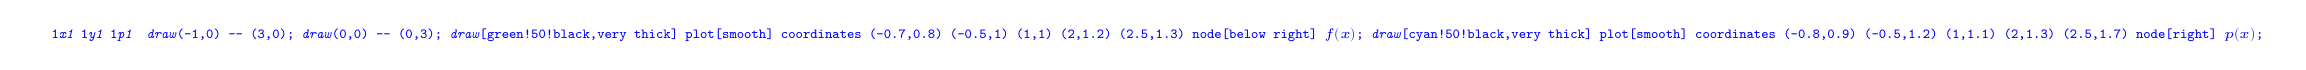
\begin{tikzpicture}

	\draw (-1,0) -- (3,0);
	\draw (0,0) -- (0,3);

	\draw[green!50!black,very thick] plot[smooth] coordinates {(-0.7,0.8) (-0.5,1) (1,1) (2,1.2) (2.5,1.3)}
	node[below right] {$f(x)$};
	\draw[cyan!50!black,very thick] plot[smooth] coordinates {(-0.8,0.9) (-0.5,1.2) (1,1.1) (2,1.3) (2.5,1.7)}
	node[right] {$p(x)$};

	\end{tikzpicture}

	Και μάλιστα:
	\[
	\left|P_n(x)-f(x)\right| \leq \epsilon \quad
	\text{$\epsilon$ δεδομένη ακρίβεια}
	\]

	Όσο το \( \epsilon \) μικραίνει, ο βαθμός του \( P_n(x) \) αυξάνεται.

	Για παράδειγμα, αν έχουμε μερικά σημεία της \( f \):
	\[
	\begin{array}{c|c|c|c|c}
	x_i & 1 & 2 & 3 & 4 \\ \hline
	f(x_i) & 7 & 12 & 21 & 20
	\end{array}
	\]
	ψάχνω ένα πολυώνυμο (κάποιου βαθμού) που να περνάει από αυτά τα
	σημεία.

	\begin{tikzpicture}
	\draw (-1,0) -- (3,0);
	\draw (0,-0.5) -- (0,2);

	\filldraw[cyan] (0.5,0.5) circle (2.5pt)
	(0.9,1) circle (2.5pt)
	(1.5,1.5) circle (2.5pt)
	(2.4,0.7) circle (2.5pt);

	\draw[green!30!black,very thick] plot[smooth,tension=0.7]
	coordinates {(0.1,0,1) (0.5,0.5) (0.9,1) (1.5,1.5) (2.4,0.7) (2.6, 0.2)}
	node[right,scale=0.6] {$p(x)$};						;

	\end{tikzpicture}

	Αν έχω δύο σημεία, το ζητούμενο πολυώνυμο είναι μια ευθεία, δηλαδή
	ένα πολυώνυμο 1\textsuperscript{ου} βαθμού. Για τρία σημεία, θα
	χρειαστώ πολυώνυμο 2\textsuperscript{ου} βαθμού, και γενικά έχω
	ένα μοναδικό
	πολυώνυμο \( n \) βαθμού για \( n+1 \) διακριτά σημεία,
	όπως θα δούμε αργότερα.

	\begin{tikzpicture}[scale=1.3]
	\draw (-1,0) -- (1,0);
	\draw (0,-0.5) -- (0,1.5);


	\filldraw[cyan!50!blue] (-0.5,1) circle (2pt)
	(0,0) circle (2pt)
	(0.5,1) circle (2pt);

	\draw[red!90!blue,very thick] (0,0) -- (0.5,1) --(0.7,1.4);

	\draw[green!30!black,very thick] plot[smooth,tension=0.7]
	coordinates {(-0.5,1) (0,0) (0.5,1)};

	\begin{scope}[xshift=2.5cm]
	\draw (-0.2,0) -- (2,0);
	\draw (0,-0.5) -- (0,1.5);

	\draw[red!90!blue,very thick] (0.1,-0.2) -- (2.2,2.2);

	\draw[green!70!black,thick] plot[smooth,tension=0.7]
	coordinates {(0.25,0) (0.5,0.25) (0.75,1.2)  (1.25,0.8) (1.5,1.45) (2,2)};
	\filldraw[green!50!red] (0.5,0.25) circle (1pt) (1.5,1.45) circle (1pt);
	\end{scope}
	\end{tikzpicture}

	Η πραγματική συνάρτηση μπορεί να έχει διαφορετική συμπεριφορά
	ανάμεσα στα σημεία της τα οποία γνωρίζουμε.

	Στο επόμενο κεφάλαιο θα μάθουμε την προσέγγιση, δηλαδή την εύρεση
	ενός πολυωνύμου συγκεκριμένου βαθμού που να φτάνει κοντά στην
	\( f \), έτσι ώστε να είναι πιο εύκολα υπολογίσιμο αν π.χ. έχουμε
	300 σημεία της συνάρτησης.

	\subsection{Μορφές Αναπαράστασης Πολυωνύμου}
	\paragraph{Εκθετική μορφή}
	\(
	\displaystyle P_n(x) = a_0 + a_1x+a_2x^2 + \dots + a_nx^n
	 \)
	\paragraph{Μορφή κέντρων}
	\(
	\displaystyle P_n(x) = b_0 + b_1(x-c) + b_2(x-c)^2 + \dots
	+ b_n(x-c)^n
	 \)
	\paragraph{Μορφή Newton}
	\(
	\displaystyle P_n(x) = a_0 + a_1(x-c_1) + a_2(x-c_1)(x-c_2)
	+ \dots + a_n(x-c_1)(x-c_2)\cdots(x-c_n)
	= a_0 + \sum_{k=1}^{n} a_k \prod_{i+1}^{k} (x-c_i)
	 \)
	\paragraph{Φωλιασμένη μορφή Newton}
	\begin{align*}
	P_n(x) &= a_0 + (x-c_1)\left[a_1
	+ a_2(x-c_2) + a_3(x-c_2)(x-c_3) + \dots + a_n(x-c_2)\cdots(x-c_n)
	\right] = \dots \\ &= a_0 + (x-c_1)\left[a_1+(x-c_2)
	\left[a_2+ (x-c_3)\left[a_3+\dots + (x-c_{n-1})\left[
	a_{n-1}+(x-c_n)a_n
	\right]\right]\right]
	\right]
	 \end{align*}

	 \paragraph{Μορφή Lagrange}
	 Δεδομένων \( n+1 \) σημείων \( x_0,x_1,\dots,x_n \), έχουμε
	 τα πολυώνυμα:

	 \begin{align*}
	 l_j(x) &= \frac{
	 	(x-x_0)(x-x_1)\cdots(x-x_{j-1})(x-x_{j+1})\cdots(x-x_n)
	 	}{
	 	(x_j-x_0)(x_j-x_1)\cdots(x_j-x_{j-1})(x_j-x_{j+1})
	 	\cdots (x_j-x_n)
	 	} \\
	 	&=
	 	\prod_{\substack{i=0\\i\neq j}}^{n}\frac{(x-x_i)}{(x_j-x_i)}
	 \end{align*}
	 για \( j=0,1,\dots,n \) ονομάζονται \textbf{πολυώνυμα Lagrange} (ο
	 παρονομαστής σταθερός).

	 Παρατηρούμε ότι τα πολυώνυμα είναι φτιαγμένα με τέτοιον τρόπο ώστε:
	 \[
	 l_j(x_i) = \begin{cases}
	 0 & \quad i \neq j \\
	 1 & \quad i = j
	 \end{cases} \ = \delta_{ij}
	 \]

	 Άρα για σταθερές \( a_0,a_1,\dots,a_n \) και σημεία \( x_0,x_1,
	 \dots,x_n \), το πολυώνυμο \[
	 P_n(x) = a_0l_0(x) + a_1l_1(x) + \dots + a_nl_n(x)
	 \]
	 ονομάζεται \textbf{πολυώνυμο σε μορφή Lagrange}.

	 \subsection{Μέθοδοι Παρεμβολής}
	 \begin{gather*}
	    P(x_i) = f(x_i) \\
	 	P(x_i) = \sum_{k=0}^{n} a_kl_k(x_i) = a_i \\[.3ex]
	 	\boxed{P(x) = \sum_{k=0}^n f(x_k)l_k(x)}
	 \end{gather*}

	 \paragraph{Παράδειγμα}
	 Έχουμε τη συνάρτηση:
	 \[
	 \begin{array}{r|c|c|c}
	 i & 0 & 1 & 2 \\ \hline
	 x_i & -1 & 0 & 1 \\ \hline
	 f(x_i) & 1 & 1 & 2
	 \end{array}
	 \]

	 Αναζητώ πολυώνυμο που να παρεμβάλλει την \( f \) σε
	 \begin{enumgreekpar}
	 	\item μορφή Lagrange
	 	\item εκθετική μορφή
	 \end{enumgreekpar}

	 \subparagraph{Λύση}
 	\begin{align*}
 		l_0(x) &=
 		\frac{(x-0)(x-1)}{(-1-0)(-1-1)} = \frac{x(x-1)}{2} \\
 		l_1(x) &=
 		\frac{(x+1)(x-1)}{(0+1)(0-1)} = 1-x^2 \\
 		l_2(x) &= \frac{(x+1)(x-0)}{(1+1)(1-0)} = \frac{x(x+1)}{2} \\
 		\Aboxed{P(x) &= 1l_0(x)+1l_1(x)+2l_2(x)}
 		\quad \leftarrow \text{ μορφή Lagrange}
 		\\ &= \frac{1}{2}x^2 + \frac{1}{2}x + 1
 		\quad \leftarrow \text{ εκθετική μορφή}
 	\end{align*}

 	Ένας άλλος τρόπος θα ήταν να θεωρήσουμε πολυώνυμο
 	2\textsuperscript{ου} βαθμού με 3 άγνωστους συντελεστές, και να λύσω
 	το σύστημα για να τους βρω, κάτι που θα χρησιμεύει αργότερα στην
 	προσέγγιση:
 	\begin{align*}
 	    P(x) &= a_0 + a_1x + a_2x^2 \\
 	    P(-1) &= a_0 - a_1 + a_2 = 1 \\
 	    P(0) &= a_0 = 1 \\
 	    P(1) &= a_0 + a_1 + a_2 = 2
 	\end{align*}

 	\subsubsection{Μέθοδος διηρημένων διαφορών}
 	Η ιδέα είναι να ξεκινάμε από τον μικρό βαθμό, και να χτίζουμε το
 	ζητούμενο πολυώνυμο βαθμό-βαθμό.
 	\begin{align*}
 	P_{k+1}(x) &=
 	\underbrace{a_0+a_1(x-x_0)+\dots+a_k(x-x_0)\cdots(x-x_{k-1})}_{%
 		P_k(x)} + a_{k+1} (x-x_0)\cdots(x-x_k) \\[.4ex]
 	f(x_{k+1}) &= P_{k+1}(x_{k+1})
 	= P_k(x_{k+1}) + a_{k+1}\prod_{i=0}^{k} \left(x_{k+1}-x_i\right) \\
 	a_{k+1} &= \frac{f(x_{k+1}) - P_k(x_{k+1})}{
 		\prod_{i=0}^{k} \left(x_{k+1}-x_i\right)
 		}
 	\end{align*}

 	Για να διευκολύνω τις πράξεις ορίζω:
 	\begin{defn}{Πρώτη Διηρεμένη Διαφορά}{}
 		\[
 		\mathlarger{
 		f\left[x_i,\ x_{i+1}\right] =
 		\frac{f(x_{i+1})-f(x_i)}{x_{i+1}-x_i}
 	    }
 		\]
 	\end{defn}

 	Η \( k \)-οστή Διηρεμένη Διαφορά είναι:
 	\begin{defn}{k-οστή Διηρεμένη Διαφορά}{}
 		\[
 		\mathlarger{
 			f\left[x_i,\ x_{i+1}, \dots,\ x_{i+k}\right] =
 			\frac{
 				f[x_{i+1},x_{i+2},\dots,x_{i+k}]
 				- f[x_i,x_{i+1},\dots,x_{i+k-1}]
 				}{x_{i+k}-x_i}
 		}
 		\]
 	\end{defn}

 	Για διευκόλυνσή μας, αντί να χρησιμοποιούμε τους τύπους, μπορούμε
 	να χρησιμοποιήσουμε τον Πίνακα Διηρημένων Διαφορών.

 	\paragraph{Πίνακας ΔΔ}
 	\[
 	\begin{array}{llllll}
 	 & & 1^{\text{η}} & 2^\text{η} & 3^\text{η} & 4^\text{η}\\
 	x_0 & f(x_0) & f[x_0,x_1] & = \frac{f(x_1)-f(x_0)}{x_1-x_0} & \\
 	x_1 & f(x_1) & f[x_1,x_2] & f[x_0,x_1,x_2] & =
 	\frac{f[x_1,x_2]-f[x_0,x_1]}{x_2-x_0} \\
 	x_2 & f(x_2) & f[x_2,x_3] & f[x_1,x_2,x_3] & f[x_0,x_1,x_2,x_3] &
 	=\frac{f[x_1,x_2,x_3]-f[x_0,x_1,x_2]}{x_3-x_0} \\
 	x_3 & f(x_3) & f[x_3,x_4] & f[x_2,x_3,x_4] & f[x_1,x_2,x_3,x_4]
 	& f[x_0,x_1,x_2,x_3,x_4]
 	\\
 	x_4 & f(x_4) & &
 	\end{array}
 	\]

 	Τότε το πολυώνυμο θα είναι:
 	\begin{align*}
 		P_k(x) &= f(x_0) + f[x_0,x_1](x-x_0) +
 		f[x_0,x_1,x_2](x-x_0)(x-x_1)
 		\\ & + \dots +
 		f[x_0,x_1,\dots,x_k](x-x_0)(x-x_1)\cdots(x-x_{k-1})
 	\end{align*}

 	\paragraph{Παράδειγμα}
 	\hspace{0pt}

 	\begin{tabular}{|c|c|c|c|c|}
 		\hline
 		\(i\) & 0 & 1 & 2 & 3 \\
 		\hline
 		\(x_i\) & 0 & 1 & 2 & 4 \\
 		\hline
 		\(f(x_i)\) & 1 & 1 & 2 & 5 \\
 		\hline
 	\end{tabular}

 	Πίνακας ΔΔ:
 	\[
 	\begin{array}{ccccc} \cline{2-2}
 	0 & \multicolumn{1}{|c|}{1 \searrow} & & &  \\ \cline{2-3}
 	& & \multicolumn{1}{|c|}{\frac{1-1}{1-0} \searrow} & & \\ \cline{3-4}
 	1 & 1 \nesearrow & &
 	\multicolumn{1}{|c|}{\frac{1}{2} \searrow} & \\ \cline{4-5}
 	& & 1 \nesearrow & & \multicolumn{1}{|c|}{-\frac{1}{12}}\\ \cline{5-5}
 	2 & 2 \nesearrow & & \frac{1}{6} \nearrow & \\
 	& & \frac{3}{2} \nearrow & & \\
 	4 & 5 \nearrow & & &
 	\end{array}
 	\]

 	Άρα:
 	\begin{align*}
 	P_3(x) &= 1 + 0(x-0) + \frac{1}{2}(x-0)(x-1)-\frac{1}{12}
 	(x-0)(x-1)(x-2) \\ &= \frac{1}{12} (-x^3+9x^2-8x+12)
 	\end{align*}

 	\begin{tikzpicture}
 	\begin{axis}[grid=both,ymin=0,ymax=10,xmax=7,xmin=-3,xticklabel=\empty,yticklabel=\empty,
 	minor tick num=1,axis lines = middle,xlabel=$x$,ylabel=$y$,label style =
 	{at={(ticklabel cs:1.1)}}]
 	\addplot[blue,thick,samples=50,domain=-3:7] {1/12*(-x^3+9*x^2-8*x+12)};

 	\filldraw [fill=gray!30, draw=black, thick] (axis cs:0,1) circle [radius=3pt];
 	\filldraw [fill=gray!30, draw=black, thick] (axis cs:1,1) circle [radius=3pt];
 	\filldraw [fill=gray!30, draw=black, thick] (axis cs:2,2) circle [radius=3pt];
 	\filldraw [fill=gray!30, draw=black, thick] (axis cs:4,5) circle [radius=3pt];

 	% nice node: node [label={[inner sep=1pt, fill=white,text=black, fill opacity=0.75, text opacity=1]above left:$(65, 35)$}] {};

 	\end{axis}
 	\end{tikzpicture}

 	\subsubsection{Μέθοδος πεπερασμένων διαφορών}
 	Για τη μέθοδο αυτή, θεωρούμε ότι τα σημεία της \( f \)
 	που έχουμε ισαπέχουν μεταξύ τους:
 	\begin{gather*}
 		x_0,x_1,\dots,x_n \ \in [a,b] \\
 		x_i = x_0 + ih \quad \text{όπου } h=\frac{b-a}{n}
 		\\[.4ex]
 		f\left[x_i,x_{i+1}\right] =
 		\frac{f(x_{i+1})-f(x_i)}{h}
 	\end{gather*}

 	Ορίζω συμβολισμούς για ευκολία:
 	\begin{align*}
 		\Delta^0 f(x_i) &= f(x_i) \\
 		\Delta^1 f(x_i) &=
 		f(x_{i+1}) - f(x_i) = f(x_i+h) - f(x_i) \\
 		\vdots \\
 		\Delta^k f(x_i) &=
 		\Delta \left(\Delta^{k-1}\left(f(x_i)\right)\right)
 		= \Delta^{k-1} f(x_{i+1}) - \Delta^{k-1} f(x_i)
 	\end{align*}

 	\begin{defn}{k-οστή πεπερασμένη διαφορά}{}
 		\[
 			f\left[x_i,x_{i+1},\dots,x_{i+k}\right]
 			= \frac{\Delta^k f(x_i)}{k! h^k}
 			\qquad \text{προκύπτει μετά από πράξεις}
 		\]
 	\end{defn}

 	Άρα το πολυώνυμο γίνεται:
 	\begin{align*}
 	P_n(x) &= f(x_0) + f[x_0,x_1](x-x_0) + \dots
 	\\ & \quad \dots +
 	f[x_0,x_1,\dots,x_n](x-x_0)(x-x_1)\dots(x-x_{n-1})
 	\\ &= f(x_0) + \frac{\Delta^1 f(x_0)}{1!h^1}(x-x_0)
 	+ \frac{\Delta^2 f(x_0)}{2!h^2}(x-x_0)(x-x_1) + \dots \\
 	& \quad \dots + \frac{\Delta^n f(x_n)}{n!h^n}
 	(x-x_0)(x-x_1)\cdots
 	(x-x_{n-1})
 	\end{align*}

 	Θα βρούμε μια διαδικασία ώστε να υπολογίζουμε το πολυώνυμο
 	γρηγορότερα. Αν \( x = x_0+rh \), αποδεικνύεται πως
 	(οι πράξεις υπάρχουν στο βιβλίο):
 	\[
 	\mathlarger{
 		\boxed{
 			P_n(x_0+rh) = \sum_{i=0}^{n}
 			\left(\begin{matrix}
 			r\\i
 			\end{matrix}\right)
 			\Delta^i f(x_0)
 			}
 		}
 	\]
 	όπου \( \displaystyle \binom{r}{i} =
 	\frac{r(r-1)\cdots\left(r-(i-1)\right)}{i!} \)

 	\paragraph{Παράδειγμα}
 	\hspace{0pt}

 	\begin{tabular}{|c|c|c|c|c|c|}
 		\hline
 		\(i\) & 0 & 1 & 2 & 3 & 4\\
 		\hline
 		\(x_i\) & 1 & 2 & 3 & 4 & 5\\
 		\hline
 		\(f(x_i)\) & 1 & -1 & 1 & -1 & 1\\
 		\hline
 	\end{tabular}

 	\[
 		\begin{array}{|c|c|c|c|c|c|}
 			\hline
 			 x_0   & f(x_0) \searrow &                 &                 &                 &  \\ \hline
 			       &        & \Delta^1 f(x_0) \searrow &                 &                 &  \\ \hline
 			 x_1   & f(x_1) \nesearrow &                 & \Delta^2 f(x_0) \searrow &                 &  \\ \hline
 			       &        & \Delta^1 f(x_1) \nesearrow &                 & \Delta^3 f(x_0) \searrow &  \\ \hline
 			 x_2   & f(x_2) \nesearrow &                 & \Delta^2 f(x_1) \nesearrow &                 & \Delta^4 f(x_0) \\ \hline
 			       &        & \Delta^1 f(x_2) \nesearrow &                 & \Delta^3 f(x_1) \nearrow &  \\ \hline
 			 x_3   & f(x_3) \nesearrow &                 & \Delta^2 f(x_2) \nearrow &                 &  \\ \hline
 			       &        & \Delta^1 f(x_3) \nearrow &                 &                 &  \\ \hline
 			 x_4   & f(x_4) \nearrow &                 &                 &                 &  \\ \hline
 			\vdots &        &                 &                 &                 &  \\ \hline
 		\end{array}
 	\]
 	όπου τα στοιχεία \( \Delta^1 f(x_0), \ \Delta^2 f(x_0),\ \dots \) είναι ίσα
 	με \textbf{τη διαφορά των δύο προηγούμενων στοιχείων}, δηλαδή:
 	\begin{align*}
 		\Delta^1 f(x_0) &= f(x_1) - f(x_0) \\
 		\Delta^1 f(x_1) &= f(x_2) - f(x_1) \\
 		\Delta^1 f(x_2) &= f(x_3) - f(x_2) \\
 		\Delta^2 f(x_0) &= \Delta^1 f(x_1) - \Delta^1 f(x_0)
 		\\ \text{κλπ.}
 		\intertext{και γενικά:}
 		\Delta^k f(x_i) &= \Delta^{k-1} f(x_{i+1}) - \Delta^{k-1} f(x_i)
 	\end{align*}

 	\[
 	\begin{array}{cccccc}
 		\cellcolor{blue!25}1 & \cellcolor{blue!25} 1 \searrow &                                 &                                &                                &  \\
 		                     &                                & \cellcolor{blue!25} -2 \searrow &                                &                                &  \\
 		         2           &         -1 \nesearrow          &                                 & \cellcolor{blue!25} 4 \searrow &                                &  \\
 		                     &                                &          2 \nesearrow           &                                & \cellcolor{blue!25}-8 \searrow &  \\
 		         3           &          1 \nesearrow          &                                 &         -4 \nesearrow          &                                & \cellcolor{blue!25}1 \\
 		                     &                                &          -2 \nesearrow          &                                &           8 \nearrow           &  \\
 		         4           &         -1 \nesearrow          &                                 &           4 \nearrow           &                                &  \\
 		                     &                                &           2 \nearrow            &                                &                                &  \\
 		         5           &           1 \nearrow           &                                 &                                &                                &
 	\end{array}
 	\]

 	\begin{align*}
 		P_4(1+r) &= 1-2\binom{r}{1}+4\binom{r}{2}-8\binom{r}{3}
 		+6\binom{r}{4}
 		\intertext{όπου \( x = x_0+rh \implies
 			r=1.5 \text{ για } x = 2.5 \)}
 		\\
 		P(2.5) &= 1 -2 \binom{1.5}{1} + 4\binom{1.5}{2}
 		-8\binom{1.5}{3} + 16\binom{1.5}{4}
 	\end{align*}

 	\subsubsection{Μέθοδος Aitken}
 	Έστω \( p,q \) δύο πολυώνυμα παρεμβολής μικρότερου
 	βαθμού (για \( m+2 \) σημεία),
 	και \( r \) το πολυώνυμο παρεμβολής για όλα
 	τα σημεία (\( m+3 \) σημεία) \( \qquad x_0,x_1,\dots,
 	x_m,y,z \), και γνωρίζω:
 	\begin{itemize}
 		\item \( p(x_i)=q(x_i)=r(x_i)=f(x_i)
 		\text{ για } i=0,1,\dots,m \)
 		\item \( p(y) = r(y) = f(y) \)
 		\item \( q(z) = r(z) = f(z) \)
 	\end{itemize}

 	Τότε η \( r(x) \) που είναι η συνάρτηση που θέλω να
 	παρεμβάλλει την \( f \) είναι:
 	\[
 	\boxed{
 	r(x) = \frac{(y-x)q(x) - (z-x)p(x)}{y-z}
    }
 	\]

 	\paragraph{}
 	Έστω \( A_{k,r} \) η τιμή στο \( \bar x \) του πολυωνύμου
 	παρεμβολής της \( f(x) \) στα σημεία \( x_0,x_1,
 	\dots,x_{k-1},x_r \):
 	\begin{align*}
 	A_{k,r} &= f[x_0] + f[x_0,x_1](\bar x-x_0)
 	+ f[x_0,x_1,x_2](\bar x-x_0)(\bar x-x_1) + \dots
 	\\ &\quad \dots + f[x_0,x_1,\dots,x_k](\bar x-x_0)
 	(\bar x-x_1)\cdots(\bar x-x_{k-1}) \\
 	A_{k,r} &= \frac{(x_{k-1}-\bar x)A_{k-1,r}
 		-(x_r-\bar x)A_{k-1,k-1}}{x_{k-1}-x_r}
	\end{align*}


	\begin{tikzpicture}
	\begin{scope}[yscale=-0.6,xscale=1]
	\foreach \i in {0,1,...,4} {
		\draw (0,\i) node {$x_\i$};
		\draw (1,\i) node {$A_{0,\i}$};
		\draw (7,\i) node {$x_\i - \bar x$};
	}

	\foreach \i in {1,...,4} {
		\draw (2,\i-0.5) node {$A_{1,\i}$};
	}

	\foreach \i in {2,...,4} {
		\draw (3,\i-1) node {$A_{2,\i}$};
	}

	\foreach \i in {3,...,4} {
		\draw (4,\i-1.5) node {$A_{3,\i}$};
	}

	\foreach \i in {4,...,4} {
		\draw (5,\i-2) node {$A_{4,\i}$};
	}

	\end{scope}
	\end{tikzpicture}


	\paragraph{π.χ.}
	\begin{align*}
		A_{2,3} &=
		\frac{(x_1-\bar x)A_{1,3}-(x_3-\bar x)A_{1,1}}{x_1-x_3}
	\end{align*}

	\subsection{Ασκήσεις}
	\paragraph{Άσκηση}
	Να βρεθεί πολυώνυμο Lagrange που να παρεμβάλλει την
	\( \mathlarger{f(x)=e^x} \) στα σημεία \( x_0=-1,\ x_1=0,\ x_2=1 \).
	\subparagraph{Λύση}
	Θυμόμαστε ότι το πολυώνυμο Lagrange δίνεται από τους τύπους:
	\begin{align*}
	P_n(x) &= l_0(x)f(x_0)+l_1(x)f(x_1)+l_2(x)f_2(x_2) \\
	l_0(x) &= \frac{(x-x_1)(x-x_2)}{(x_0-x_1)(x_0-x_2)}
	= \frac{(x-0)(x-1)}{(-1)(-2)} = \frac{1}{2}(x^2 - x) \\
	l_1(x) &= \frac{(x-x_0)(x-x_2)}{(x_1-x_0)(x_1-x_2)}
    = \frac{(x+1)(x-1)}{1\cdot (-1)} = -x^2+1 \\
    l_2(x) &= \frac{(x-x_0)(x-x_1)}{(x_2-x_0)(x_2-x_1)} = \frac{1}{2}
    (x^2+x)
    \intertext{Άρα}
    P_2(x) &= \frac{1}{2e}(x^2-x)+ (-x^2+1) + \frac{e}{2}(x^2+x)
    \\ &=
    \left(1+\frac{e}{2}+\frac{1}{2e}\right)x^2
    +\left(\frac{e}{2}-\frac{1}{2e}\right)x -1
    \quad \text{(δεν είναι απαραίτητο να το φτάσουμε μέχρι εδώ)}
	\end{align*}

	\begin{tikzpicture}[scale=.8]
	\begin{axis}[samples=30,very thick,domain=-1.5:1.5,no marks,grid=both,axis lines = middle,clip=false]
	\addplot+{e^x} node[above right] {$e^x$};
	\addplot+{(x^2-x)/(2*e) + (1-x^2) + (e/2)*(x^2+x) }
	node[above right] {$P_2(x)$};

	\filldraw [fill=red!50!gray!30, draw=black, thick, fill opacity=.7]
	(axis cs:-1,1/e) circle [radius=3pt] (axis cs:0,1) circle [radius=3pt] (axis cs:1,e) circle [radius=3pt];
	\end{axis}
	\end{tikzpicture}

	\paragraph{Άσκηση}
	Να βρεθεί πολυώνυμο Newton που να παρεμβάλλει την παρακάτω \( f \)
	με τη μέθοδο διηρημένων διαφορών:
	\[
	f(-1) = 1,\quad f(1) = 2 \quad \text{και} \quad f(2)=-1
	\]
	\subparagraph{Λύση}
    \[
    \begin{array}{cccc}
    x_i&f(x_i)&1\textsuperscript{η}&2\textsuperscript{η} \\
    -1 & 1 \searrow & &  \\
    & & \frac{1}{2} \searrow & \\
    1 & 2 \nesearrow & & \frac{-3-\sfrac{1}{2}}{2-(-1)} = -\frac{7}{6} \\
    & & -3 \nearrow & \\
    2 & -1 \nearrow
    \end{array}
    \]
	\[
	P_2(x) = 1 + \frac{1}{2}(x+1) - \frac{7}{6}(x+1)(x-1)
	\]

	\paragraph{Άσκηση}
	Να βρεθεί η τιμή \( f(0.5) \) (intrapolation)
	χρησιμοποιώντας τη μέθοδο πεπερασμένων διαφορών. Δίνεται ο πίνακας
	τιμών της \( f \)
	\[
	\begin{array}{r|c|c|c|c|c}
	x_i & 0 & 1 & 2 & 3 & 4 \\ \hline
	f(x_i) & 1 & 0 & -1 & 1 & 2
	\end{array}
	\]
	\subparagraph{Λύση}
	Οι τύποι για τις \( k \)-οστές διαφορές θα δίνονται στις εξετάσεις,
	αλλά είναι πιο κομψό και εύκολο να χρησιμοποιήσουμε τον πίνακα:

	\[
	\begin{array}{cccccc}
		x_i & f(x_i) & & & & \\
		\cellcolor{blue!25}0 & \cellcolor{blue!25} 1 \searrow & &     &     &\\
		&     & \cellcolor{blue!25} -1 \searrow &     & &\\
		1   &   0 \nesearrow& & \cellcolor{blue!25} 0 \searrow & &\\
		& &-1 \nesearrow   & & \cellcolor{blue!25}3 \searrow &\\
		2   &-1 \nesearrow& &   3 \nesearrow&& \cellcolor{blue!25}-7 \\
		&&2 \nesearrow&&   -4 \nearrow   &\\
		3   &   1 \nesearrow& &   -1 \nearrow   &&\\
		&&   1 \nearrow&&&\\
		4   &   2 \nearrow   & &&&
	\end{array}
    \]

	\begin{align*}
	P_4(\overset{\mathclap{\substack{x=x_0+rh\\\uparrow}}}{x}) &=
	    f(x_0) + \binom{r}{1}\Delta f(x_0) + \binom{r}{2}\Delta^2 f(x_0)
	    + \binom{r}{3}\Delta^3 f(x_0) + \binom{r}{4} \Delta^4 f(x_0)
	\intertext{\( 0.5 = 0 + r\cdot 1 \implies r=0.5 \)}
    &= 1-\binom{0.5}{1}+0\binom{0.5}{2}+3\binom{0.5}{3}-7\binom{0.5}{4}
    = 0.9609375
    \intertext{όπου
    	\( \binom{r}{k} = \frac{r(r-1)\cdots\left(r-(k-1)\right)}{k!} \)
    	}
	\end{align*}

	\paragraph{Άσκηση}
	Να βρεθεί η τιμή του πολυωνύμου παρεμβολής \( P(5) \) για τα σημεία
	\( x_i \) και τις αντίστοιχες τιμές της συνάρτησης \( f(x_i) \) που
	δίνονται στον πίνακα με τη μέθοδο Aitken:
	\[
	\begin{array}{r|cccc}
	x_i & 2 & 4 & 6 & 8 \\ \hline
	f(x_i) & 1 & -2 & 3 & 5
	\end{array}
	\]
	\subparagraph{Λύση}
	\begin{align*}
		x_i - \underbrace{\bar x}_{5} & \\
		2-5 &= -3 \\ 4-5 &= -1 \\ 6-5 &= 1 \\ 8-5 &= 3
	\end{align*}


\begin{tikzpicture}[scale=1]
\def\fs{22pt}
\draw (0,0) node{$8$};
\draw (0,\fs) node {$6$};
\draw (0,2*\fs) node {$4$};
\draw (0,3*\fs) node {$2$};

\draw[green!70!black] (0,3*\fs) circle (7pt);
\draw[green!70!black] (0,2*\fs) circle (7pt);
\draw[thick,cyan!70!black] (0,2*\fs) circle (9pt);
\draw[thick,cyan!70!black] (0,1*\fs) circle (8pt);

\draw (0.9,0) node {$5$};
\draw (0.9,1*\fs)
node[thick,draw=cyan!70!black,shape=rectangle] {$-3$};
\draw (0.9,2*\fs) node[draw=green!70!black,minimum width=6mm,shape=rectangle] {$-2$};
\draw (0.9,2*\fs)
node[thick,draw=cyan!70!black,minimum width=9mm,minimum height=7mm,shape=rectangle] {$\phantom{-2}$};
\draw (0.9,3*\fs) node[draw=green!70!black,minimum width=6mm,shape=rectangle] {$1$};

\draw[->,green!70!black] (1.2,3*\fs+2mm) -- ++(1.5,0) node[right,scale=.7] {$\cdot (-3)$} -- ++(0,-2.5mm);
\draw[->,green!70!black] (1.3,2*\fs+2mm) -- ++(0,0.4) -- ++(0.7,0)
node[above left,scale=.6,yshift=-1mm] {$\cdot(-1)$};
\draw[->,cyan!70!black] (1.35,2*\fs+2mm) -- ++(0.3,0) -- ++(0,-0.4)
node[below,scale=.6,xshift=1mm] {$\cdot(-1)$} -- ++(0.35,0);
\draw[->,cyan!70!black] (0.9,1*\fs-3mm) -- ++(0,-2mm) -- ++(1.1,0)
node[below left,scale=.7] {$\cdot 1$};

\draw (2.5,2.5*\fs) node[right,xshift=-5mm,scale=0.5] {$\frac{(-2)(-3)-(-1)\cdot1}{2-4}=$};
\draw (3.8,2.5*\fs) node {$-\frac{7}{2}$};
\draw (2.5,1.5*\fs) node[right,xshift=-2mm,scale=0.5] {$\frac{3\cdot(-3)-(1)\cdot1}{2-6}=$};
\draw (3.8,1.5*\fs) node {$\frac{5}{2}$};
\draw (2.5,0.5*\fs) node[right,xshift=0mm,scale=0.5] {$\frac{5\cdot(-3)-1\cdot3}{2-8}=$};
\draw (3.8,0.5*\fs) node {$3$};
\draw (2,2.1*\fs) rectangle (4.2,2.9*\fs);
\draw (2,1.1*\fs) rectangle (4.2,1.9*\fs);
\draw (2,0.1*\fs) rectangle (4.2,0.9*\fs);

\draw (5.2,1*\fs) node[draw,rectangle,minimum width=12mm,yshift=-1mm] {$-\frac{1}{2}$};
\draw (5.2,2*\fs) node[draw,rectangle,minimum width=12mm,yshift=1mm] {$-\frac{15}{8}$};

\draw (6.2,1.5*\fs) node[right,scale=0.5,xshift=1mm,yshift=1mm]
{$\frac{-\frac{15}{8}\cdot1-\left(-\frac{1}{2}\right)\cdot3}{6-8}=$};
\draw (7.9,1.5*\fs) node {$\frac{3}{16}$};
\draw (6.2,1.1*\fs) rectangle (8.2,1.9*\fs);

\draw[->] (9,-0.2) node[below] {Λύση $p(5)$} -- (8,0.7);
\end{tikzpicture}

	Άρα \( P(5) = \frac{3}{16} \), λύση που φαίνεται λογική, αφού
	βρίσκεται ανάμεσα στο -2 και το 3.


	\section{Προσέγγιση}
	Η προσέγγιση μοιάζει με την παρεμβολή, με τη διαφορά ότι δεν
	επιθυμούμε το πολυώνυμο που βρούμε να περνάει από όλα τα σημεία της
	αρχικής συνάρτησης, αλλά να έχει την ελάχιστη απόσταση από αυτά. Το
	κέρδος μας με αυτόν τον τρόπο είναι ότι το πολυώνυμο που θα βρούμε
	είναι μικρότερου βαθμού.

	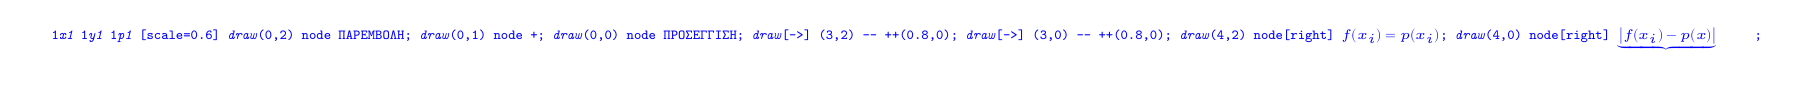
\begin{tikzpicture}[scale=0.6]
	\draw (0,2) node {ΠΑΡΕΜΒΟΛΗ};
	\draw (0,1) node {+};
	\draw (0,0) node {ΠΡΟΣΕΓΓΙΣΗ};

	\draw[->] (3,2) -- ++(0.8,0);
	\draw[->] (3,0) -- ++(0.8,0);

	\draw (4,2) node[right] {$f(x_i) = p(x_i)$};
	\draw (4,0) node[right] {$
		\underbrace{\left|f(x_i)-p(x)\right|}_{
			\mathclap{\text{πολυώνυμο μικρότερου βαθμού}}}$
		ελάχιστη};
	\end{tikzpicture}

	\paragraph{}
	Έστω οι τιμές μιας συνάρτησης:
	\[
	\begin{array}{r|c|c|c|c}
	x_i & x_0 & x_1 & \dots & x_{m-1} \\ \hline
	f(x_i) & f(x_0) & f(x_1) & \dots & f(x_{m-1})
	\end{array}
	\]

	
\begin{tikzpicture}[scale=1]
	\draw (-0.5,0) -- (3,0);
	\draw (0,-0.5) -- (0,3);

	\draw[thick,blue!50!black,mark position=0.8(a)] (-1,2) -- ++(15:4);
	\draw[thick,blue!50!black,mark position=0.1(b)] (0.5,-0.5) -- ++(70:3);
	\draw[thick,blue!50!black,mark position=0.9(c)] (-1,-0.5) -- ++(30:5);

	\draw[<-,cyan] (a) -- ++(-40:0.5) node[below,rotate=30] {κακή προσέγγιση};
	\draw[<-,cyan] (b) -- ++(-40:0.5) node[below,rotate=20] {μέτρια προσέγγιση};
	\draw[<-,cyan] (c) -- ++(-40:0.5) node[below,rotate=30] {καλύτερη προσέγγιση};

	\filldraw (0.3,0.3) circle (1pt) (0.4,0.5) circle (1pt) (0.8,0.6) circle (1pt)
	(rand,rand) circle (1pt) (0.7,2) circle (1pt) (1,1.5) circle (1pt)
	(1.5,1) circle (1pt) (2,1.2) circle (1pt) (2.5,1) circle (1pt);

	\end{tikzpicture}

	Αν ζητάμε η προσέγγιση \( P(x) \) να είναι μια ευθεία, τότε στην
	ιδανική περίπτωση:
	\[
	P(x_i) = a_0 + a_1x_i = f(x_i) \quad \forall x_i
	\]
	τότε έχουμε ένα σύστημα:
	\[
	\left[
	\begin{matrix}
	1 & x_0 \\ 1 & x_1 \\ 1 & x_2 \\ \vdots & \vdots \\ 1 & x_{m-1}
	\end{matrix}
	\right] \left[
	\begin{matrix}
	a_0 \\ a_1
	\end{matrix}
	\right] = \left[
	\begin{matrix}
	f(x_0) \\ f(x_1) \\ f(x_2) \\ \vdots \\ f(x_{m-1})
	\end{matrix}
	\right]
	\]
	που είναι σύστημα 2 αγνώστων αλλά \( m \) εξισώσεων, κάτι που μάλλον
	θα είναι αδύνατο.

	Επομένως αντί να λύσω την εξίσωση:
	\[
	Ax = b
	\]
	θα λύσω την:
	\[
	A\bar x \simeq b
	\]
	με σκοπό να ελαχιστοποιήσω την απόσταση (υπόλοιπο):
	\[
	A\bar x -b.
	\]

	Η παραπάνω σχέση όμως δεν εκφράζει έναν αριθμό, αλλά έναν πίνακα!
	Για να "ελαχιστοποιήσουμε" αυτόν τον πίνακα θα ορίσουμε κάποια
	μεγέθη.

	\subsection{Στοιχεία Αριθμητικής Γραμμικής Άλγεβρας}
	\subsubsection{Εσωτερικό γινόμενο}
	\textit{Εσωτερικό γινόμενο} σε χώρο \( V \) είναι μια \textbf{πράξη}
	για κάθε \( x,y \in V \)
	(συμβολίζεται με \( (x,y) \) ή \( \langle x,y \rangle \))
	ορίζει έναν \textbf{αριθμό} που ικανοποιεί:
	\begin{enumroman}
		\item \( (x,x) \geq 0 \), ισότητα μόνο αν \( x=0 \)
		\item \( (x,y) = (y,x) \quad \forall x,y\in V \)
		\item \( (ax+by,z) = a(x,z)+b(y,z) \)
	\end{enumroman}

	Πιο συγκεκριμένα, για κάποιους χώρους ορίζουμε:
	\begin{align*}
	\mathbb R^n &: \ (x,y) = x^{\mathrm T}y \quad
	\text{για } x,y \in \mathbb R^n
	\\
	\mathbb R^{m\times n} &: (A,B) =
	\sum_{i=1}^{m}\sum_{j=1}^{n} a_{ij}b_{ij}
	\end{align*}

	Για συναρτήσεις, έχουμε \( (f,g) = \int f(x)g(x)\dif x \)

	Δύο διανύσματα \( x,y \in V \) λέγονται \textbf{ορθογώνια} όταν
	\( (x,y) = 0\), και γράφουμε \( x \perp y \).

	\subsubsection{Μήκος - Νόρμα (norm) διανύσματος}
	Ως νόρμα μπορούμε να επιλέξουμε οποιαδήποτε συνάρτηση που καλύπτει
	κάποια αξιώματα (για παράδειγμα, νόρμα ενός διανύσματος μπορεί να
	είναι το μέγιστο στοιχείο ενός διανύσματος).

	Ένας χώρος \( V \) είναι εφοδιασμένος με \textbf{μήκος} ή
	\textbf{νόρμα} αν για κάθε \( x \in V \) υπάρχει αριθμός
	\( \Vert x\Vert \) που ικανοποιεί:

	\begin{enumroman}
		\item \( \Vert x\Vert > 0 \) με ισότητα μόνο εάν \( x=0 \)
		\item \( \Vert ax\Vert = |a|\,\Vert x\Vert \) για κάθε σταθερά \( a \)
		\item \( \Vert x+y\Vert \leq \Vert x\Vert+\Vert y\Vert \ \forall x,y\in V  \)
	\end{enumroman}

	\paragraph{Είδη νορμών}
	Για ένα διάνυσμα \( x=(x_1,x_2,\dots,x_n)^{\mathrm T} \)
	\begin{align*}
		l_{\infty} &: \Vert x\Vert _{\infty} = \max_{1\leq i \leq n}|x_i|
		\qquad \text{ (άπειρη νόρμα)}
		\\
		l_p &: \Vert x\Vert _{p} =
		\left(\sum_{i=1}^n |x_i|^p\right)^{\frac{1}{p}}
		\quad \text{ ($p$-οστή νόρμα)}
		\\
		l_2 &: \Vert x\Vert _2 = \sqrt{x^{\mathrm T}x} =
		\sqrt{x_1^2 + \dots + x_n^2}
		\quad \text{ (ευκλείδια νόρμα)}
	\end{align*}

	\paragraph{Απόσταση}
	μεταξύ διανυσμάτων \( x,y \in \mathbb R  \) είναι ο αριθμός:
	\[
    \mathlarger{\Vert x-y\Vert }
	\]

	\paragraph{Θεωρήματα}
	\[
	\Vert x+y\Vert ^2 = \Vert x\Vert ^2 + \Vert y\Vert ^2
	\]

	Cauchy-Schwartz:
	\[
	\left\Vert(x,y)\right\Vert \leq \Vert x\Vert \,\Vert y\Vert
	\]

	\subsubsection{Ορθογώνιοι Υποχώροι}
	\begin{defn}{Ορθογώνιοι Υποχώροι}{}
		Δύο υποχώροι \( X,Y \) του  \( \mathbb R^n \) λέγονται
		\textbf{ορθογώνιοι}, αν \( x^{\mathrm T}y = 0 \) \textbf{για
		κάθε} \( x \in X \) και \( y \in Y \).

	    Γράφουμε: \( \mathlarger{X \perp Y} \)
	\end{defn}
	\begin{defn}{Ορθογώνιο Συμπλήρωμα}{}
		Το σύνολο:
		\[
		\mathlarger{
			Y^\perp
			} = \left\lbrace
			x \in \mathbb R^n : x^{\mathrm T}y = 0 \quad
			\forall y \in Y
			 \right\rbrace
		\]
		είναι το \textbf{ορθογώνιο συμπλήρωμα} του \( Y \).

		Για παράδειγμα, το ορθογώνιο συμπλήρωμα του πίνακα στην αίθουσα
		Α3 είναι ο κάθετος τοίχος.
	\end{defn}
	\begin{defn}{}{}
		Για \( A \in \mathbb R^{m \times n} \):
		\begin{itemize}
			\item \textbf{Μηδενοχώρος} του \( A \):
			\( \mathrm N(A) = \left\lbrace x\in\mathbb R^n: Ax=0
			 \right\rbrace \)
			\item \textbf{Χώρος των στηλών} του \( A \):
			\( \mathrm R(A)  = \left\lbrace
			b \in \mathbb R^m: b = Ax \text{ για }
			x \in \mathbb R^n \right\rbrace
			\)
			\item \textbf{Χώρος των γραμμών} του \( A \):
			\( \mathrm R(A^{\mathrm T}) = \left\lbrace
			y \in \mathbb R^n: y = A^{\mathrm T}x \text{ για }
			x \in \mathbb R^m
			 \right\rbrace \)
		\end{itemize}
	\end{defn}
	\begin{theorem}{Θεμελιώδες Θεώρημα Γραμμικής Άλγεβρας}{}
		\begin{align*}
			\mathlarger{N(A)} &\mathlarger{= R(A^{\mathrm T})^\perp}
			\\
			\mathlarger{N(A^{\mathrm T})} &\mathlarger{= R(A)^\perp}
		\end{align*}
	\end{theorem}

    \subsection{Πίσω στο αρχικό πρόβλημα}
    Ορίζω:
    \begin{align*}
    \text{διαφορά } r(x) &= b - Ax \\
    \left\Vert r(x)\right\Vert &= \Vert b-Ax\Vert
    \end{align*}

    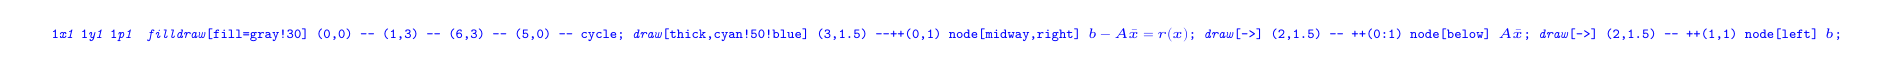
\begin{tikzpicture}
    \filldraw[fill=gray!30] (0,0) -- (1,3) -- (6,3) -- (5,0) -- cycle;

    \draw[thick,cyan!50!blue] (3,1.5) --++(0,1) node[midway,right] {$b-A\bar x=r(x)$};
    \draw[->] (2,1.5) -- ++(0:1) node[below] {$A\bar x$};
    \draw[->] (2,1.5) -- ++(1,1) node[left] {$b$};
    \end{tikzpicture}


    Το διάνυσμα \( r(x) \) ανήκει στο ορθογώνιο συμπλήρωμα του χώρου
    των στηλών, άρα στο μηδενοχώρο του \( A^{\mathrm T} \) (από το
    Θεμελιώδες Θεώρημα Γραμμικής Άλγεβρας), επομένως:

    \begin{align*}
    	A^{\mathrm T} r(x) &= 0 \\
    	A^{\mathrm T} (b-A\bar x) &= 0
    \end{align*}

    Άρα: \[
    \boxed{
    \mathlarger{\mathlarger{\mathlarger{
    		Α^{\mathrm T}Ax = A^{\mathrm T}b
    	}}}} \quad \xleftarrow{\hspace{5pt}} \text{ κανονικές εξισώσεις}
    \]

    \paragraph{Παράδειγμα}
    Να προσεγγιστεί η \( f(x) \) με πολυώνυμο πρώτου βαθμού, όπου:
    \[
    \begin{array}{r|ccc}
    x_i & 0 & 3 & 6 \\ \hline
    f(x_i) & 1 & 4 &  5
    \end{array}
    \]

    \subparagraph{Λύση}
    \[
    A = \left[ \begin{matrix}
    1 & 0 \\ 1 & 3 \\ 1 & 6
    \end{matrix} \right], \quad x = \left[ \begin{matrix}
    a_0 \\ a_1
    \end{matrix}\right], \quad b = \left[\begin{matrix}
    1 \\ 4 \\ 5
    \end{matrix} \right]
    \]

    \begin{align*}
    	A^{\mathrm T} A &= \left[\begin{matrix}
    	3 & 9 \\ 9 & 45
    	\end{matrix} \right] \\
    	A^{\mathrm T} b &= \left[ \begin{matrix}
    	10 \\ 42
    	\end{matrix} \right]
    \end{align*}

    Άρα πρέπει να λύσουμε το σύστημα:
    \[
    \left[\begin{matrix}
    3 & 9 \\ 9 & 45
    \end{matrix}\right] \left[\begin{matrix}
    a_0 \\ a_1
    \end{matrix}\right] = \left[\begin{matrix}
    10 \\ 42
    \end{matrix}\right]
    \]
    \( a_0 = \sfrac{4}{3},\ a_1 = \sfrac{2}{3}  \)

    Επομένως \( \displaystyle P_1(x) = \frac{4}{3} + \frac{2}{3}x \).

    \paragraph{Άσκηση}
    Να προσεγγιστούν τα παρακάτω σημεία με μία παραβολή, χρησιμοποιώντας
    τη μέθοδο ελαχίστων τετραγώνων:
    \[
    \begin{array}{r|ccccc}
    x_i & 0 & 1 & 2 & 3 & 4 \\ \hline
    f(x_i) & 1 & 2 & 2 & 4 & 5
    \end{array}
    \]

	\subparagraph{Λύση}
    \begin{align*}
    	A &= \left[\begin{matrix}
   	    1 & 0 & 0 \\ 1 & 1 & 1 \\ 1 & 2 & 4 \\ 1 & 3 & 9 \\ 1 & 4 & 16
    	\end{matrix}\right] \\
    	x &= \left[\begin{matrix}
    	a_0 \\ a_1 \\ a_2
    	\end{matrix}\right] \qquad P(x) = a_0+a_1x+a_2x^2 \\
    	b &= \left[
    	\begin{matrix}
    	1 \\ 2 \\ 2 \\ 4 \\ 5
    	\end{matrix}
    	\right]
    \end{align*}
    \[
    \left[
    A^{\mathrm T}
    \right] \left[ A \right]\left[
    \begin{matrix}
    a_0 \\ a_1 \\ a_2
    \end{matrix}
    \right] = \left[A^{\mathrm T}\right] \left[b\right]
    \]

    \section{Αριθμητική Ολοκλήρωση}
    Πολλές φορές δεν μπορούμε να υπολογίσουμε αναλυτικά ένα ολοκλήρωμα,
    ή αυτός ο υπολογισμός είναι υπολογιστικά δύσκολος, επομένως σε αυτό το
    κεφάλαιο θα αναπτύξουμε τεχνικές για αριθμητική ολοκλήρωση.

    \begin{gather*}
    	f(x) \quad [a,b] \\
    	\mathlarger{\int_a^b f(x) \dif x}
    \end{gather*}
    \begin{tikzpicture}[scale=1.2]
    \begin{scope}
    \clip plot [smooth,tension=1]
    coordinates {(0.2,2)  (1.5,1.7)  (2.8,2.2)}
    -- (2.8,0) -- (0,0) -- (0,2);

    \fill[green!30,postaction={pattern=north east lines,opacity=.15}] (0.7,0) rectangle (2,2.2);

    \draw[dashed] (0.7,0) -- ++(0,2.2);
    \draw[dashed] (2,0) -- ++(0,2.2);
    \end{scope}
    \draw (0.7,0) node[below] {$\vphantom{b}a$};
    \draw (2,0) node[below] {$b$};

    \draw (-0.5,0) -- (3,0);
    \draw (0,-0.2) -- (0,2.5);

    \draw[very thick,draw=blue] plot [smooth,tension=1]
    coordinates {(0.2,2)  (1.5,1.7)  (2.8,2.2)} node[above right] {$f(x)$};
    \end{tikzpicture}


    Ο πιο απλός τρόπος να υπολογίσουμε το ολοκλήρωμα μιας συνάρτησης
    είναι να πάρουμε τον εμβαδόν της συνάρτησης μεταξύ δύο σημείων
    (κατά Riemann).

    Σε αυτό το κεφάλαιο η γενική ιδέα είναι να παρεμβάλλουμε την \( f \)
    με ένα πολυώνυμο \( p \):
    \[
    f \rightarrow p
    \]
    και να υπολογίσουμε το ολοκλήρωμα του \( p \). Κάτι τέτοιο έχει
    νόημα επειδή το ολοκλήρωμα είναι μια γραμμική διαδικασία:
    \begin{align*}
    	I(f) &= \int_{a}^{b} f(x)\dif x\\
    	I\left(f(x)+g(x)\right) &= I\left(f(x)\right)+I\left(g(x)\right)
    	\\ I\left(af(x)\right) &= aI\left(f(x)\right)
    \end{align*}

    Επίσης θα υπολογίζουμε το σφάλμα (ή πιο συγκεκριμένα, το μέγιστο
    σφάλμα) της προσέγγισής μας:
    \begin{align*}
    	f(x) &= p(x) + \overbrace{e(x)}^{\mathclap{\text{σφάλμα}}}
    	\\
    	I\left(f(x)-p(x)\right) &= I\left(e(x)\right)
    \end{align*}

    \paragraph{}
    Για πολυώνυμα σε μορφή Lagrange έχουμε:
    \begin{align*}
    	P_n(x) &= \sum_{k=0}^{n} f(x_k) \cdot l_k(x) \\
    	I\left(p_n(x)\right) &= I\left(\sum_{k=0}^{n}f(x_k)l_k(x)\right)
    	= \sum_{k=0}^n f(x_k) \cdot I\left(l_k(x)\right) \\
    	I(f) &= \int_{a}^{b} f(x) \dif x \simeq
    	 \sum_{k=0}^n f(x_k) \cdot I\left(l_k(x)\right)
    \end{align*}

    Γενικά θα χρησιμοποιούμε πολυώνυμα το πολύ 2\textsuperscript{ου}
    βαθμού:
    \begin{itemize}
    	\item \( n=0,1,2,\dots \rightarrow \) \textbf{απλός κανόνας}
    	\item \textbf{Σύνθετος κανόνας:} Εφαρμόζουμε τον απλό κανόνα σε
    	πολλά διαστήματα της \( f \).
    \end{itemize}

    \subsection{Κανόνας Παραλληλογράμμου}
    \( \mathsmaller{(n = 0)} \)

    \begin{tikzpicture}[scale=1.5]

    \begin{scope}
    \clip plot [smooth,tension=1]
    coordinates {(0.2,2)  (1.5,2)  (2.2,3)}
    -- (2.8,0) -- (0,0) -- (0,2);

    \fill[yellow!40] (0.7,0) rectangle (2,2.5);

    \draw[dashed] (0.7,0) -- ++(0,3);
    \draw[dashed] (2,0) -- ++(0,3);
    \end{scope}

    \filldraw[fill=yellow!80!black,fill opacity=.5,postaction={pattern=north east lines,opacity=.15}]
    (0.7,0) rectangle (2,1.89);
    \draw[dashed] (0.7,1.89) -- ++(-0.7,0) node[left] {$f(a)$};

    \draw (0.7,0) node[below] {$\vphantom{b}a$};
    \draw (2,0) node[below] {$b$};

    \draw (-0.5,0) -- (3,0);
    \draw (0,-0.2) -- (0,2.5);

    \draw[very thick,draw=blue!50!black] plot [smooth,tension=1]
    coordinates {(0.2,2)  (1.5,2)  (2.2,3)} node[above right] {$f(x)$};
    \end{tikzpicture}

    \paragraph{Απλός κανόνας παραλληλογράμμου/ορθογωνίου}
    Για να εφαρμόσω τον κανόνα του παραλληλογράμμου, θα παρεμβάλλω την
    \( f \) σε ένα σημείο.

    Ας υποθέσω ότι παρεμβάλλω την \( f \) στο σημείο \( \left(a,f(a)
    \right) \):
    \begin{align*}
    	p_0(x) &= f(a) \\
    	I\left(p_0(x)\right) &= \int_{a}^{b} f(a)\dif x \\
    	&= (b-a)f(a) = I_{\mathrm R \ \leftarrow \text{Rectangle}}
    \end{align*}
    \begin{align*}
    	\text{Σφάλμα } E_{\mathrm R} &= I\left(f(x)\right) -
    	I_{\mathrm R}
    	\\ &= \frac{(b-a)^2}{2} f'(z) \quad \text{(με βάση πράξεις του
    		βιβλίου, για κάποιο $z: a<z<b$)}
    \end{align*}

    Για να φράξω το σφάλμα (να βρω την μέγιστη δηλαδή τιμή του):
    \begin{align*}
    |E_\mathrm{R}| = \frac{(b-a)^2}{2} \left|f'(z)\right| &\leq
    \frac{(b-a)^2}{2} \max_{a<z<b} \left|f'(z)\right|
    \end{align*}

    \paragraph{Σύνθετος κανόνας παραλληλογράμμου}
    Ο σύνθετος κανόνας λειτουργεί σαν τον απλό, με τη διαφορά ότι
    διαμερίζει το διάστημα ολοκλήρωσης \( [a,b] \) σε \( N \) ίσα
    τμήματα:
    \begin{align*}
    \overset{\substack{\mathclap{\text{απόσταση}}\\\uparrow}}{h} =
    \frac{b-a}{N}
    \hspace{70pt}
    I_{\mathrm R, N} &= hf(x_0) + hf(x_1) + \dots + hf(x_{N-1}) =
    \\ &= h \sum_{i=0}^{N-1} f(x_i)
    \end{align*}

    Για το σφάλμα απλά αθροίζουμε το σφάλμα του κάθε ορθογωνίου:
    \begin{align*}
    E_{\mathrm R, N} &= \frac{h^2}{2} f'(z_1) + \frac{h^2}{2} f'(z_2)
    + \dots + \frac{h^2}{2} f'(z_N) =
    \\ &= \frac{h^2}{2} \sum_{i=1}^{N} f'(z_i)
    \\ &= \frac{h^2}{2} N f'(z) \quad \mathsmaller{\left(
    	\text{\small όπου } f'(z) = \frac{\sum f'(z_i)}{N},
    	\text{\small δηλ. ο μέσος όρος} \right)}
    \\ &= \frac{h}{2}(b-a)f'(z)\\
    \left|E_{\mathrm R,N}\right| &\leq \frac{h}{2} (b-a)
    \max_{a<z<b} \left|f'(z)\right|
    \end{align*}

    \paragraph{Παράδειγμα}
    Να υπολογιστεί το ολοκλήρωμα της \( \mathlarger{f(x)=x^3} \) στο
    διάστημα \( \mathlarger{[1,2]} \) για \( N=1 \text{ και } N=8 \).
    \subparagraph{Λύση για \( N=1 \)}
    \begin{align*}
    	I_R &= f(a)\big(b-a\big) = f(1)\big(2-1\big) = 1\cdot 1 = 1 \\
    	E_R &= \frac{(2-1)^2}{2} f'(z) \quad 1<z<2 \\
    	\left|E_R\right| &\leq \frac{1}{2}\max_{1<z<2} 3z^2 =
    	\frac{1}{2} \cdot 3 \cdot 2^2 = 6
    \end{align*}
    \subparagraph{Λύση για \( N=8 \)}
    \begin{align*}
    	I_{R,8} &= hf(x_0) + h_1f(x_1) + \dots + hf(x_7) =
    	\\ &= \frac{1}{8}f(1) + \frac{1}{8}f\left(\sfrac{9}{8} \right)
    	+ \dots + \frac{1}{8}\left(\sfrac{15}{8}\right) = 3.32
    	\\ \left|E_{R,8}\right| &\leq \frac{1}{8}\cdot\frac{1}{2}\cdot 1
    	\max_{1<z<2} \left|3z^2\right| = 0.75
    \end{align*}

    \subsection{Κανόνας Τραπεζίου}
    \( \mathsmaller{(n = 1)} \)

    Παρεμβάλλω την \( f \) σε δύο σημεία για να πάρω ένα πολυώνυμο
    1\textsuperscript{ου} βαθμού:

    \begin{tikzpicture}[scale=1.8]

    \filldraw[fill=yellow!80!black,fill opacity=.9,postaction={pattern=north east lines,opacity=.15}]
    (0.7,0) -- (0.7,1.89) node[above]{$a$} -- (2,2.5) node[above,xshift=-1mm] {$b$} -- (2,0) -- cycle;
    \draw[dashed] (0.7,1.89) -- ++(-0.7,0);

    \begin{scope}
    \clip plot [smooth,tension=1]
    coordinates {(0.2,2)  (1.5,2)  (2.2,3)}
    -- (2.8,0) -- (0,0) -- (0,2);

    \fill[yellow!40,opacity=.5] (0.7,0) rectangle (2,2.5);

    \draw[dashed] (0.7,0) -- ++(0,3);
    \draw[dashed] (2,0) -- ++(0,3);
    \end{scope}

    \draw (-0.5,0) -- (3,0);
    \draw (0,-0.2) -- (0,2.5);

    \draw[very thick,draw=blue!50!black] plot [smooth,tension=1]
    coordinates {(0.2,2)  (1.5,2)  (2.2,3)} node[above right] {$f(x)$};
    \end{tikzpicture}


    \paragraph{Απλός κανόνας τραπεζίου}

    \[x_0 = a \hspace{50pt} x_1=b \]
    \begin{align*}
    	p_1(x) &= f(a)l_0(x) + f(b)l_1(x) \qquad
    	\text{($l_i$ πολυώνυμα Lagrange)} \\
    	&= f(a)\frac{(x-b)}{a-b} + f(b)\frac{x-a}{b-a} \\
    	I\left(p_1(x)\right) &= \int_{a}^{b} p_1(x)
    	\\ &= \dots = \frac{b-a}{2}\left(f(a)+f(b)\right) =
    	I_{\mathrm T \ \leftarrow \text{Trapezoid}}
    \end{align*}

    Για το σφάλμα έχουμε:
    \begin{align*}
    	E_{\mathrm T} &= I\left(f(x)\right) - I\left(p_1(x)\right)
    	= \dots \\ &=
    	-\frac{(b-a)^3}{12}f''(z) \qquad a<z<b \\
    	\left|E_{\mathrm T}\right| &\leq \frac{(b-a)^3}{12}
    	\max_{a<z<b} f''(z)
    \end{align*}

    \paragraph{Σύνθετος κανόνας τραπεζίου}
    Όπως και προηγουμένως, διαμερίζουμε το τραπέζιο σε \( N \) τμήματα,
    και εφαρμόζουμε τον απλό κανόνα σε καθ' ένα από αυτά:
    \begin{gather*}
    	h = \frac{b-a}{N} \\
    	a = x_0,x_1,\dots,x_N=b
    \end{gather*}

    \begin{align*}
    	I_{\mathrm T,N} &= \frac{h}{2} \left(f(x_0)+f(x_1)\right)
    	+ \frac{h}{2} \left(f(x_1)+f(x_2)\right) + \dots + \frac{h}{2}
    	\left(f(X_{N-1})+f(x_N)\right)
    	\\ &= \frac{h}{2} \left[
    	f(x_0)+2f(x_1)+2f(x_2)+\dots+2f(x_{N-1})+f(x_N)
    	\right]
    \end{align*}

    Αντίστοιχα με παραπάνω, για το σφάλμα θα αθροίσω τα επιμέρους
    σφάλματα:
    \begin{align*}
    	E_{\mathrm T,N} &= \sum_{i=1}^{N} -\frac{h^3}{12} f''(z_i)
    	\qquad x_{i-1} < z_i < x_i
    	\\ &= - \frac{h^3}{12} N f''(z) \qquad a<z<b
    	\\ &= -\frac{h^2}{12}(b-a)f''(z) \\
    	|E_{\mathrm T,N}| &\leq \frac{h^2}{12}(b-a)\max_{a<z<b}
    	\left|f''(z)\right|
    \end{align*}

    \paragraph{Παράδειγμα}
    Να υπολογιστεί με τον κανόνα τραπεζίου για \( N=4,\ 8 \) το
    ολοκλήρωμα:
    \[
    \mathlarger{\int_{1}^{2} x^3\dif x}
    \]
    \subparagraph{Λύση για \( N=4 \)}
    \begin{align*}
    	I_{T,4} &= \frac{h}{2} \left[
    	f(x_0)+2f(x_1)+2f(x_2)+2f(x_3)+f(x_4)
    	\right] \\ &= \frac{\sfrac{1}{4} }{2}\left[
    	f(1)+2f\left(\sfrac{5}{4}\right)+2f\left(\sfrac{6}{4}\right)
    	+2f\left(\sfrac{7}{4}\right)+f\left(\sfrac{8}{4}\right)
    	\right]
    	\\ &= 3.7969 \\[3ex]
    	E_{T,4} &= -\frac{h^2}{12}(2-1)f''(z) \qquad 1<z<2 \\
    	&= - \frac{\sfrac{1}{16} }{12} \cdot 6z = -\frac{1}{32}z
    	\\ \left|E_{T,4}\right| &\leq \frac{1}{32}\cdot 2
    	=\frac{1}{16} = 0.0625
    \end{align*}

    \subparagraph{Λύση για \( N=8 \)}
    \begin{align*}
        I_{T,8} &= \frac{h}{2} \left[
        f(x_0)+2f(x_1)+2f(x_2)+\dots+2f(x_7)+f(x_8)
        \right] \\ &= \frac{\sfrac{1}{8} }{2}\left[
        f(1)+2f\left(\sfrac{9}{8}\right)+2f\left(\sfrac{10}{8}\right)
        +\dots+f\left(\sfrac{16}{8}\right)
        \right]
        \\ &= 3.7617 \\[3ex]
    	E_{T,8} &= -\frac{h^2}{12}(2-1)f''(z) \qquad 1<z<2 \\
    	&= -\frac{\sfrac{1}{8^2} }{12}\cdot 6z=-\frac{1}{128}z \\
    	|E_{T,8}| &\leq \frac{1}{128}z=\frac{1}{64}=0.01562
    \end{align*}

    \subsection{Κανόνας Simpson}
    \( \mathsmaller{(n = 2)} \)

    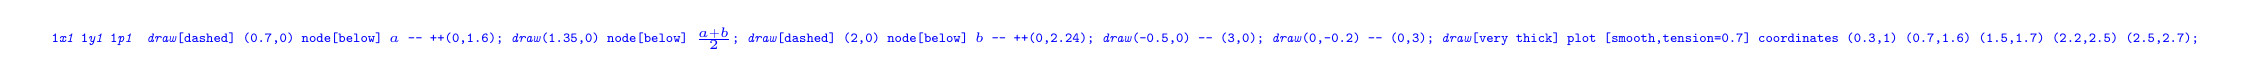
\begin{tikzpicture}

    \draw[dashed] (0.7,0) node[below] {$\vphantom{b}a$} -- ++(0,1.6);
    \draw (1.35,0) node[below] {$\frac{a+b}{2}$};
    \draw[dashed] (2,0) node[below] {$b$} -- ++(0,2.24);
    \draw (-0.5,0) -- (3,0);
    \draw (0,-0.2) -- (0,3);

    \draw[very thick] plot [smooth,tension=0.7]
    coordinates {(0.3,1) (0.7,1.6) (1.5,1.7) (2.2,2.5) (2.5,2.7)};
    \end{tikzpicture}


    \paragraph{Απλός κανόνας Simpson}
    \begin{align*}
    	P_2(x) &= f(a)l_0(x) +f\left(\frac{a+b}{2}\right)l_1(x)+f(b)
    	l_2(x) \\ &= f(a) \frac{(x-x_1)(x-x_2)}{(x_0-x_1)(x_0-x_2)}
    	+ f\left(\frac{a+b}{2}\right)
    	\frac{(x-x_0)(x-x_2)}{(x_1-x_0)(x_1-x_2)}
    	+ f(b) \frac{(x-x_0)(x-x_1)}{(x_2-x_0)(x_2-x_1)}
    	\\[3ex]
    	I_{\mathrm S} &= \int_a^b P_2(x)\dif x
    	\\ &= \dots = \frac{b-a}{6} \left[
    	f(a)+4f\left(\frac{a+b}{2}\right)+f(b) \right] \\[3ex]
    	E_{\mathrm S} &= I\left(f(x)\right)-I\left(P_2(x)\right) = \dots
    	\\ &= -\frac{\left(\frac{b-a}{2}\right)^5}{90} f^{(4)}(z) \\
    	\left|E_{\mathrm S}\right| &\leq
    	\frac{\left(\frac{b-a}{2}\right)^5}{90}\max_{a<z<b}\left\lvert f^{(4)}(z)\right\rvert
    \end{align*}

    \paragraph{Σύνθετος κανόνας Simpson}
    Το αρχικό διάστημα χωρίζεται σε \( 2N \) τμήματα:

    \begin{tikzpicture}[scale=.7,xscale=1.4]
    \draw (0,0) -- (0,-1) node[below] {$x_0$};
    \draw (0.5,0) -- ++(0,-0.7) node[below] {$x_1$};
    \draw (1,0) -- ++(0,-1) node[below] {$x_2$};
    \draw (1.5,0) -- ++(0,-0.7) node[below] {$x_3$};
    \draw (2,0) -- ++(0,-1) node[below] {$x_4$};
    \draw (2.5,0) -- ++(0,-0.7) node[below] {$x_5$};
    \draw (3,0) -- ++(0,-1) node[below] {$x_6$};
    \end{tikzpicture}

    Εφαρμόζουμε τον απλό κανόνα Simpson σε πολλά διαστήματα:
    \[
    a = x_0 \ < x_1 < x_2 < \cdots < x_{2N-1} < \ x_{2N} = b
    \]
    με απόσταση:
    \[
    h = \frac{b-a}{N} \qquad x_i = x_0 + i\frac{h}{2}
    \]
    και διαστήματα:
    \[
    \left[x_i,\ x_{i+2}\right], \qquad i=0,2,4,\dots,2N-2
    \]

    Οπότε τελικά έχουμε: \begin{align*}
    	I_{\mathrm S,2N} &= \frac{h}{6} \left[f(x_0)+4f(x_1)+f(x_2)
    	+f(x_2)+4f(x_3)+f(x_4)+\dots + f(x_{2N-2}) + 4f(x_{2N-1})
    	+f(x_{2N})\right] \\ &=
    	\frac{h}{6} \left[f(x_0)+4f(x_1)+2f(x_2)+4f(x_3)+2f(x_4)+\dots
    	+ 2f(x_{2N-2}) + 4f(x_{2N-1})+f(x_{2N})\right]
    \end{align*}

    Και για το σφάλμα, με αρκετές πράξεις προκύπτει:
    \begin{align*}
    	E{\mathrm S,2N} &= -n \frac{\left(\frac{h}{2}\right)^5}{90}
    	f^{(4)}(z),\quad a<z<b \\
    	&= -\frac{\left(\frac{h}{2}\right)^4}{180}(b-a)f^{(4)}(z) \\
    	\left|E_{\mathrm S,2N}\right| &\leq
    	\frac{\left(\frac{h}{2}\right)^4}{180}(b-a)
    	\max_{a<z<b} \left\lvert f^{(4)}(z)\right\rvert
    \end{align*}

    \subsection{Κανόνας Μέσου Σημείου}
    Ανοικτοί τύποι Newton-Cotes (μέχρι στιγμής έχουμε ασχοληθεί με
    κλειστούς τύπους Newton-Cotes).

    \paragraph{Απλός κανόνας μέσου σημείου}

    Η ιδέα είναι να παίρνουμε ένα παραλληλόγραμμο με ύψος όμως που να
    μην αντιστοιχεί στο άκρο του διαστήματος, αλλά στο μέσον του:

    \begin{center}
    	\begin{tikzpicture}[scale=1.7]
    	\filldraw[draw=gray,fill=green!80!blue!50!white] (0.8,0) rectangle (1.8,1.3);

    	\draw (-0.5,0) -- (2.3,0);
    	\draw (0,-0.5) -- (0,2.2);

    	\draw (0.8,0) node[below] {$a$} -- ++(0,0.85);
    	\draw[dashed] (0.8,0.85) -- (0,0.85) node[left] {$f(a)$};
    	\draw[dashed] (1.3,0) node[below] {$\frac{a+b}{2}$} -- ++(0,1.3) -- (0,1.3);
    	\draw[dashed] (1.3,1.3) -- (1.8,1.3);
    	\draw[dashed] (0.8,0.85) -- (1.8,0.85);
    	\draw (1.8,0) node[below] {$b$} -- ++(0,2);
    	\draw[dashed] (1.8,2) -- (0,2) node[left] {$f(b)$};

    	\draw[very thick,blue] plot [smooth,tension=1] coordinates {(-0.2,0.5) (1,1) (1.9,2.2)};

    	\end{tikzpicture}
    \end{center}

    \begin{align*}
    	I_{\mathrm M} &= (b-a)\cdot f\left(\frac{a+b}{2}\right) \\
    	E_{\mathrm M} &= \frac{(b-a)^3}{24}f''(z) \quad a<z<b
    \end{align*}

    \paragraph{Σύνθετος κανόνας μέσου σημείου}
    \begin{align*}
    	I_{\mathrm M, N} &= hf\left(x_0+\frac{h}{2}\right)
    	+hf\left(x_1+\frac{h}{2}\right)+\dots
    	+hf\left(x_{N-1}+\frac{h}{2}\right)
    	\\ &= h \sum_{i=0}^{N-1} f\left(x_i+\frac{h}{2}\right) \\
    	E_{\mathrm M, N} &= \frac{h^2}{24} (b-a) f''(z) \qquad a<z<b
    	\\ \left|E_{\mathrm M,N}\right| &\leq \frac{h^2}{24}(b-a)
    	\max_{a<z<b}\left|f''(z)\right|
    \end{align*}

    \subsection{Ασκήσεις}
    \paragraph{Άσκηση}
    Να υπολογιστεί το ολοκλήρωμα
    \[
    \mathlarger{I=\int_{0}^{1} \frac{1}{1+x}\dif x}
    \]
    με τον κανόνα του παραλληλογράμμου για \( N=1 \) και \( N=10 \)
    διαστήματα.

    \subparagraph{Λύση για \( N=1 \)}
    \begin{align*}
    	I_R &= f(0)\big(1-0\big) = 1\cdot 1 = 1 \\[3ex]
    	\left|E_R\right| &\leq \frac{(b-a)^2}{2}\max_{0<z<1}\left|
    	f(z)\right| \\ f'(z) &= \frac{1}{(1+z)^2} \\
    	\max_{0<z<1} \left|f'(z)\right| &= 1 \intertext{Άρα}
    	\left|E_R\right| &\leq \frac{(b-a)^2}{2}\max_{0<z<1}\left|
    	f(z)\right| = \frac{1}{2}\cdot 1 = \frac{1}{2}
    \end{align*}

    \subparagraph{Λύση για \( N=10 \)}
    \begin{align*}
    	I_{R,10} &= h\left(f(x_0)+f(x_1)+\dots+f(x_{N-1})\right) \\
    \end{align*}
    \[
    \begin{array}{r|c|c|c|c|c|c|c}
    x_k & 0 & 0.1 & 0.2 & 0.3 & \cdots & 0.9 & 1 \\ \hline
    f(x_k) & 1 & 0.9091 & 0.8333 & 0.7692 & \cdots & 0.5263 & 0.5
    \end{array}
    \]
    \begin{align*}
    	I_{R,10} &= 0.1\big(
    	1+0.9091+0.8333+0.7962+\dots+0.5263
    	\big) = 0.7188 \\ \left|E_{R,10}\right| &\leq \frac{h}{2}
    	(b-a) \max_{a<z<b}\left|f'(z)\right| = \frac{0.1}{2}\cdot
    	1\cdot 1 = 0.05
    \end{align*}

    \subparagraph{Λύση με κανόνα μέσου σημείου}
    \begin{align*}
    	I_M &= (b-a) \cdot f\left(\frac{a+b}{2}\right)
    	= 1 \cdot f\left(\frac{1}{2}\right) = 0.6667 \\
    	|E_M| &\leq \frac{(b-a)^3}{24} \max_{a<z<b} \left|f''(z)\right|
    	\intertext{\(
    		\max\limits_{0<z<1}\left|f''(z)\right|=
    		\max\limits_{0<z<1}\left|
    		\frac{2}{(1+x)^3}
    		\right| = 2\) για $x=0$}
    	&= \frac{1}{24}\cdot 2 = 0.0833
    \end{align*}

    \begin{tabular}{c|c|c}
    	Τύπος & Τιμή & Σφάλμα \\
    	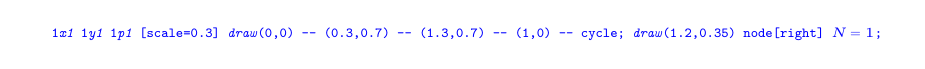
\begin{tikzpicture}[scale=0.3]
    	\draw (0,0) -- (0.3,0.7) -- (1.3,0.7) -- (1,0) -- cycle;
    	\draw (1.2,0.35) node[right] {$N=1$};
    	\end{tikzpicture}&  1 & 0.5  \\
    	\hline
    	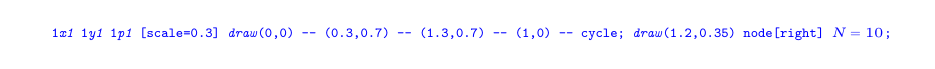
\begin{tikzpicture}[scale=0.3]
    	\draw (0,0) -- (0.3,0.7) -- (1.3,0.7) -- (1,0) -- cycle;
    	\draw (1.2,0.35) node[right] {$N=10$};
    	\end{tikzpicture}& 0.7188 & 0.05  \\
    	\hline
    	Μέσου Σημείου & 0.6667  & 0.0833 \\
    \end{tabular}

    \paragraph{Άσκηση}
    Να υπολογιστεί το ολοκλήρωμα
    \[
    I = \mathlarger{\int_{1}^{3}
    	\left(x+\frac{1}{x^2}\right)\dif x
    	}
    \]
    με τη μέθοδο τραπεζίου για \( N=6 \).
    \subparagraph{Λύση}
    \( 1=x_0<x_1<\dots<x_6=3 \)

    \begin{align*}
    I_{T,6} &= \frac{h}{2}\left[
    f(x_0)+2f(x_1)+2f(x_2)+2f(x_3)+2f(x_4)+2f(x_5)+f(x_6)
    \right]
    \end{align*}
    \(h=\frac{b-a}{N}=\frac{3-1}{6}=\frac{1}{3}\)

    \[
    \begin{array}{r|c|c|c|c|c|c|c}
    x_i & 1 & 1+\sfrac{1}{3} & 1+\sfrac{2}{3} & 2 & 2+\sfrac{1}{3}
    & 2+\sfrac{2}{3} & 3 \\ \hline
    f(x_i) & 2 & \sfrac{91}{48} & \sfrac{152}{75} & \sfrac{9}{4} &
    \sfrac{370}{147}  & \sfrac{532}{192} & \sfrac{28}{9}
    \end{array}
    \]

    Άρα:
    \begin{align*}
    	I_{T,6} &= \frac{1}{6} \left[
    	2+2\cdot\frac{91}{48}+2\cdot\frac{152}{75}+2\cdot\frac{9}{4}
    	+2\cdot\frac{370}{147}+2\cdot\frac{532}{192}+\frac{28}{9}
    	\right] = 4.684 \\
    	E_{T,6} &\leq \frac{h^2}{12}(b-a)\max_{a<z<b}\left|f''(z)\right|
    	= \frac{\left(\sfrac{1}{2} \right)^2}{12}\cdot(3-1)
    	\cdot\max_{1<z<3}\frac{6}{z^4} = \frac{1}{9} \simeq 0.1111
    \end{align*}

    \paragraph{Άσκηση}
    Για τη συνάρτηση \( f \) γνωρίζουμε τον παρακάτω πίνακα τιμών:
    \[
    \begin{array}{r|c|c|c|c|c|c|c}
    	       & x_0 & x_1 & x_2 & x_3 & x_4 & x_5 & x_6 \\[2ex]
    	   x_i &  1  &  2  &  3  &  4  &  5  &  6  &  7  \\ \hline
    	f(x_i) & -1  &  0  & 0.5 &  2  & 1.5 &  3  &  5
    \end{array}
    \]

    Ζητείται να βρεθεί το ολοκλήρωμα \( \displaystyle \int_1^7 f(x)
    \dif x \) με κανόνα Simpson.

    \subparagraph{Λύση}
    Για να εφαρμόσουμε κανόνα Simpson, το κάθε διάστημα πρέπει να
    καταλαμβάνει 3 σημεία (τα δύο άκρα και το μέσο).

    \begin{tikzpicture}[scale=2.5,every node/.style={scale=1},xscale=.9]

    \draw (0,0) node[above] {$x_0$} -- +(0,-0.15) -- ++(0.6,-0.15) --++(0,0.15);
    \draw (0.7,0) -- +(0,-0.15) -- ++(0.6,-0.15) --++(0,0.15);
    \draw (1.4,0) -- +(0,-0.15) -- ++(0.6,-0.15) --++(0,0.15) node[above] {$x_6$};

    \draw (0.65,0) node[above] {$x_2$};
    \draw (1.3,0) node[above] {$x_4$};

    \draw(0.3,0.1) node[above] {$x_1$};
    \draw(1.0,0.1) node[above] {$x_3$};
    \draw(1.7,0.1) node[above] {$x_5$};


    \end{tikzpicture}

    Επομένως:
    \begin{gather*}
    	N = 3 \\
    	h=\frac{7-1}{3}
    \end{gather*}

    Άρα έχουμε:
    \begin{align*}
    	I &= \frac{h}{6} \left[
    	f(x_0)+4f(x_1)+2f(x_2)+4f(x_3)+2f(x_4)+4f(x_5)+f(x_6)
    	\right] \\ &= \frac{1}{3} \left[
    	-1+4\cdot 0 + 2\cdot 0.5 + 4\cdot 2 + 2\cdot 1.5 + 4\cdot 3+5
    	\right] \\ &= 9.333
    \end{align*}

    \section{Υπολογισμός Ιδιοτιμών}
    Δομή της ενότητας:
    \begin{itemize}
    	\item Εισαγωγή
    	\item Μέθοδος Δύναμης
    	\item Μετασχηματισμοί Householder
    	\item Παραγοντοποίηση QR
    \end{itemize}

    \textbf{Το πρόβλημα που καλούμαστε να λύσουμε είναι:} Δεδομένου
    ενός πίνακα \( A \in \mathbb R^{n\times n} \), να υπολογιστούν οι
    ιδιοτιμές \( \lambda_i \in \mathbb R \), και τα αντίστοιχα
    ιδιοδιανύσματα \( x_i \in \mathbb R^n \), \underline{\( x_i\neq 0 \)}
    τα οποία ικανοποιούν:
    \[
    Ax_i = \lambda x_i \quad \text{για } i =1,2,\dots,n
    \]

    \subsection{Εισαγωγή}
    \[
    \boxed{Ax =
    	\underset{\substack{\downarrow\\\mathclap{\text{ιδιοτιμές}}}}{
    		\lambda}
    	\overset{\substack{\mathclap{\text{ιδιοδιανύσματα}}\\\uparrow}}{
    		x}\hspace{25pt}
    	}
    \]

    ή:
    \begin{align*}
    	(A-\lambda I)x &= 0 \\
    	\det(A-\lambda I) &= 0, \text{ δηλαδή } x \in N(A-\lambda I),
    	\text{ όπου } N \text{ ο μηδενοχώρος}
    \end{align*}

    Δηλαδή πρέπει να λύσουμε ένα σύστημα \( n \) εξισώσεων και αγνώστων.

    Ορίζουμε και το χαρακτηριστικό πολυώνυμο ως:
    \[
    P(\lambda) = \det(A-\lambda I)
    \]

    \paragraph{Παράδειγμα}
    \[
    A = \left[\begin{matrix}
    3&2\\3&-2
    \end{matrix}\right]
    \]

    Τότε:
    \begin{gather*}
    	|A-\lambda I| = \left|\begin{matrix}
    	3-\lambda & 2 \\ 3 & -2-\lambda
    	\end{matrix}\right| = \lambda^2 -\lambda-12 \\
    	\lambda^2-\lambda-12 = 0 \implies\begin{cases}
    	\lambda_1 &= 4 \\ \lambda_2&=-3
    	\end{cases}
    \end{gather*}

    Τα παραπάνω \( \lambda \) είναι οι ιδιοτιμές, και τα ιδιοδιανύσματα
    είναι, για \( \lambda_1 = 4 \):
    \begin{gather*}
    	(A-4I)x = 0 \iff \left[\begin{matrix}
    	-1&2\\3&-6
    	\end{matrix}\right]x = 0 \\ N(A-4I)= \left\lbrace
    	a\left[\begin{matrix}
    	2\\1
    	\end{matrix}\right]: a \in\mathbb R, a\neq 0
    	 \right\rbrace
    \end{gather*}

    Αντίστοιχα προκύπτει:
    \[
    N(A+3I) = \left\lbrace a\left[
    \begin{matrix}
    -1\\3
    \end{matrix}
    \right] : a \in\mathbb R, a\neq 0 \right\rbrace
    \]

    \paragraph{}
    Αν ο πίνακας είναι τριγωνικός, οι ιδιοτιμές είναι μόνο τα διαγώνια
    στοιχεία του:
    \[
    \lambda_i = a_{ii}
    \]

    \begin{defn}{Φάσμα}{}
    	Το σύνολο όλων των ιδιοτιμών ενός πίνακα \( A \) ονομάζεται
    	\textbf{ΦΑΣΜΑ} του \( A \):
    	\[
    	\sigma(a)
    	\]
    \end{defn}

    \begin{defn}{Φασματική ακτίνα}{}
    	Το μέγιστο κατ' απόλυτη τιμή στοιχείο του φάσματος ονομάζεται
    	\textbf{φασματική ακτίνα} του \( A \) και συμβολίζεται:
    	\[
    	P(A) = \max\left\lbrace |\lambda|:\lambda \in \sigma(A)
    	\right\rbrace
    	\]

    	Δηλαδή είναι η μέγιστη κατ' απόλυτη τιμή ιδιοτιμή του \( A \).
    \end{defn}

    Επειδή ο υπολογισμός ορίζουσας είναι δύσκολη υπολογιστική διαδικασία,
    θα βρούμε αριθμητικούς τρόπους να τις βρίσκουμε/προσεγγίζουμε.

    \subsubsection{Άνω Φράγματα}
    \begin{defn}{}{}
    	Ορίζουμε:
    	\begin{align*}
    	r_i(A) &= \sum_{j=1}^{n} \left|a_{ij}\right|, \ \forall i\\
    	c_j(A) &= \sum_{i=1}^{n} \left|a_{ij}\right|, \ \forall j
    	\intertext{(τα αθροίσματα των απόλυτων τιμών των στοιχείων
    		κάθε γραμμής \& στήλης)}
    	r(A) &= \max\left\lbrace r_i(A): \forall i \right\rbrace\\
    	c(A) &= \max\left\lbrace c_j(A): \forall j \right\rbrace
    	\intertext{(το μέγιστο άθροισμα)}
    	\end{align*}
    \end{defn}

    \begin{theorem}{Gerschgorin}{}
    	Για πίνακα \( A \in \mathbb R^{n\times n} \), έστω ότι, για
    	κάθε γραμμή:
    	\[
    	R_i = r_i(A) - \left|a_{ii}\right| \ \forall i
    	\]
    	και έστω δίσκος \( C_i \) με ακτίνα \( R_i \) και κέντρο
    	\( a_{ii} \) (\( a_{ii}\in\mathbb C \)).

    	Τότε για κάθε \( \lambda \in \sigma(A) \) υπάρχει \( i \) όπου
    	\( \lambda \in C_i \), δηλαδή:
    	\[
    	\left|\lambda - a_{ii}\right| \leq R_i
    	\]
    \end{theorem}

    \paragraph{Συνέπεια}
    Έστω:
    \begin{align*}
    	\lambda &\in \sigma(A) \text{ ενός } A \in \mathbb R^{n\times n}
    	\\
    	\lvert\lambda\rvert &\leq r(A) \\[3ex]
    	\left|\lambda - a_{kk}\right| &\leq R_k \\
    	\left|(\lambda - a_{kk})+a_{kk}\right| &\leq
    	\left|\lambda - a_{kk}\right|+\left|a_{kk}\right|
    	\leq R_k + \left|a_{kk}\right| = r_k(A) \leq r(A)
    \end{align*}

    Επειδή \( r(A^{\mathrm T}) = c(A) \), ισχύει ότι:
    \[
    |\lambda| \leq \min\left\lbrace r(A),c(A) \right\rbrace
    \]

    Επομένως για το προηγούμενο παράδειγμα:
    \begin{align*}
    A&=\left[\begin{matrix}
    3&2\\3&-2
    \end{matrix}\right]
    \\ \left.\begin{array}{rr}
    r_1(A) &= 5 \\ r_2(A) &= 5
    \end{array}\right\rbrace r(A) &= 5 \\
    \left.\begin{array}{rr}
    c_1(A) &= 6 \\ c_2(A) &= 4
    \end{array}\right\rbrace c(A) &= 6 \\
    |\lambda| &\leq \min\left\lbrace 5,6 \right\rbrace = 5
    \end{align*}

    \subsection{Μέθοδος δύναμης}
    Έχουμε έναν πίνακα \( A \) και κατατάσσουμε τις ιδιοτιμές του:
    \[
    \left|\lambda_1\right| \geq \left|\lambda_2\right|
    \geq \dots \geq \left|\lambda_n\right|
    \]
    με ιδιοδιανύσματα:
    \[
    x_1,x_2,\dots,x_n
    \]
    που γνωρίζουμε από τη θεωρία γραμμικής άλγεβρας ότι είναι γραμμικά
    ανεξάρτητα, επομένως σχηματίζουν μία βάση, με ένα τυχαίο διάνυσμα:
    \begin{align*}
    v_0 &= a_1x_1+a_2x_2+\dots+a_nx_n
    \intertext{πολλαπλασιάζουμε με \( A \):}
    Av_0 &= a_1Ax_1+a_2Ax_2+\dots + a_nAx_n \\
         &= a_1\lambda_1 x_1+a_2\lambda_2 x_2 +\dots + a_n\lambda_n
         x_n \\
    A^2v_0 &= a_1\lambda_1^2 x_1 +a_2\lambda_2^2 x_2+\dots +
    a_n\lambda_n^2x_n \\
    &\vdots \\
    \underbrace{A^kv_0}_{v_k} &= a_1\lambda_1^k
    x_1+a_2\lambda_2^kx_2+\dots +
    a_n\lambda_n^k x_n \\
    \frac{1}{\lambda_1^k} v_k &=
    a_1x_1 + a_2\left(\frac{\lambda_2}{\lambda_1}\right)^k
    x_2+\dots + a_n\left(\frac{\lambda_n}{\lambda_1}\right)^k x_n \\
    \lim_{k\to \infty} \frac{1}{\lambda_1^k} v_k &= a_1x_1
    \end{align*}
    Επειδή \( k\to \infty \) και μπορεί να εμφανιστούν πολύ μεγάλοι ή
    πολύ μικροί αριθμοί, θα κανονικοποιήσω το \( v_k \).

    \subsubsection{Αλγόριθμος}
    \textbf{Είσοδος:} \( A \in \mathbb R^{n\times n},
    u_0 \in \mathbb R^n \):

    \begin{algorithm}[H]
    	\For{k=0,1,\dots}{
            \( v_{k+1} := A u_k \)\;
            \( u_{k+1} := \frac{1}{\left\Vert v_{k+1}\right\Vert_\infty}
            v_{k+1} \)\;
            \If{\( \left\Vert u_{k+1}-u_k \right\Vert_\infty <
            	\epsilon \)}{go to 6}
    	}
\end{algorithm}

\paragraph{Παράδειγμα}
\begin{alignat*}{4}
A&=\begin{bmatrix}
2&1\\1&2
\end{bmatrix},\quad u_0=\left[\begin{matrix}
2\\1
\end{matrix}\right] \\
v_1 &= Au_0 = \left[\begin{matrix}
5\\4
\end{matrix}\right] && \implies u_1 && = \frac{1}{5}v_1 && = \left[
\begin{matrix}
1.0\\0.8
\end{matrix}\right] \\
v_2 &= Au_1 = \left[\begin{matrix}
2.8\\2.6
\end{matrix}\right] && \implies u_2 && = \frac{1}{2.8}v_2 && = \left[\begin{matrix}
1.0\\0.93
\end{matrix}\right] \\
v_3 &= Au_2 = \left[\begin{matrix}
2.92\\2.85
\end{matrix}\right] && \implies u_3 && = \frac{1}{2.92} v_3 && = \left[\begin{matrix}
1.0\\0.98
\end{matrix}\right] \\
v_4 &= Au_3 = \left[\begin{matrix}
2.98\\2.95
\end{matrix}\right]
\end{alignat*}

\subsection{Μετασχηματισμοί Householder}
Από τη γραμμική άλγεβρα γνωρίζουμε ότι οι όμοιοι πίνακες έχουν ίδιες
ιδιοτιμές:
\begin{gather*}
	A,B \in \mathbb R^{n\times n} \\
	\boxed{B = S^{-1}AS}
\end{gather*}

Αν για τον \( A \) έχω υπολογίσει την \( \lambda_1 \), θα είναι χρήσιμο
να μπορώ να βρω έναν πίνακα:
\[
HAH^{-1} = \left[ \begin{array}{c|ccccc}
\lambda_1 & x & x & x & \dots & x \\ \hline
0 & & & & & \\
0 & & & A_1 & & \\
\vdots & & & & & \\
0 & & & & &
\end{array} \right]
\]

\begin{align*}
	\det(A-\lambda I) \overset{\text{όμοιοι}}{=}
	\det(HAH^{-1}-\lambda I) =
	(\lambda_1-\lambda)\det(A_1 - \lambda I)
\end{align*}

Αν \( e_1=\left[\begin{matrix}
1\\0\\ \vdots \\ 0
\end{matrix}\right] \)
\begin{align*}
	HAH^{-1} e_1 &= \lambda_1 e_1 \\
	A(H^{-1}e_1) &= \lambda_1 (H^{-1}e_1)
\end{align*}
Δηλαδή ψάχνω \( H \) ώστε:
\begin{align*}
	H^{-1}e_1 &= x_1 \\
	\Aboxed{Hx_1 &= e_1}
\end{align*}
κάτι που θα μου δώσει ο Householder.

\subsection{Παραγοντοποίηση QR (Εισαγωγή)}
Μετατρέπω έναν πίνακα \( A \) σε γινόμενο 2 πινάκων \( Q \) και
\( R \), όπου ο \( Q \) ορθογώνιος και ο \( R \) άνω τριγωνικός:
\[
A =
\underset{\substack{\downarrow\\\mathclap{\text{ορθογώνιος}}}}{Q}
\cdot
\overset{\substack{\mathclap{\text{άνω τριγωνικός}}\\\uparrow}}{R}
\]

Για κάποιες επαναλήψεις:
\[
A_0 = A
\]
\[
\begin{cases}
A_0 = Q_1R_1, &\quad \text{θέτω } A_1 = R_1Q_1 \\
A_1 = Q_2R_2, &\quad \text{θέτω } A_2 = R_2Q_2 \\
\quad \vdots &\quad \quad \vdots \\
A_{k-1} = Q_kR_k, &\quad \text{θέτω } A_k = R_kQ_k \\
\end{cases}
\]

Η μέθοδος αυτή συγκλίνει σε έναν ημιτριγωνικό πίνακα (τον
\( A_k \)). Από τον \( A_0 \) ξεκινώ, τον παραγοντοποιώ σε
\( Q_1R_1 \) και βρίσκω τον \( A_1 = R_1Q_1 \). Παραγοντοποιώ τον
\( A_1 \) σε γινόμενο \( QR \) κ.ό.κ.

\textbf{Για έναν ημιτριγωνικό πίνακα:}
\[ \left[
\begin{matrix}
\circ & & & & \\
& \circ & & & \\
& & \Box & & \\
& & & \Box & \\
& & & & \ddots
\end{matrix} \right]
\]

Ο πίνακας αυτός είναι άνω τριγωνικός, απλά σε κάποιες θέσεις στη
διαγώνιο έχει \( 2\times 2 \) πίνακες.

\paragraph{Παράδειγμα}
Να βρεθούν οι ιδιοτιμές του πίνακα \( A \) με παραγοντοποίηση
\( QR \):
\[
A = \left[\begin{matrix}
1&2&3 \\ 0 & 1 & 5 \\ 0 & -3 & 2
\end{matrix}\right]
\]
\subparagraph{Λύση}
Ο \( A \) είναι ήδη ημιτριγωνικός (ουσιαστικά είναι ο \( A_k \)):
\[
A = \left[\begin{matrix}
1 & \\ 0 & \boxed{B}
\end{matrix}
\right] \quad \text{όπου } B = \left[
\begin{matrix}
1 & 5 \\ -3 & 2
\end{matrix}\right]
\]

Η μία ιδιοτιμή είναι το \( \lambda_1 = 1 \).

Οι μιγαδικές ιδιοτιμές θα προκύψουν από τον πίνακα \( B \):
\begin{align*}
	\det(B-\lambda I) = 0 \implies
	\left|\begin{matrix}
	1-\lambda & 5 \\ -3 & 2-\lambda
	\end{matrix}
	\right| = 0 \implies \lambda^2 -3\lambda + 17 = 0
	\implies \lambda_{2,3} =\frac{3}{2} \pm i\frac{\sqrt{59}}{2}
\end{align*}

\paragraph{Παράδειγμα}
Να βρεθούν οι ιδιοτιμές του \( A \) με τη μέθοδο παραγοντοποίησης
\( QR \):
\[
A = \left[\begin{matrix}
6&-1& 5 \\ -3 & 2 & -1 \\ 2 & 4 & 2
\end{matrix}
\right]
\]
\subparagraph{Λύση}
Σύμφωνα με τη μέθοδο:
\begin{gather*}
	A = A_0 \\
	A_0 = Q_1R_1 = \left[\begin{matrix}
	0.85&-0.11&0.50\\
	-0.42&0.38&0.81\\
	0.28&0.91&-0.28
	\end{matrix}\right] \cdot \left[\begin{matrix}
	7&-0.57&5.28\\
	0&4.54&6.88\\
	0&0&1.13
	\end{matrix}
	\right]
	\intertext{(Θα δούμε αργότερα πώς βρίσκουμε τους \( Q_1R_1 \))}
	A_1=R_1Q_1 = \left[\begin{matrix}
	7.75&5.83&1.55\\-1.69&2.56&3.46\\0.32&1.03&-0.31
	\end{matrix}\right]
\end{gather*}

Τώρα παραγοντοποιώ τον \( A_1 \) σε γινόμενο QR:
\[
A_1 = Q_2R_2 \implies A_2 = R_2Q_2
\]

Μετά από 6 επαναλήψεις προκύπτει:
\[
A_6 = \left[\begin{matrix}
6.06 & 5.30 & 1.05 \\
-0.17 & 5.07 & -2.63 \\
0 & 0 & -1.13
\end{matrix}\right]
\]

Ο πίνακας \( A_6 \) είναι ημιτριγωνικός. Στην διαγώνιο βρίσκουμε
ότι \( \lambda_3 = -1.13 \). Ύστερα μέσω του \( B = \left[
\begin{matrix}
6.06&5.30 \\ -0.17&5.07
\end{matrix}
\right] \)
θα βρω τις
\( \lambda_{1,2} \):
\[
\det(B-\lambda I) = 0 \implies \lambda_{1,2} = 5.57
\pm i0.81
\]

\subsection{Παραγοντοποίηση QR}
\paragraph{Το πρόβλημα}
Δεδομένου ενός πίνακα \( A \), να βρεθούν 2 πίνακες
\( Q \) (ορθογώνιος), \( R \) (άνω τριγωνικός), έτσι ώστε:
\[
\mathlarger{A = Q \cdot R}
\]

\subsubsection{Εισαγωγή}
Ένα σύνολο διανυσμάτων \( \left\lbrace x_1,x_2,\dots,
x_n \right\rbrace \) του χώρου \( V \) λέγονται ορθογώνια αν ανά
2 μεταξύ τους είναι κάθετα:
\[
(x_i,x_j) = 0 \quad \forall i \neq j
\]

Τα διανύσματα \( x_1,x_2,\dots, x_n \) λοιπόν είναι μεταξύ τους
γραμμικά ανεξάρτητα. Εάν σε αυτά τα διανύσματα προσθέσω (εκτός
της ορθογωνιότητας) την ιδιότητα της
\textbf{μοναδιαίας νόρμας/μήκους/μέτρου}, ονομάζω τα \( x_1,x_2,
\dots, x_n \) \textbf{ορθοκανονικά}. Τότε ισχύει και η παρακάτω
ιδιότητα:

\paragraph{Kroenecker Delta}

Όταν έχω μία σχέση μεταξύ δύο αντικειμένων:
\begin{align*}
	(x_i,x_j) &= 0 \quad \text{για } i \neq j \\
	          &= 1 \quad \text{για } i = j
\end{align*}
αυτή αναπαριστά το δέλτα του Kroenecker:
\[
(x_i,x_j) = \delta_{ij}
\]

Για να μετατρέψω το ορθογώνιο σύστημα σε ορθοκανονικό, αρκεί
να πάρω κάθε διάνυσμα βάσης, και να το "μειώσω" ώστε να έχει
μέτρο τη μονάδα (\textbf{κανονικοποίηση}):
\[
x_i := \frac{x_i}{\Vert x_i \Vert}
\]

Για παράδειγμα, αν \( x_i=\left[\begin{matrix}
x_1\\x_2\\x_3
\end{matrix}\right] \), τότε:
\begin{align*}
	\Vert x_i \Vert^2 &= x_1^2+x_2^2+x_3^2 \\
	\Vert x_i \Vert &= \sqrt{x_1^2+x_2^2+x_3^2} \\
	x_i &= \left[
	\begin{matrix}
	\frac{x_1}{\sqrt{x_1^2+x_2^2+x_3^2}} \\
	\frac{x_2}{\sqrt{x_1^2+x_2^2+x_3^2}} \\
	\frac{x_3}{\sqrt{x_1^2+x_2^2+x_3^2}}
	\end{matrix}
	\right]
\end{align*}

\paragraph{}
Ας υποθέσουμε ότι έχουμε \( n \) ορθοκανονικά διανύσματα βάσης
σε έναν χώρο διάστασης \( n \):
\[
\left\lbrace x_1,x_2,\dots,x_n \right\rbrace
\]

Επομένως κάθε διάνυσμα \( X \) του χώρου γράφεται σαν γραμμικός
συνδυασμός των διανυσμάτων βάσης:
\[
X = \sum_{i=1}^{n} c_i x_i
\]
και επειδή η βάση είναι ορθοκανονική, αποδεικνύεται ότι οι
συντελεστές \( c_i \) προκύπτουν από το εσωτερικό γινόμενο:
\[
c_i = (x_i,X)
\]

\textit{Πράγματι:}
\begin{align*}
	\left(x_i,X\right) &= \left(
	x_i, \sum_{j=1}^{n} c_j x_j \right)
	\intertext{Από ιδιότητα του εσωτερικού γινομένου
		\( (ax+by,z)=a(x,y)+b(y,z) \)}
	&= \sum_{j=1}^{n} c_j(x_i,x_j)
	\\ &= \sum_{j=1}^{n} c_i \cdot \delta_{ij} = c_i.
\end{align*}

\subsubsection{Ορθογώνιος πίνακας}
Έστω ότι στον χώρο \( \mathbb R^n \) έχουμε \( n \) ορθοκανονικά
διανύσματα \( q_1,q_2,\dots,q_n \).

Τον πίνακα που φτιάχνουμε με αυτά τα διανύσματα:
\[
Q = \left[\begin{matrix}
& & & \\ q_1 & q_2 & \dots & q_n \\ & & &
\end{matrix}\right]
\]
τον ονομάζουμε \textbf{ορθογώνιο} πίνακα.

Για αυτόν προκύπτει αν δούμε τις πράξεις:
\[
\boxed{Q^{\mathrm T}Q = I},
\]
δηλαδή ο \textit{ανάστροφός του} είναι ο \textit{αντίστροφός} του:
\[
Q^{-1} = Q^{\mathrm T}
\]

\paragraph{Εσωτερικά γινόμενα}
Θα δείξουμε ότι το εσωτερικό γινόμενο δύο διανυσμάτων \( x,y \) ενός χώρου
δεν αλλάζει αν τα πολλαπλασιάσουμε με τον \( Q \), δηλαδή
\( \mathlarger{(Qx,Qy) = (x,y)} \):
\begin{align*}
	(Qx,Qy) &= (Qx)^{\mathrm T}Qy \\
	&= x^{\mathrm T} \underbrace{Q^{\mathrm T}Q}_{I} y\\
	&= x^T \, y = (x,y).
\end{align*}

Επομένως, παρατηρώ ότι:
\[
\left\Vert Qx \right\Vert^2
= (Qx,Qx) = (x,x) = \left\Vert x \right\Vert^2
\]

\paragraph{Συγκεντρωτικά οι ιδιότητες του \( Q \in \mathbb
	 R^{n\times n} \)}
\begin{enumerate}
	\item Στήλες \( Q \) είναι μια ορθοκανονική βάση του
	\( \mathbb R  \)
	\item \( Q^{\mathrm T} Q = I \)
	\item \( Q^{-1} = Q^{\mathrm T} \)
	\item \( (Qx,Qy) = (x,y) \)
	\item \( \left\Vert Qx \right\Vert = \Vert x\Vert \)
\end{enumerate}

\subsection{Μετασχηματισμοί Householder}
Ο μετασχηματισμός Householder είναι ένας πίνακας που μετασχηματίζει
ένα διάνυσμα, ώστε π.χ. να έχει ίδια κατεύθυνση αλλά διαφορετικό
μέτρο.

\paragraph{Το πρόβλημα}
Δεδομένου ενός διανύσματος \( x \in \mathbb R^n \) και σταθεράς
\( k \in \left\lbrace 1,2,\dots,n \right\rbrace \), να βρεθεί ένας
\underline{πίνακας} \( H \), τέτοιος ώστε οι τελευταίες \( n-k \)
συνιστώσες του διανύσματος \( Hx \) να είναι μηδέν.

Δηλαδή οι τιμές του \( Hx \), κάτω από μία θέση που θέλω εγώ, να
είναι μηδενικές.

Αυτό το πρόβλημα θα λύσουν οι μετασχηματισμοί Householder:
\begin{defn}{}{}
Για κάποιο διάνυσμα \( u \in \mathbb R^n \) με
\underline{μοναδιαίο} μήκος (\( \Vert u\Vert_2 = 1 \)), ο πίνακας
\[
\boxed{H = I - 2uu^{\mathrm T}}
\]
ονομάζεται \textbf{μετασχηματισμός Householder}.
\end{defn}

Παρατηρούμε ότι (και προκύπτει με πράξεις), ότι ο \( H \) είναι
\textbf{συμμετρικός}.

Θα αποδείξουμε ότι ο \( H \) είναι \textbf{ορθογώνιος}!
\begin{align*}
	HH^{\mathrm T} &=
	(I-2uu^{\mathrm T})(I-2uu^{\mathrm T})^T \\
	&= (I-2uu^{\mathrm T})(I-2uu^{\mathrm T}) \\
	&= I-4uu^{\mathrm T} +
	\underbrace{4u\underbrace{u^{\mathrm T} u}_1
	u^{\mathrm T}uu^{\mathrm T}}_1 \\
	&= I
\end{align*}

\paragraph{}
Έχω:
\begin{gather*}
	Hx =y \text{ όπου για τον $y$, από την $k+1$ θέση και κάτω,
		μηδενικά} \\
	Hx = (I-2uu^{\mathrm T}) x = x-2uu^{\mathrm T}x=x-2(u^{\mathrm T}x)u
\end{gather*}

Όμως, το \( u^{\mathrm T}x \) είναι η προβολή του \( x \) στο \( u \).
Όπως ξέρω, η προβολή του διανύσματος \( \vec b \) πάνω στο διάνυσμα
\( \vec a \) γράφεται:
\[
\vec \rho = \frac{a^{\mathrm T}b}{a^{\mathrm T} a}\vec a
\]
Άρα για εμάς:
\[
\vec \rho = \frac{u^{\mathrm T}x}{\cancelto{1 \text{ αφού μοναδιαίο}}{
		u^{\mathrm T}u}} = (u^{\mathrm T}x)u
\]

Για να βρω τον \( Η \) ψάχνω το \( u \) στη σχέση
\( I-2uu^{\mathrm T} \).

Ορίζω το διάνυσμα \( y \) με την ίδια νόρμα (ευκλείδια) με το \( x \):
\[
\Vert x \Vert_2 = \Vert y \Vert_2
\]

Έτσι, ορίζω ακόμα το μοναδιαίο (κανονικοποιημένο) διάνυσμα \( u \) ως:
\[
u = \frac{x-y}{\Vert x-y \Vert}
\]

Θα δείξω ότι αυτό το \( u \) είναι μια πάρα πολύ καλή επιλογή:
\[
(I-2uu^{\mathrm T})x = y
\]
\subparagraph{Θέλω}
\[
x=\left[\begin{matrix}
x_1\\x_2\\ \vdots \\ x_k \\ \vdots \\ x_n
\end{matrix}\right]
\rightarrow
y=\left[\begin{matrix}
x_1 \\ x_2 \\ \vdots \\ x_{k-1}
\\ \pm \sqrt{x_k^2+x_{k+1}^2+\dots + x_n^2} \\
0 \\ 0 \\ \vdots \\ 0
\end{matrix}\right] \quad \text{(από το $k+1$ και κάτω, 0)}
\]

Αυτό γίνεται με το:
\[
u = \frac{x-y}{\Vert x-y \Vert}
\]

Θα βρω ακριβώς το \( u \):
\begin{gather*}
	(x-y) = \left[\begin{matrix}
	0 \\ 0 \\ \vdots \\ \mathsmaller{x_k -
	 \left(-\sgn(x_k)\cdot\sqrt{x_k^2+x_{k+1}^2+\dots + x_n^2} \right)
	}
	 \\ x_{k+1} \\ \vdots \\ \vdots \\ x_n
	 \end{matrix}
	\right]
\end{gather*}
Για ευκολία θέτω: \begin{equation}
\label{s_formula}
		\boxed{s=\sqrt{x_k^2+x_{k+1}^2+\dots + x_n^2}
			}\end{equation}
\begin{align}
\label{xy_formula}
	\Vert x-y \Vert &= \sqrt{
		\left(x_k+\sgn(x_k)s\right)+x_{k+1}^2+\dots + x_n^2
		} \nonumber \\ &= \sqrt{2s\left(s+|x_k|\right)}
\end{align}

Τελικά: \[
	\label{u_matrix}
	u = \frac{1}{\sqrt{2s\left(s+|x_k|\right)}} \left[
	\begin{matrix}
	0 \\ 0 \\ \vdots \\ \mathsmaller{x_k -
		\left(-\sgn(x_k)\cdot\sqrt{x_k^2+\dots + x_n^2} \right)
	}
	\\ x_{k+1} \\ \vdots \\ \vdots \\ x_n
	\end{matrix}
	\right]
\]

\paragraph{Παράδειγμα}
Επιθυμώ το παρακάτω \( x \) να έχει μηδέν στην 3\textsuperscript{η}
συνιστώσα: \[
x = \left[\begin{matrix}
7\\4\\3
\end{matrix}\right]
\]
\subparagraph{Επίλυση}
Είναι \( k=2 \). Θα χρησιμοποιήσω τις \eqref{s_formula} και \eqref{xy_formula}:
\begin{gather*}
	s = \sqrt{x_2^2+x_3^2} = \sqrt{4^2+3^2} = 5\\
	\Vert u \Vert = \Vert x-y \Vert = \sqrt{2\cdot 5
		\left(s+|x_k|\right)}= \sqrt{10(5+4)} = \sqrt{90}
	\intertext{$\sgn(x_k) = {\color{green} +}$}
	u = \frac{1}{\sqrt{90}} \left[\begin{matrix}
	0\\4 + {\color{green} + } 5 \\3
	\end{matrix}\right] = \frac{1}{\sqrt{90}} \left[\begin{matrix}
	0\\9\\3
	\end{matrix}\right]
\end{gather*}

Άρα:
\begin{align*}
	H &= I-2uu^{\mathrm T} = I - \frac{2}{90}\left[\begin{matrix}
	0\\9\\3
	\end{matrix}\right]\left[\begin{matrix}
	0&9&3
	\end{matrix}\right] = I-\frac{2}{90}\left[\begin{matrix}
	0&0&0\\0&81&27\\0&27&9
	\end{matrix}\right] \\ &= \left[\begin{matrix}
	1&0&0\\0&1&0\\0&0&1
	\end{matrix}\right] - \frac{2}{90}\left[\begin{matrix}
	0&0&0\\0&81&27\\0&27&9
	\end{matrix}\right] = \frac{1}{5}\left[\begin{matrix}
	5&0&0\\0&-4&-3\\0&-3&4
	\end{matrix}\right] \\
	H\cdot x &= \dots = \left[\begin{matrix}
	7\\-5\\0
	\end{matrix}\right] \quad \text{(επαλήθευση)}
\end{align*}

\paragraph{}
Για να γράψω έναν πίνακα \( A \) με μορφή:
\[
A = Q \cdot R
\]
λειτουργώ ως εξής:
\begin{gather*}
	H_1 \cdot A = \left[\begin{matrix}
	H_1a_1 & H_1a_2 & \dots & H_1 a_n
	\end{matrix}\right] = \left[\begin{matrix}
	* & * & * & \hdots & * \\
	0 & * & * & \hdots & * \\
	0 & * & * & \hdots & * \\
	\vdots & \vdots & \vdots & \ddots & \vdots \\
	0 & * & * & \hdots & *
	\end{matrix}\right] = A_1.
	\intertext{Βρίσκω τον $A_1$, από αυτόν υπολογίζω τον $H_2$, και
		ύστερα βρίσκω το γινόμενο $H_2\cdot A_1$}
	H_2 \cdot A_1 = \left[\begin{matrix}
	* & * & * & * & \hdots & * \\
	0 & * & * & * & \hdots & * \\
	0 & 0 & * & * & \hdots & * \\
	0 & 0 & * & * & \hdots & * \\
	\vdots & & \vdots & \vdots & \ddots & \vdots \\
	0 & 0 & * & * & \hdots & *
	\end{matrix}\right] = A_2 \\
	H_{n-1}A_{n-2} = \left[\begin{matrix}
	* & * & * & * & \hdots & * \\
	0 & * & * & * & \hdots & * \\
	0 & 0 & * & * & \hdots & * \\
	0 & 0 & 0 & * & \hdots & * \\
	\vdots & & \vdots & \vdots & \ddots & \vdots \\
	0 & 0 & 0 & 0 & \hdots & *
	\end{matrix}\right] = A_{n-1} = R
\end{gather*}

Τελικά δηλαδή:
\[
\boxed{H_{n-1}H_{n-2}\cdots H_1\, A = R}
\]

\[
H \begin{matrix}
\nearrow \text{ \small συμμετρικός} \\ \searrow \text{\small ορθογώνιος}
\end{matrix}
\]\[
H^{\mathrm T} = H^{-1}
\]\begin{align*}
	A &= H_1^{\mathrm T} H_2^{\mathrm T}\dots
	H_{n-1}^{\mathrm T}R \\
	A &= \underbrace{H_1H_2\dots H_{n-1}}_QR
	\intertext{Δηλαδή φτάνουμε στο πολυπόθητο:}
	\Aboxed{A &= QR} \\
	\underset{m\times n}{A} &= \underset{m\times m}{Q} \times
	\underset{m\times n}{\vphantom{Q}R} \rightarrow
	\left[\begin{matrix}
	n\times n \text{ άνω τριγωνικός }  \\ \hline
	\underset{\text{$m\times n$ γραμμές}}{0}
	\end{matrix}\right]
\end{align*}

\paragraph{Άσκηση}
Δίνεται ο πίνακας \( \mathlarger{X=\left[\begin{matrix}
	-3\\4\\12 \end{matrix}
	\right]} \). Να βρεθεί πίνακας \( H \) ώστε ο \( Hx \) να έχει μηδέν
τις τελευταίες 2 συνιστώσες.
\subparagraph{Λύση}
\begin{gather*}
	k=1 \\ s=\sqrt{x_1^2+x_2^2+x_3^2} = \sqrt{(-3)^2+4^2+12^2} = 13
	\\ u = \frac{1}{\sqrt{2\cdot 13\cdot (13+3)}}\left[
	\begin{matrix}
	x_1+\mathrm{sgn}(x_1)\cdot s\\ x_2 \\ x_3
	\end{matrix}\right] \overset{\cdots}{=} \frac{1}{\sqrt{26}} \left[
	\begin{matrix}
	-4\\1\\3
	\end{matrix}\right] \\
	H = I-2uu^{\mathrm T} = \left[\begin{matrix}
	1&0&0\\0&1&0\\0&0&1
	\end{matrix}\right] - 2\frac{1}{\sqrt{26}}\left[\begin{matrix}
	-4\\1\\3
	\end{matrix}\right]\frac{1}{\sqrt{26}}\left[\begin{matrix}
	-4&1&3
	\end{matrix}\right]
	= \frac{1}{13}\left[\begin{matrix}
	-3&4&12\\4&12&-3\\12&-3&4
	\end{matrix}\right]
\end{gather*}
Όντως, για επαλήθευση παρατηρούμε ότι:
\[
Hx = \left[\begin{matrix}
13\\0\\0
\end{matrix}\right]
\]

\paragraph{Άσκηση}
Να παραγοντοποιηθεί/γραφεί σε μορφή \( QR \) ο πίνακας \( A =
\left[\begin{matrix}
1&5&6\\2&-4&-5\\2&3&17
\end{matrix}\right] \).
\subparagraph{Λύση}
Στην πρώτη στήλη:
\begin{gather*}
	a_1 = \left[\begin{matrix}
	1\\2\\2
	\end{matrix}\right] \qquad k=1 \\
	s=\sqrt{1^2+2^2+2^2}=3 \\
	u_1 = \frac{1}{\sqrt{2s(s+|x_1|)}}\left[\begin{matrix}
	x_1+s\\x_2\\x_3
	\end{matrix}\right] = \frac{1}{\sqrt{24}}\left[\begin{matrix}
	4\\2\\2
	\end{matrix}\right] \\
	H_1 = I-2u_1u_1^{\mathrm T} \overset{\cdots}{=}
	\frac{1}{3}\left[\begin{matrix}
	-1&-2&-2\\-2&2&-1\\-2&-1&2
	\end{matrix}\right] = Q \\
	H_1A = \left[\begin{matrix}
	-3&-1&-10\\0&-7&-13\\0&0&9
	\end{matrix}\right] = R
\end{gather*}

\paragraph{Άσκηση}
Να βρεθεί η παραγοντοποίηση QR του πίνακα \( A \):
\[
A = \left[\begin{matrix}
+1&+2&3\\+2&9&2\\+2&2&1
\end{matrix}\right]
\]
\subparagraph{Λύση}
\begin{itemize}
	\item Για \( k=1 \) Householder:
	\begin{gather*}
		Q_1 = \left[\begin{matrix}
		1\\2\\2
		\end{matrix}\right] \\
		H_1 = \frac{1}{3} \left[\begin{matrix}
		-1&-2&-2\\-2&2&-1\\2&-1&2
		\end{matrix}\right] \\
		A_1 = H_1A = \left[\begin{matrix}
		-3 & -8 & -3 \\ 0 &4 & -1 \\ 0 & -3 & -2
		\end{matrix}\right]
	\end{gather*}
	\item Για \( k=2 \) Householder:
	\begin{gather*}
		Q_2' = \left[\begin{matrix}
		-8 \\ 4 \\ -3
		\end{matrix}\right] \quad s=\sqrt{x_2^2+x_3^2}=
		\sqrt{4^2+(-3)^2}=5
	\end{gather*}
	Προκύπτει:
	\begin{gather*}
		H_2 = I-2uu^{\mathrm T} = \left[\begin{matrix}
		1 & 0 & 0 \\ 0 & 1 & 0 \\ 0 & 0 & 1
		\end{matrix}\right] -2\frac{1}{\sqrt{10}} \left[\begin{matrix}
		0\\3\\-1
		\end{matrix}\right]\frac{1}{\sqrt{10}}\left[\begin{matrix}
		0&3&-1
		\end{matrix}\right] = \frac{1}{5}\left[\begin{matrix}
		5&0&0\\0&-4&3\\0&3&4
		\end{matrix}\right] \\
		A_2 = H_2A_1 = \left[\begin{matrix}
		-3&-8&-3\\0&-5&-\sfrac{2}{5} \\0&0&-\sfrac{11}{5}
		\end{matrix}\right] \mathlarger{= R} \\
		Q = H_1H_2 = \frac{1}{15} \left[\begin{matrix}
		-1&-2&-2\\-2&2&-1\\-2&-1&2
		\end{matrix}\right]\left[\begin{matrix}
		5&0&0\\0&-4&3\\0&3&4
		\end{matrix}\right] = \frac{1}{15}\left[\begin{matrix}
		-5&2&-14\\-10&-11&2\\-10&10&5
		\end{matrix}\right]
	\end{gather*}
\end{itemize}

\paragraph{Άσκηση}
Να παραγοντοποιηθεί ο πίνακας:
\[
A = \left[\begin{matrix}
1&1\\2&4\\2&-3
\end{matrix}\right]
\]
\subparagraph{Λύση}
\[
\underset{\substack{\downarrow\\\mathclap{\text{ορθογώνιος}}}}{Q}
\cdot
\overset{\substack{\mathclap{\text{άνω τριγωνικός}}\\\uparrow}}{R}
\xrightarrow{\hspace{20pt}}
\left[\begin{matrix}
n\times n \text{ άνω τριγωνικός }  \\ \hline
\underset{\text{$m\times n$ γραμμές}}{0}
\end{matrix}\right]
\]

Στον πίνακα: \( \left[\begin{matrix}
1\\2\\2
\end{matrix}\right] \) εφαρμόζω Householder για \( k=1 \).
\begin{gather*}
	H_1 = \frac{1}{3} \left[\begin{matrix}
	-1&-2&-2\\-2&2&-1\\-2&-1&2
	\end{matrix}\right] \\
	A_1 = H_1A = \left[\begin{matrix}
	-3&-1\\0&3\\0&-4
	\end{matrix}\right]
\end{gather*}

Householder στον \( \left[\begin{matrix}
-1\\3\\4
\end{matrix}\right] \) για \( k=2 \):
\begin{gather*}
	s=\sqrt{3^2+4^2}=5 \\
	u_2 = \frac{1}{\sqrt{10\cdot 8}}\left[\begin{matrix}
	0\\8\\=4
	\end{matrix}\right] = \frac{1}{\sqrt{5}}\left[\begin{matrix}
	0\\2\\-1
	\end{matrix}\right] \\
	H_2 = I -2u_2u_2^{\mathrm T} = \left[\begin{matrix}
	1&0&0\\0&1&0\\0&0&1
	\end{matrix}\right] - \frac{2}{5}\left[\begin{matrix}
	0&0&0\\0&4&-2\\0&-2&1
	\end{matrix}\right] = \left[\begin{matrix}
	1 & 0 & 0 \\ 0 & \frac{-3}{5} & \frac{4}{5} \\
	0 & \frac{4}{5} & \frac{3}{5}
	\end{matrix}\right] \\
	H_2A_1 = \left[\begin{matrix}
	-3 & -1 \\ 0 & -5 \\ \hline 0 & 0
	\end{matrix}\right] = R \\
	Q = H_1H_2 = \dots
\end{gather*}

\setcounter{section}{8}
\section{Επίλυση Γραμμικών Συστημάτων}
Η μέθοδος Cramer βρίσκει λύσεις στα γραμμικά συστήματα, αλλά λόγω του
υπολογισμού ορίζουσας είναι πολύ αργή. Γι' αυτό μπορούμε να
χρησιμοποιήσουμε την απαλοιφή Gauss και παραλλαγές της για να βρούμε
ακριβείς λύσεις στο σύστημα.

Για την επίλυση γραμμικών συστημάτων μπορούμε να χρησιμοποιήσουμε
\textbf{δύο είδη μεθόδων:}
\begin{itemize}
	\item Ακριβείς Μεθόδους
	\item Επαναληπτικές Μεθόδους
\end{itemize}
Γενικά οι μέθοδοι αυτές προσπαθούν να μας οδηγήσουν σε ένα ισοδύναμο
τριγωνικό σύστημα (\( A_1x=b_1 \sim A_2x=b_2 \)):
\begin{align*}
	a_{11}x_1 + a_{12}x_2 + \dots + a_{1n}x_n &= b_1 \\
	a_{22}x_2 + \dots + a_{2n}x_n &= b_2 \\
	\ddots \qquad  &=\ \vdots \\
	a_{nn}x_n &= b_n
\end{align*}
επειδή τότε η λύση μπορεί να βρεθεί ως εξής:
\begin{align*}
	x_n &= \frac{b_n}{a_{nn}} \\
	x_{n-1} &= \frac{b_{n-1}-a_{n-1,\, n}\,x_n}{a_{n-1,\ n-1}} \\
	\vdots &=\ \vdots
\end{align*}
και αναδρομικά έχω:
\[
x_k = \frac{b_k - \sum_{j=k+1}^{n} a_{kj}x_j}{a_{kk}}
\] με \( k=n,\ n-1,\ \dots,\ 1 \).

\subsection{Ακριβής επίλυση με παραγοντοποίηση QR}
Η λύση με παραγοντοποίηση QR δίνει ένα ακριβές αποτέλεσμα, αλλά είναι
\textit{ακριβή} σε χρόνο, επομένως χρησιμοποιείται αν έχουμε έτοιμη την
παραγοντοποίηση, οπότε:
\begin{align*}
	Ax &= b \\
	QRx &= b \\
	\underset{\substack{\downarrow\\\mathclap{\text{άνω τριγωνικός}}}}{R}
	x = Q^{\mathrm T} b
\end{align*}

\subsection{Ακριβής επίλυση με απαλοιφή Gauss}
\subsubsection{Στοιχειώδεις πράξεις}
\begin{itemize}
	\item \textbf{Ανταλλαγή} δύο γραμμών \( R_i \) και \( R_j \).

	Θα το συμβολίζουμε:
	\[
	R_i := R_j \text{ ή } R_i \leftarrow R_j
	\]
	\item \textbf{Πολλαπλασιασμός} γραμμής \( R_i \) με μια σταθερά
	\( a\in
	\mathbb R  \).

	Θα το συμβολίζουμε:
	\[
	R_i := aR_i \text{ ή } R_i \leftarrow aR_i
	\]

	\item \textbf{Πρόσθεση} σε μια γραμμή \( R_i \) το γινόμενο της
	γραμμής
	\( R_j \) με μια σταθερά \( a \in \mathbb R  \).

	Θα το συμβολίζουμε:
	\[
	R_i := R_i + aR_j \text{ ή } R_i \leftarrow R_i + aR_j
	\]

	\subsubsection{Κλιμακωτή Μορφή}

	\paragraph{Παράδειγμα}
	Αν έχουμε το σύστημα:
	\begin{align*}
		x_1+2x_2-4x_3 &= -4 \\
		5x_1+11x_2-21x_3 &= -22 \\
		3x_1 - 2x_2 + 3x_3 &= 11
	\end{align*}
	\subparagraph{Λύση}
	Τοποθετώ τους συντελεστές σε έναν πίνακα ώστε να μην γράφω συνέχεια
	τα ονόματα των μεταβλητών:
	\[
	\left[\begin{array}{ccc|c}
	1 & 2 & -4 & -4 \\ 5 & 11 & -21 & -22 \\ 3 & -2 & 3 & 11
	\end{array}\right]
	\]
	και προσπαθώ να τον φέρω σε \textbf{κλιμακωτή μορφή},
	εκτελώντας τις παραπάνω γραμμοπράξεις.

	\begin{defn}{Κλιμακωτή μορφή ενός ΠΙΝΑΚΑ}{}
		\begin{enumerate}
			\item Το πρώτο μη μηδενικό στοιχείο κάθε μη μηδενικής γραμμής
			να είναι 1.
			\item Εάν η γραμμή \( k \) έχει μη μηδενικά στοιχεία, τα
			αρχικά μηδενικά στοιχεία της γραμμής \( k+1 \) να είναι
			περισσότερα από αυτά της γραμμής \( k \).
			\item Αν υπάρχουν μηδενικές γραμμές, αυτές να βρίσκονται στο
			τέλος του πίνακα.
		\end{enumerate}
		\tcblower
		\paragraph{Παράδειγμα}
		\[
		\left[\begin{matrix}
		1 & & & & \\0 & 0 & 1 & & \\
		0 & 0 & 0 & 0 & 1 \\
		0 & 0 & 0 & 0 & 0 \\
		0 & 0 & 0 & 0 & 0
		\end{matrix}\right]
		\]
	\end{defn}
	\[
	\left[\begin{array}{c|c}
	A & b\end{array}
	\right]
	 \xrightarrow{\text{Απαλοιφή Gauss}} \left[\begin{array}{c|c}
	\bar A & \bar b
	\end{array}
	\right]
	\]
	\begin{defn}{Πρωτεύουσες \& Δευτερεύουσες Μεταβλητές}{}
		\[
		\left[\begin{array}{ccccccc|c}
		\boxed{1}&x&x&x&\hdots &x&x&x \\
		0 & 0 & \boxed{1} & x & \hdots & x & x & x \\
		0 & 0 & 0 & \boxed{1} & \hdots & x & x & x \\
		0 & 0 & 0 & 0 & \hdots & 0 & \boxed{1} & x
		\end{array}\right]
		\]
		\tcblower
		Στον παραπάνω κλιμακωτό πίνακα, οι στήλες αναπαριστούν τους
		συντελεστές της κάθε μεταβλητής, ενώ οι γραμμές την κάθε
		εξίσωση.
	\end{defn}
	\begin{defn}{Ανηγμένη Κλιμακωτή μορφή πίνακα}{}
		\begin{enumerate}
			\item Είναι κλιμακωτή μορφή
			\item Το πρώτο μη μηδενικό στοιχείο κάθε γραμμής είναι και το
			μοναδικό μη μηδενικό στοιχείο στη στήλη
		\end{enumerate}
	\end{defn}
	\paragraph{Παράδειγμα}
	\begin{align*}
		\left[\begin{array}{ccccc|c}
		1&1&1&1&1&2\\0&0&0&1&1&1\\0&0&0&0&1&-1
		\end{array}\right] &\xrightarrow[R_1:=R_1-R_3]{R_2:=R_2-R_3}
		\left[\begin{array}{ccccc|c}
		1&1&1&1&0&3\\0&0&0&1&0&2\\0&0&0&0&1&-1
		\end{array}\right] \\&\xrightarrow{R_1:=R_1-R_2}
		\left[\begin{array}{ccccc|c}
		1&1&1&0&0&1\\0&0&0&1&0&2\\0&0&0&0&1&-1
		\end{array}\right]
	\end{align*}

	Η επίλυση συστήματος με ανηγμένη κλιμακωτή μορφή ονομάζεται
	απαλοιφή Gauss-Jordan

	\subsubsection{Ομογενή Συστήματα}
	\begin{defn}{Ομογενές Σύστημα}{}
		\[
		Ax = 0
		\]
		(είναι και ο μηδενοχώρος του \( A \), δηλ. \( N(A) \))
	\end{defn}
	Τα ομογενή συστήματα μπορεί να έχουν:
	\begin{itemize}
		\item Μια μοναδική λύση \( x=0 \) (τετριμμένη λύση) ή
		\item Άπειρες λύσεις
	\end{itemize}

	\subsubsection{Στοιχειώδεις Πίνακες}
	Κάθε μία από τις στοιχειώδεις γραμμοπράξεις αντιστοιχεί σε έναν
	στοιχειώδη πίνακα, δηλαδή έναν πίνακα που τον πολλαπλασιάζουμε με
	τον πίνακα του συστήματος από τα αριστερά, ώστε να έχουμε το ίδιο
	αποτέλεσμα με την εφαρμογή της γραμμοπράξης:
	\begin{align*}
		R_1 := R_2 &\qquad E_1 = \left[\begin{matrix}
		0&1&0\\1&0&0\\0&0&1
		\end{matrix}\right] \\
		R_2 := aR_2 &\qquad E_2 = \left[\begin{matrix}
		1&0&0\\0&a&0\\0&0&1
		\end{matrix}\right] \\
		R_1 : R_1+aR_3 &\qquad E_3=\left[\begin{matrix}
		1&0&a\\0&1&0\\0&0&1
		\end{matrix}\right]
	\end{align*}
\end{itemize}

\subsubsection{Επίλυση}
Υπάρχει η άμεση μέθοδος της απαλοιφής Gauss, και διάφορες επαναληπτικές
μέθοδοι. Όπως έχουμε πει, οι στοιχειώδεις πίνακες υλοποιούν τις
γραμμοπράξεις, αφού πολλαπλασιάζουν τον αρχικό πίνακα από αριστερά,
παραγοντοποιώντας μία από τις 3 γραμμοπράξεις. Ένα σύστημα που προκύπτει
μετά από γραμμοπράξεις είναι ισοδύναμο με το αρχικό (ίδια λύση). Εμείς
θέλουμε να καταλήξουμε σε ένα τριγωνικό σύστημα, του οποίου η λύση
μπορεί να βγει κατ' ευθείαν.

Αποδεικνύεται ότι ένα σύστημα \( Ax=b \) μετά από γραμμοπράξεις
έρχεται στη μορφή \( LUx = b \).

\paragraph{Παράδειγμα}
\[
[A|b] = \left[\begin{array}{ccc|c}
1&2&-4&-4\\5&11&-21&-22\\3&-2&3&11
\end{array}\right]
\xrightarrow{\text{κλιμακωτή μορφή}}
\left[\begin{matrix}
1&2&-4&-4\\0&1&-1&-2\\0&0&7&7
\end{matrix}\right] = [U|\bar b]
\]

Συνολικά 3 γραμμοπράξεις. Πολλαπλασίασα το σύστημα \( [A|b] \) με το
\( E_3E_2E_1 \):
\[
E_3\cdot E_2 \cdot E_1 \cdot A = U
\]
με:
\[
E_3\cdot E_2 \cdot E_1 = \left[\begin{matrix}
1&0&0\\-5&1&0\\-3&8&1
\end{matrix}\right]
\]
Άρα:
\[
E_3\cdot E_2\cdot E_1\cdot A = U
\implies
A = (E_3\cdot E_2 \cdot E_1)^{-1}U
\]

Όμως, αποδεικνύεται ότι το γινόμενο των στοιχειωδών πινάκων που οδηγούν
ένα σύστημα σε κλιμακωτή μορφή είναι κάτω τριγωνικός πίνακας:
\begin{align*}
A &= {\underbrace{(E_3\cdot E_2\cdot E_1)}_{
		\mathclap{\text{κάτω τριγ.}}}^L}^{-1} \cdot
	\underbrace{U}_{\mathclap{\text{κλιμακωτός}}} = L\cdot U
	\\
	L &= \left[\begin{matrix}
	1&0&0\\5&1&0\\3&-8&1
	\end{matrix}\right]
\end{align*}
Έτσι λοιπόν το σύστημα:
\[
Ax=b \implies L \underbrace{U x}_{y}=b \implies Ly=b
\]

Λύνω το σύστημα ως προς \( y \) εύκολα, αφού είναι τριγωνικό, και τελικά
βρίσκω το \( x \) μέσω της:
\[
Ux = y \qquad \text{(τριγωνικό)}
\]

\begin{align*}
L \underbrace{U x}_{y} &= b \\
(1) \quad Ly &= b \quad \text{τριγωνικό} \\
(2) \quad Ux &= y \quad \text{τριγωνικό}
\end{align*}

\paragraph{Παράδειγμα}
Να παραγοντοποιηθεί ο παρακάτω πίνακας σε γινόμενο \( LU \), και να
λυθεί το σύστημα:
\[
A = \left[\begin{matrix}1&2&1\\3&4&2\\2&5&1\end{matrix}\right]
\]
όπου \( b = \left[\begin{matrix}
3\\2\\4
\end{matrix}\right] \)

\subparagraph{Λύση}
\begin{align*}
	\left[\begin{matrix}
	1&2&1\\3&4&2\\2&5&1
	\end{matrix}\right] &\xrightarrow[R_3=R_3-2R_1]{R_2=R_2-3R_1}
	\left[\begin{matrix}
	1&2&1\\0&-2&-1\\0&1&-1
	\end{matrix}\right] \xrightarrow{R_3:=R_3+\frac{1}{2}R_2}
	\left[\begin{matrix}
	1&2&1\\0&-2&-1\\0&0&-\sfrac{3}{2}
	\end{matrix}\right] = U \\
	L &= \left[\begin{matrix}
	1&0&0 \\ 3&1&0 \\ 2 & -\frac{1}{2} & 1
	\end{matrix}\right]
	\qquad \text{(από τις γραμμοπράξεις)}
\end{align*}
\subparagraph{Επίλυση συστήματος}
\begin{itemize}
	\item \( Ly = b \)
	\begin{align*}
		y_1 &= 3 \\ 3y_1+y_2 &= 2 \\ 2y_1-\sfrac{1}{2} y_2+y_3 &= 4
	\end{align*}
	\begin{align*}
		y_1 &= 3 \\ y_2 &= -7 \\ y_3 &= -\frac{11}{2}
	\end{align*}
	\item \( Ux=y \)
	\begin{align*}
		x_1+2x_2+x_3 &= 3\\
		-2x_2-x_3 &= -7\\
		\sfrac{-3}{2} x_3 &= \sfrac{-11}{2}
	\end{align*}
	\begin{align*}
		x_1&=-4\\x_2&=\sfrac{5}{3}\\x_3&=\sfrac{11}{3}
	\end{align*}
\end{itemize}

\subsection{Ακριβής επίλυση με LU χρησιμοποιώντας άλλες μεθόδους}
\subsubsection{Μερική οδήγηση}
Η μέθοδος της μερικής οδήγησης προσθέτει πράξεις, αλλά μειώνει τα
σφάλματα στρογγυλοποίησης και αποκοπής που μπορεί να προκύψουν.

Για οδηγό χρησιμοποιούμε γενικά το μεγαλύτερο κατά απόλυτη τιμή στοιχείο.

Μετασχηματίζουμε τον πίνακα \( A \) σε κάποιον πίνακα \( A'=PA \),
ώστε \( A' = LU \):
\[
A \to A' = LU
\]

Για παράδειγμα, αν έχουμε έναν πίνακα \( A \) με
διαστάσεις 5x5, και θέλουμε να εναλλάξουμε την 1\textsuperscript{η}
με την 2\textsuperscript{η} και την 3\textsuperscript{η} με την
4\textsuperscript{η} γραμμή, πολλαπλασιάζουμε αριστερά με τον:
\[
P=\left[\begin{matrix}
0&1&0&0&0\\
1&0&0&0&0\\
0&0&0&1&0\\
0&0&1&0&0\\
0&0&0&0&1
\end{matrix}\right]
\]
(αντίστοιχα, για εναλλαγή στηλών, πολλαπλασιάζουμε από δεξιά και έχουμε
\( A' = AP^{\mathrm T} \)).

\paragraph{Παράδειγμα}
\begin{align*}
A &= \left[\begin{matrix}
1&2&1\\4&16&2\\3&2&5
\end{matrix}\right]
\rightarrow \left[\begin{matrix}
1&2&1\\0&8&-2\\0&\boxed{-4}&2
\end{matrix}\right] \xrightarrow[\text{του οδηγού στον υποπίνακα \(
\left[
\begin{matrix}
8&-2\\-4&2
\end{matrix}
\right]\)}
]{\text{γραμμοπράξεις για να
		μηδενίσω τα στοιχεία της στήλης}}
\left[\begin{matrix}
1&2&1\\0&0&2\\0&-4&2
\end{matrix}\right] = \bar U \\
\bar L &= \left[\begin{matrix}
1&0&0\\4&-2&1\\3&1&0
\end{matrix}\right] \\
x_P A &= (x_P \bar L)(x_P \bar U)\\
x_P A &= L \quad \cdot \quad U
\end{align*}

Επειδή εναλλάξαμε την 2\textsuperscript{η} με την 3\textsuperscript{η}
γραμμή:
\begin{align*}
	x_P &= \left[\begin{matrix}
	1&0&0\\0&0&1\\0&1&0
	\end{matrix}\right] \\
	x_P A &= \left[\begin{matrix}
	1&2&1\\3&2&5\\4&16&2
	\end{matrix}\right]
\end{align*}

\subsubsection{Ειδικοί τύποι πινάκων}
\paragraph{Σε συμμετρικούς πίνακες}

Έχουμε έναν συμμετρικό πίνακα:
\begin{align*}
\left[\begin{matrix}
2&4&6&4\\4&7&8&2\\6&8&5&4\\4&2&4&3
\end{matrix}\right]
\xrightarrow[R_4:=R_4-2R_1]{\substack{R_2:=R_2-2R_1\\R_3:=R_3-3R_1}}
\left[\begin{matrix}
2&4&6&4\\0&-1&-4&-6\\0&-4&-11&-8\\0&-6&-8&-5
\end{matrix}\right]
\xrightarrow[R_4:=R_4+6R_2]{R_3:=R_3+4R_2}\left[\begin{matrix}
2&4&6&4\\0&-1&-4&-6\\0&0&5&16\\0&0&16&31
\end{matrix}\right]
\end{align*}

Παρατηρούμε ότι, ακόμα και μετά τις γραμμοπράξεις, οι επιμέρους υποπίνακες
παραμένουν συμμετρικοί.

Θυμόμαστε ότι:
\[
A \qquad \text{\textbf{θετικά ορισμένος}} \qquad \text{ανν }
x^TAx > 0
\]
για κάθε διάνυσμα \( x\neq 0 \), και ο \( A \) σπάει σε γινόμενο:
\[
A = H^{\mathrm T}
\underset{\substack{\downarrow\\\mathclap{\text{
				άνω τριγ. με θετική διαγώνιο}}}}{H}
\]

Αν δηλαδή ο \( A \) είναι συμμετρικός και θετικά ορισμένος,
γίνεται γινόμενο \( LU \):
\begin{align*}
	A &= H^{\mathrm T}H \\
	\left[\begin{matrix}
	a_{11}&a_{12}&\hdots&a_{1n} \\
	a_{21}&a_{22}&\hdots&a_{2n}\\
	\vdots&\vdots&\ddots&\vdots\\
	a_{n1}&a_{n2}&\hdots&a_{nn}
	\end{matrix}\right] &= \left[\begin{matrix}
	h_{11}&0&\hdots&0\\
	h_{12}&h_{22}&\hdots&0\\
	\vdots&\vdots&\ddots&\vdots\\
	h_{n1}&h_{n2}&\hdots&h_{nn}
	\end{matrix}\right]\left[\begin{matrix}
	h_{11}&h_{12}&\hdots&h_{1n}\\
	0&h_{22}&\hdots&h_{2n}\\
	\vdots & \vdots & \ddots & \vdots \\
	0 & 0 & \hdots & h_{nn}
	\end{matrix}\right]
\end{align*}

Για \( k=1,2,\dots,n \):
\begin{align*}
	h_{kk} &= \sqrt{a_{kk}-\sum_{s=1}^{k-1} h_{ks}^2 }\\
	h_{ki} &= \frac{1}{h_{kk}}\left(a_{ik}-\sum_{s=1}^{k-1}
h_{is}h_{ks}\right)
\end{align*}
για \( i=k+1,\dots,n \).

Αυτή η μέθοδος ονομάζεται \textbf{μέθοδος Cholesky}.

\paragraph{Παράδειγμα}
Να παραγοντοποιηθεί ο παρακάτω συμμετρικός \& θετικά ορισμένος
πίνακας με την παραγοντοποίηση Cholesky:
\[
A = \left[\begin{matrix}
5&-1&3\\-1&2&-2\\3&-2&3
\end{matrix}\right]
\]
\subparagraph{Λύση}
(Με τη σχέση \( x^{\mathrm T}Ax \) θα μπορούσαμε να ελέγξουμε αν
ο πίνακας είναι θετικά ορισμένος).

Από τους παραπάνω τύπους, έχουμε:
\begin{align*}
	\boxed{k=1} \qquad
	h_{11} &= \sqrt{5-0} = \sqrt{5} \\
	h_{21} &= \frac{1}{\sqrt{5}} \left(a_{21}-0\right)=
	-\frac{1}{\sqrt{5}} \\
	h_{31} &= \frac{1}{\sqrt{5}} (a_{31}-0)=\frac{3}{\sqrt{5}} \\
	\boxed{k=2} \qquad h_{22} &= \sqrt{a_{22}-h_{21}^2}
	= \sqrt{2-\frac{1}{5}} = \frac{3}{\sqrt{5}}
	\\ h_{32} &= \frac{1}{h_{22}}(a_{32}-h_{31}h_{21})
	=\frac{\sqrt{5}}{3}\left(
	-2+\frac{3}{\sqrt{5}}\frac{1}{\sqrt{5}}\right)
	= -\frac{7}{3\sqrt{5}}
	\\ \boxed{k=3} \qquad h_{33} &=
	\sqrt{a_{33}-h_{31}^2-h_{32}^2}=
	\sqrt{3-\left(\frac{3}{\sqrt{5}}\right)^2
	-\left(-\frac{7}{3\sqrt{5}}\right)^2} = \frac{1}{3}.
\end{align*}

\paragraph{Σε ταινιοειδείς τριδιαγώνιους πίνακες}
\hspace{0pt}

\begin{defn}{}{}
	Ταινιοειδής λέγεται ο πίνακας, που έχει μη μηδενικά στοιχεία
	μόνο σε έναν αριθμό διαγωνίων κάτω και πάνω από την κύρια
	διαγώνιο:

	\begin{tikzpicture}

	\def\bo{2mm}

	\draw (\bo,-2) -- (0,-2) -- (0,2) -- (\bo,2);
	\draw (4cm-\bo,-2) -- (4cm,-2) -- (4,2) -- (4cm-\bo,2);
	\foreach \x in {-1.8,-1.4,...,1.8}
	\draw (\x+2,-\x) node {$/$};
	\foreach \x in {-1.7,-1.3,...,1}
	\draw (\x+2,-\x-1) node[scale=.9] {$/$};
	\foreach \x in {-0.7,-0.5,...,1.7}
	\draw (\x+2,-\x+1) node[scale=.9] {$/$};

	\path[mark position=0.33(a),mark position=0.66(b)] (2,2) -- ++(-45:3);
	\path[mark position=0.55(c)] (2.7,2) -- ++(-45:1.8);

	\draw (a) node[scale=.9] {$0$};
	\draw (b) node[scale=.9] {$0$};
	\draw (c) node[scale=.7] {$0$};
	\draw (3.65,1.6) node[rotate=45,scale=.7] {$\hdots$};

	\begin{scope}[rotate around={180:(2,0)}]
	\path[mark position=0.33(a),mark position=0.66(b)] (2,2) -- ++(-45:3);
	\path[mark position=0.55(c)] (2.7,2) -- ++(-45:1.8);

	\draw (a) node[scale=.9] {$0$};
	\draw (b) node[scale=.9] {$0$};
	\draw (c) node[scale=.7] {$0$};
	\draw (3.65,1.6) node[rotate=45,scale=.7] {$\hdots$};
	\end{scope}

	\draw[rotate around={-45:(2.5,0.5)},mark position=0.1(d)] (2.5,0.5) ellipse (2cm and 4mm);
	\draw[rotate around={-45:(2,0)},blue!40!black] (2,0) ellipse (2.8cm and 3mm);
	\draw[rotate around={-45:(1.5,-0.5)},mark position=0.9(f)] (1.5,-0.5) ellipse (2cm and 4mm);

	\draw[->] (d) to[bend left=40] ++(2,1) node[right] {υπερδιαγώνιος};
	\draw[->] (f) to[bend right=40] ++(1,-1) node[right] {υποδιαγώνιος};

	\draw[->] (4,-1.4) to[bend left=20] ++(1,0.3)
	node[right,rectangle,align=center] {τριδιαγώνιος πίνακας\\(η υπερδιαγώνιος ακριβώς από επάνω\\ \&
		η υποδιαγώνιος ακριβώς από κάτω)};
	\end{tikzpicture}

	Αν έχει μη μηδενικά στοιχεία στην κύρια διαγώνιο, στην
	υπερδιαγώνιο ακριβώς επάνω από την κύρια, και στην υποδιαγώνιο
	κάτω από την κύρια, λέγεται \textbf{τριδιαγωνικός}:
	\[
	\left[\begin{matrix}
	1&-2&0&0\\-3&4&1&0\\0&-6&2&3\\0&0&-1&4
	\end{matrix}\right]
	\]
\end{defn}

\paragraph{Παράδειγμα}
\begin{align*}
	\left[\begin{matrix}
	1&-2&0&0\\-3&4&1&0\\0&-6&2&3\\0&0&-1&4
	\end{matrix}\right]
	&\xrightarrow{R_2:=R_2+3R_1}
	\left[\begin{matrix}
	1&-2&0&0\\0&-2&1&0\\0&-6&2&3\\0&0&-1&4
	\end{matrix}\right] \xrightarrow{R_3:=R_3-3R_2}\left[
	\begin{matrix}
	1&-2&0&0\\0&-2&1&0\\0&0&-1&3\\0&0&-1&4
	\end{matrix}
	\right] \\
	&
	\xrightarrow{R_4:=R_4-R-3}\left[\begin{matrix}
	1&-2&0&0\\0&-2&1&0\\0&0&-1&3\\0&0&0&1
	\end{matrix}\right] = U
\end{align*}
\[
L=\left[\begin{matrix}
1&0&0&0\\-3&1&0&0\\0&3&1&0\\0&0&1&1
\end{matrix}\right]
\]
\subparagraph{Παρατηρήσεις}
\begin{enumerate}
	\item Σε κάθε βήμα απαλοιφής αντιστοιχεί μόνο ένας
	πολλαπλασιαστής.
	\item Τα στοιχεία της υπερδιαγωνίου του \( A \) παραμένουν
	αμετάβλητα.
	\item \( U \) και \( L \) ταινιοειδείς.
\end{enumerate}

\paragraph{}
\begin{align*}
	A &= L U \\
	\left[\begin{matrix}
	a_{11}&a_{12}&0&\hdots & 0\\
	a_{21}&a_{22}&a_{23}&\hdots&0\\
	0&a_{32}&a_{33}&\hdots & 0 \\
	\vdots & \vdots & \vdots & \ddots & \vdots \\
	0&0&0&\hdots & a_{nn}
	\end{matrix}\right] &=
	\left[\begin{matrix}
	1&0&0&\hdots&0\\
	\beta_2&1&0&\hdots&0\\
	0&\beta_3&1&\hdots&0\\
	\vdots&\vdots&\vdots&\ddots&\vdots\\
	0&0&0&\hdots&1
	\end{matrix}\right]\left[\begin{matrix}
	a_1 & a_{12} & 0 & \hdots & 0 \\
	0 & a_2 & a_{23} & \hdots & 0 \\
	\vdots & \vdots &\vdots &\ddots&\vdots \\
	0 & 0 & 0 & \hdots & a_n
	\end{matrix}\right]
\end{align*}
όπου:
\[
a_1=a_{11},\ \beta_i=\frac{a_{i,\ i-1}}{a_{i-1}},\
a_i=a_{ii}-\beta_{i}a_{i-1,\ i}
\quad \text{για } i =2,\dots,n
\]

Η μέθοδος αυτή ονομάζεται \textbf{μέθοδος Thomas}.

\subsection{Επαναληπτική μέθοδος Jacobi}

Η ιδέα είναι, αν έχουμε μία προσέγγιση \( x^{(k)} \) για τη
λύση του συστήματος, να βρούμε έναν τρόπο να αποκτήσουμε μία
καλύτερη προσέγγιση \( x^{(k+1)} \), και η ακολουθία
\( \left\lbrace x^{(k)} \right\rbrace \) να συγκλίνει στην
πραγματική λύση.

\paragraph{Μέθοδος Jacobi σε 3x3 σύστημα}
\begin{align*}
	a_{11}x_1+a_{12}x_2+a_{13}x_3 &= b_1 \\
	a_{21}x_1+a_{22}x_2+a_{23}x_3 &= b_2 \\
	a_{31}x_1+a_{32}x_2+a_{33}x_3 &= b_3
\end{align*}
Λύνω ως προς \( x_1,x_2,x_3 \) την 1\textsuperscript{η},
2\textsuperscript{η} και 3\textsuperscript{η} αντίστοιχα
εξίσωση:
\begin{align*}
	x_1&=\frac{1}{a_{11}}\left(b_1
	- a_{12}x_2-a_{13}x_3\right) \\
	x_2 &= \frac{1}{a_{22}}\left(b_2
	-a_{21}x_1-a_{23}x_3\right) \\
	x_3 &= \frac{1}{a_{33}}\left(b_3
	-a_{31}x_1-a_{32}x_2\right)
\end{align*}

Επομένως, για να εφαρμόσουμε επαναληπτική διαδικασία, αρκεί να
πάρουμε:
\begin{align*}
x_1^{(k+1)}&=\frac{1}{a_{11}}\left(b_1
- a_{12}x_2^{(k)}-a_{13}x_3^{(k)}\right) \\
x_2^{(k+1)} &= \frac{1}{a_{22}}\left(b_2
-a_{21}x_1^{(k)}-a_{23}x_3^{(k)}\right) \\
x_3^{(k+1)} &= \frac{1}{a_{33}}\left(b_3
-a_{31}x_1^{(k)}-a_{32}x_2^{(k)}\right)
\end{align*}

\paragraph{Γενικός τύπος}
\[
\mathlarger{
x_i^{(k+1)} = \frac{1}{a_{ii}}\left(b_i
- \sum_{j=1}^{i-1} a_{ij}x_j^{(k)}
- \sum_{j=i+1}^{n} a_{ij}x_j^{(k)}
\right)
}
\]

\paragraph{}
Θεωρούμε ότι:
\[
A = L + D + U
\]
όπου \( D \) ο πίνακας που αποτελείται μόνο από τα στοιχεία
της διαγωνίου του \( A \), ο \( L \) (lower) αυτός που αποτελείται
από τα στοιχεία κάτω από τη διαγώνιο, και \( U \) (upper) πάνω
από τη διαγώνιο.

τότε:
\[
x^{(k+1)} = -D^{-1}(L+U)x^{(k)} + D^{-1}b
\]

\paragraph{Γενική μορφή}
\begin{gather*}
	A = M +N \implies \\
	(M+N)x = b \implies Mx = -Nx + b\\
	\boxed{x = -M^{-1}Nx + M^{-1}b } \\
	x^{(k+1)} = -\underset{\substack{\downarrow\\D}}{M}^{-1}
	\underset{\substack{\downarrow\\\mathclap{L+U}}}{N} x^{(k)}
	+ \underset{\substack{\downarrow\\D}}{M}^{-1} b
\end{gather*}

\paragraph{Παράδειγμα}
\begin{align*}
5x_1-x_2 &= 3 \\
-x_1+10x_2 &= 19
\end{align*}

\subparagraph{Λύση}
\begin{align*}
	A &= M + N \\
	\left[ \begin{matrix}
	5 & -1 \\ -1 & 10
	\end{matrix} \right] &= \left[\begin{matrix}
	5 & 0 \\ 0 & 10
	\end{matrix}\right] + \left[\begin{matrix}
	0 & -1 \\ -1 & 0
	\end{matrix}\right] \\
	M^{-1} &= \left[\begin{matrix}
	\sfrac{1}{5} & 0 \\ 0 & \sfrac{1}{10}
	\end{matrix}\right] \\
	M^{-1}N &= \left[\begin{matrix}
	0 & \sfrac{-1}{5} \\ \sfrac{-1}{10}  & 0
	\end{matrix}\right] \\
	M^{-1}b &= \left[\begin{matrix}
	\sfrac{3}{5} \\ \sfrac{19}{10}
	\end{matrix}\right]
\end{align*}
\begin{gather*}
	\left[\begin{matrix}
	x_1\\x_2
	\end{matrix}\right]^{(k+1)} = -\left[\begin{matrix}
	0 & \sfrac{-1}{5} \\ \sfrac{-1}{10} & 0
	\end{matrix}\right] \left[\begin{matrix}
	x_1\\x_2
	\end{matrix}\right]^{(k)} + \left[\begin{matrix}
	\sfrac{3}{5} \\ \sfrac{19}{10}
	\end{matrix}\right] \\
	x^{(0)} = \left[\begin{matrix}
	0\\0
	\end{matrix}\right],\ x^{(1)}=\left[\begin{matrix}
	\sfrac{3}{5} \\ \sfrac{19}{10}
	\end{matrix}\right],\ x^{(2)}=\left[\begin{matrix}
	0.98\\1.96
	\end{matrix}\right],\dots,\ x^{(6)}=\left[\begin{matrix}
	0.99\\1.99
	\end{matrix}\right] \simeq \left[\begin{matrix}
	1 \\ 2
	\end{matrix}\right]
\end{gather*}

\paragraph{Παράδειγμα}
\begin{align*}
	-x_1+10x_2 &= 19 \\
	5x_1-x_2 &= 3
\end{align*}
\subparagraph{Λύση}
\[
A = M + N
\]
όπου \( M = \left[\begin{matrix}
-1&0\\0&-1
\end{matrix}\right] \) και \( N=\left[\begin{matrix}
0&10\\5&0
\end{matrix}\right] \)

\begin{align*}
	M^{-1} &= \left[\begin{matrix}
	-1&0\\0&-1
	\end{matrix}\right] \\
	M^{-1}N &= \left[\begin{matrix}
	0&-10\\-5&0
	\end{matrix}\right] \\
	M^{-1}b &= \left[\begin{matrix}
	-19\\-3
	\end{matrix}\right]
\end{align*}
\begin{gather*}
	\left[\begin{matrix}
	x_1\\x_2
	\end{matrix}\right]^{(k+1)}
	= \left[\begin{matrix}
	0&-10\\-5&0
	\end{matrix}\right]\left[\begin{matrix}
	x_1\\x_2
	\end{matrix}\right]^{(k)}+\left[\begin{matrix}
	-19\\-3
	\end{matrix}\right] \\
	x^{(1)} = \left[\begin{matrix}
	11\\98
	\end{matrix}\right],\ \dots,\ x^{(6)} = \left[\begin{matrix}
	2061\\240198
	\end{matrix}\right]
\end{gather*}

Παρατηρούμε δηλαδή ότι η παραπάνω μέθοδος αρχίζει να αποκλίνει για κάποιες
αρχικές λύσεις!

Θα δούμε μία μέθοδο για να βρούμε ποιές αρχικές λύσεις συγκλίνουν πάντα
στην πραγματική.

\begin{defn}{Σφάλμα στην k-οστή επανάληψη}{}
	\[
	\mathlarger{
	e^{(k)} = x-x^{(k)}
    }
	\]
\end{defn}

Κάνοντας πράξεις παίρνουμε:
\begin{gather*}
	e^{(k+1)} = x-x^{(k+1)} = -M^{-1}Nx+M^{-1}b-\left(
	-M^{-1}Nx^{(k)}+M^{-1}b
	\right) = -M^{-1}N\left(x-x^{(k)}\right) \\
	e^{(k+1)} = -M^{-1}Ne^{(k)}
\end{gather*}
Πρέπει το \( e^{(k)} \) να γίνεται μικρότερο για κάθε επανάληψη.

Επειδή έχουμε πίνακες, για να τους συγκρίνουμε μεταξύ τους θα
χρησιμοποιήσουμε νόρμες, και πιο συγκεκριμένα την άπειρη νόρμα
(το μεγαλύτερο άθροισμα των στοιχείων κάθε γραμμής):
\[
\left\Vert A \right\Vert_{\infty}
= \max_{1\leq i \leq m} \left\lbrace \sum_{j=1}^{n}
\left|a_{ij}\right| \right\rbrace
\]
που έχει την ιδιότητα:
\[
\left\Vert Ax \right\Vert_{\infty} \leq \Vert A \Vert_{\infty}
\Vert x \Vert_{\infty}
\]
επομένως, από την τελευταία σχέση, πρέπει:
\begin{align*}
	\left\Vert e^{(k+1)} \right\Vert &=
	\left\Vert -M^{-1}Ne^{(k)} \right\Vert_{\infty}
	\\ &\leq \left\Vert -M^{-1}N \right\Vert_{\infty}
	\left\Vert e^{(k)} \right\Vert_{\infty}
\end{align*}
δηλαδή:
\[
\left\Vert -M^{-1}N\right\Vert_{\infty} < 1
\]
για να έχουμε σύγκλιση για οποιαδήποτε αρχική προσέγγιση.

Για παράδειγμα:
\begin{itemize}
	\item \textbf{σύγκλιση} \(
	M^{-1} = \left[\begin{matrix}
	\sfrac{1}{5} & 0 \\
	0 & \sfrac{1}{10}
	\end{matrix}\right],\ N = \left[\begin{matrix}
	0&-1\\-1&0
	\end{matrix}\right],
	\quad M^{-}N = \left[\begin{matrix}
	0 & \sfrac{-1}{5} \\ \sfrac{-1}{10} & 0
	\end{matrix}\right] \implies
	\left\Vert M^{-1}N\right\Vert_{\infty} = \max \left\lbrace
	\frac{1}{5},\frac{1}{10} \right\rbrace = \frac{1}{5}
	 \)
	\item \textbf{μη σύγκλιση} \(
	M^{-1} = \left[\begin{matrix}
	-1 & 0 \\
	0 & -1
	\end{matrix}\right],\ N = \left[\begin{matrix}
	0&10\\5&0
	\end{matrix}\right],
	\quad M^{-}N = \left[\begin{matrix}
	0 & -10 \\ -5 & 0
	\end{matrix}\right] \implies
	\left\Vert M^{-1}N\right\Vert_{\infty} = \max \left\lbrace
	5,10 \right\rbrace = 10
	\)
\end{itemize}

\paragraph{}
Θα μάθουμε για τους διαγώνια δεσπόζοντες πίνακες, οι οποίοι
συγκλίνουν πάντα:
\begin{defn}{Διαγώνια Δεσπόζων/Διαγώνια Κυρίαρχος (Dominant) πίνακας}{}
	Σε κάθε γραμμή υπάρχει ένα στοιχείο που ανήκει στην κύρια διαγώνιο.

	Αν η απόλυτη τιμή αυτού του στοιχείου είναι μεγαλύτερη από
    το άθροισμα των απόλυτων τιμών των υπόλοιπων στοιχείων της γραμμής,
    τότε ο πίνακας λέγεται \textbf{διαγώνια δεσπόζων}.

    Δηλαδή πρέπει:
    \[
    \mathlarger{
        \left|a_{ii}\right| > \sum_{\substack{j=1\\j\neq i}}^{n}
        \left|a_{ij}\right|
}   \qquad i=1,2,\dots,n
    \]
\end{defn}

Αν ένας πίνακας \( A \) είναι διαγώνια δεσπόζων, τότε η μέθοδος Jacobi
συγκλίνει για το \( Ax = b \), επειδή:
\begin{align*}
	\left\Vert M^{-1}N \right\Vert &=
	\left\Vert D^{-1} (L+U) \right\Vert_{\infty} \\
	&= \max_i \sum_{\substack{j=1\\j\neq i}}^{n}
	 \left|\frac{a_{ij}}{a_ii}\right| < 1
\end{align*}

\subsection{Επαναληπτική μέθοδος Gauss-Seidel}
Η επαναληπτική μέθοδος Gauss-Seidel λειτουργεί με βάση την Jacobi, αλλά
με βελτιωμένο ρυθμό σύγκλισης.

\[
x_i^{(k+1)} = \frac{1}{a_{ii}}\left(
b_i - \sum_{j=1}^{i-1}a_{ij}x_i^{(k+1)}
- \sum_{j=i+1}^{n} a_{ij}x_j^{(k)}
\right)
\]

\begin{align*}
	Dx^{(k+1)} &= -ax^{(k+1)} - Ux^{(k)}+b \\
	(D+L)x^{(k+1)} &= -Ux^{(k)}+b \\
	x^{(k+1)} &= (D+L)^{-1}Ux^{(k)}+(D+L)^{-1}b
\end{align*}

\paragraph{}
Έστω το σύστημα \( Ax=b \):

Αν \( A \) θετικά ορισμένος (\( \mathsmaller{x\neq0, x^{\mathrm T}Ax>0}
 \)), η μέθοδος Gauss-Seidel συγκλίνει.

\subsection{Μέθοδος SOR}
Στον τύπο της μεθόδου Gauss-Seidel προσθαφαιρώ το \( x_i^{(k)} \):
\begin{align*}
	x_i^{(k+1)}
	&= x_i^{(k)} + \frac{1}{a_{ii}}
	\left(
	b_i - \sum_{j=1}^{i-1} a_{ij}x_j^{(k+1)}
	- \sum_{j=i}^{n} a_{ij}x_j^{(k)}
	\right) \\
	x_i^{(k+1)} &= x_i^{(k)} +\delta_i^{(k)}
\end{align*}

Για πιο γρήγορη σύγκλιση, τοποθετώ ένα \( \omega \)
(\textbf{συντελεστής υπερχαλάρωσης}) στην παραπάνω σχέση:
\[
x_i^{(k+1)} = x_i^{(k)} + \omega \delta_i^{(k)}
\]

Για αυτό η μέθοδος αυτή λέγεται και μέθοδος "Διαδοχικής Υπερχαλάρωσης":
\[
x_i^{(k+1)} = \omega\frac{1}{a_{ii}}\left(
b_i - \sum_{j=1}^{i-1} a_{ij}x_j^{(k+1)}
- \sum_{j=i+1}^{n} a_{ij}x_j^{(k)}
\right) + (1-\omega ) x_i^{(k)}
\]

Αν ισχύουν οι συνθήκες:
\begin{enumroman}
	\item οι ιδιοτιμές
	\( \underbrace{-D^{-1}(L+U)}_{J} \) είναι πραγματικές
	\item Η φασματική ακτίνα (μέγιστη κατ' απόλυτη τιμή ιδιοτιμή)
	\( 0 < \rho(J) < 1 \)
\end{enumroman}

Τότε η βέλτιστη τιμή του \( \omega \) είναι:
\[
\mathlarger{
\omega = \frac{2}{1+\sqrt{1-\rho^2(J)}}
}
\]

\paragraph{Παράδειγμα}
\begin{align*}
	5x_1-x_2 &=3\\
	-x_1+10x_2&=19
\end{align*}
\subparagraph{Λύση}
\begin{gather*}
	J = \left[\begin{matrix}
	0 & \sfrac{1}{5} \\ \sfrac{1}{10}  & 0
	\end{matrix}\right] \\
	p(\lambda) = \det(J-\lambda I)=\lambda^2-\frac{1}{50}
	\intertext{\( \lambda_{1,2} = \pm \frac{1}{5\sqrt{2}} \)}
	\omega = \frac{2}{1+\sqrt{1-\frac{1}{50}}} \simeq 1.005 \\[3ex]
	x^{(1)} = \left[\begin{matrix}
	0.603\\1.969
	\end{matrix}\right] \ \cdots \ x^{(5)} = \left[\begin{matrix}
	1\\2
	\end{matrix}\right]
\end{gather*}

\subsection{Μέθοδος Doolittle-Crout}
Θυμόμαστε την παραγοντοποίηση του \( A \) σε \( LU \):
\begin{align*}
	LU &= A \\
	\left[\begin{matrix}
	a_{11} & a_{12} & a_{13} \\
	a_{21} & a_{22} & a_{23} \\
	a_{31} & a_{32} & a_{33}
	\end{matrix}\right] &= \left[\begin{matrix}
	l_{11} & 0 & 0 \\
	l_{21} & l_{22} & 0 \\
	l_{31} & l_{32} & l_{33}
	\end{matrix}\right]\left[\begin{matrix}
	u_{11} & u_{12} & u_{13} \\
	0 & u_{22} & u_{23} \\
	0 & 0 & u_{33}
	\end{matrix}\right]
\end{align*}

	Παρατηρούμε ότι, αν κάνουμε τις πράξεις, μία από τις εξισώσεις
που θα προκύψουν είναι π.χ. (αν \( a_{11} = 4 \)):
\[
l_{11}u_{11} = 4
\]
που είναι μία μη γραμμική εξίσωση.

Για να διευκολύνουμε τη λύση της, αυθαίρετα θεωρούμε \( l_{11}=l_{22}=l_{33}=1 \).
Αυτή είναι η ιδέα των μεθόδων Doolittle - Crout.

Για συστήματα 3x3:
\begin{align*}
	u_{11} &= a_{11} \\
	u_{12} &= a_{12} \\
	u_{13} &= a_{13} \\[3ex]
	l_{21} &= \frac{a_{21}}{u_{11}} \\
	l_{31} &= \frac{a_{31}}{u_{11}} \\[3ex]
	u_{22} &= a_{22} - l_{21}u_{12} \\
	u_{23} &= a_{23} - l_{21}u_{13} \\[3ex]
	l_{32} &= \frac{a_{32}-l_{31}u_{12}}{u_{22}} \\
	u_{33} &= a_{33} - l_{31}u_{13} - l_{32}u_{23}
\end{align*}

\paragraph{Γενικοί τύποι}
\begin{align*}
	\mathlarger{u_{kj}} &=
	\mathlarger{a_{kj}-\sum_{s=1}^{k-1} l_{ks}u_{sj} }
	\qquad j=k,k+1,\dots,n \\
	\mathlarger{l_{ik}} &=
	\mathlarger{
	\frac{1}{u_{kk}} \left(a_{ik}-\sum_{s=1}^{k-1}
	l_{is}u_{sk}\right)
    }\qquad i=k+1,\dots,n
\end{align*}

\subsection{Σφάλματα}
\[
Ax = b
\]
\[
\underset{\substack{\downarrow\\\mathclap{\text{σφάλμα}}}}{e}
=
\overset{\substack{\mathclap{\text{πραγματική λύση}}\\\downarrow}}{x}
-
\underset{\substack{\downarrow\\\mathclap{\text{προσέγγιση}}}}{\bar x}
\]
\begin{gather*}
	\underset{\substack{\downarrow\\\mathclap{\text{διαφορά}}}}{r}
	=
	Ax - A\bar x = b - A \bar x
\end{gather*}

Θα ορίσουμε ένα μέγεθος που ονομάζεται \textbf{Δείκτης κατάστασης}, και
δείχνει πόσο ευάλωτο είναι το σύστημα με αλλαγές στο \( b \).

Ορίζουμε:

\textbf{Διαφορά:} \( r= Ax - A\bar x = b-A\bar x \)

Έστω, για παράδειγμα, το σύστημα:
\begin{align*}
	x_1+x_2 &= 2\\
	0.999x_1 + x_2 &= 1.999
\end{align*}
με προφανή πραγματική λύση \( x=\left[\begin{matrix}
1\\1
\end{matrix}\right] \)

Έστω ότι, αν το λύσουμε προσεγγιστικά, θα είχαμε μια προσέγγιση:
\[
\bar x = \left[\begin{matrix}
2 \\ 0
\end{matrix}\right]
\]
Τότε:
\begin{gather*}
	r = Ax - A\bar x
    = \left[\begin{matrix}
    2\\1.999
    \end{matrix}\right]-\left[\begin{matrix}
    2 \\ 1.998
    \end{matrix}\right] = \left[\begin{matrix}
    0 \\ 0.001
    \end{matrix}\right] \qquad \Vert r\Vert_{\infty}=0.001
    \\
	e = x-\bar x = \left[\begin{matrix}
	1\\1
	\end{matrix}\right]-\left[\begin{matrix}
	2\\0
	\end{matrix}\right] = \left[\begin{matrix}
	-1\\1
	\end{matrix}\right] \qquad \Vert e \Vert_{\infty}=1
\end{gather*}
Δηλαδή το σφάλμα είναι 1000 φορές μεγαλύτερο από τη διαφορά.

\subsubsection{Συμβατά μήκη}
\begin{defn}{Συμβατό μήκος}{}
	Ένα μήκος \( \Vert \quad \Vert_M \) στον χώρο
	\( \mathbb R^{m\times n}   \) λέγεται \textbf{συμβατό} με ένα
	μήκος \( \Vert \quad \Vert_\nu \) στον \( \mathbb R^n \), αν
	για κάθε πίνακα \( A \in \mathbb R^{m\times n} \) και κάθε
	διάνυσμα \( x\in\mathbb R^n \) έχουμε:
	\[
	\Vert Ax\Vert_\nu \leq \Vert A \Vert_M \Vert x \Vert_\nu
	\]
\end{defn}

Το άπειρο μήκος είναι συμβατό, επειδή έχουμε δείξει ότι:
\[
\Vert Ax \Vert_{\infty} \leq \Vert A \Vert_{\infty}
\Vert x \Vert_{\infty}
\]

\subsubsection{Δείκτης κατάστασης}
\begin{align*}
	x &= A^{-1}(Ax) \\
	\Vert x \Vert &= \left\Vert
	A^{-1}(Ax)\right\Vert \leq \Vert A^{-1} \Vert
	\Vert Ax \Vert \\
	\frac{\Vert x \Vert}{\Vert A^{-1}\Vert}
	&\leq \Vert Ax \Vert \leq \Vert A \Vert \Vert x \Vert \\
	r &= A(x-\bar x) = Ae \\
	e &= A^{-1}r \\
	\text{Μήκος } \Vert e\Vert &= \Vert A^{-1}\Vert r \leq
	\Vert A^{-1} \Vert \Vert r \Vert \\
	\Vert A^{-1} \Vert r &\geq \frac{\Vert r\Vert}{\Vert A \Vert} \\
	\frac{\Vert r\Vert}{\Vert A \Vert} &\leq \Vert e \Vert
	\leq \Vert A^{-1} \Vert \Vert r \Vert
\end{align*}
Δηλαδή φράξαμε το μέγεθος του σφάλματος σε σχέση με τη διαφορά.
Θα συνεχίσουμε προσπαθώντας να φράξουμε το σχετικό σφάλμα σε σχέση με τη
σχετική διαφορά.

\begin{align*}
	\frac{\Vert r \Vert}{\Vert A \Vert \Vert x \Vert}
	&\leq \frac{\Vert e \Vert}{\Vert x \Vert}
	\leq \frac{\Vert A^{-1} \Vert \Vert r \Vert}{\Vert x \Vert} \\
	\frac{\Vert r\Vert}{\Vert A\Vert \left\lVert A^{-1} b\right\rVert}
	&\leq \frac{\Vert e \Vert}{\lVert x\rVert}
	\leq \frac{\lVert A^{-1} \rVert \lVert r\rVert}{\lVert x\rVert}
	\intertext{Επειδή \( \Vert A^{-1}b\Vert \leq \Vert A^{-1}
		\Vert\Vert b\Vert \) και \(
		\Vert b\Vert = \Vert Ax \Vert \leq \Vert A \Vert \Vert x\Vert
		\implies \frac{1}{\Vert x\Vert} \leq \frac{\Vert A \Vert}{
		\Vert b \Vert}
		 \)}
	 \frac{1}{\lVert A\rVert\lVert A^{-1}\rVert}
	 \underbrace{\frac{\Vert r\Vert}{\Vert b\Vert}
	  }_{\mathclap{\text{σχετική διαφορά}}} \qquad
	 &\leq \qquad
	 \underbrace{\frac{\Vert e\Vert}{\Vert
	 		 x\Vert}}_{\mathclap{\text{σχετικό σφάλμα}}}
    \leq \Vert A^{-1}\Vert \Vert A\Vert \frac{\Vert r\Vert}{\Vert b\Vert}
\end{align*}

Παρατηρούμε ότι και στα δύο μέλη εμφανίζεται ο όρος
\( \lVert A\rVert\lVert A^{-1}\rVert \), που επηρεάζει το πόσο
εύρος τιμών έχουμε για το σχετικό σφάλμα.

Επομένως:

\begin{defn}{Δείκτης ευαισθησίας}{}
	Για έναν \textbf{μη ιδιόμορφο πίνακα} \( A \) (δηλαδή πίνακα
	που έχει αντίστροφο), η ποσότητα:
	\[
	\kappa(A) = \left\lVert A^{-1} \right\rVert
	\left\lVert A \right\rVert
	\]
	ονομάζεται \textbf{δείκτης ευαισθησίας} του \( A \).
\end{defn}

Έχουμε:
\[
1 = \lVert I \rVert = \left\lVert A^{-1} A \right\rVert
\leq \lVert A^{-1} \rVert \lVert A\rVert
\]
επομένως: \( \kappa(A) \geq 1 \).

Από την προτελευταία σχέση, συμπεραίνουμε πως μεγάλοι δείκτες
ευαισθησίας σημαίνουν πολύ μεγάλες αποκλίσεις μεταξύ διαφοράς
και σφάλματος.

\paragraph{}
Ας βρούμε τον δείκτη κατάστασης στο προηγούμενο πρόβλημα:
\begin{gather*}
	A = \left[\begin{matrix}
	1 & 1 \\ 0.999 & 1
	\end{matrix}\right], \quad A^{-1}=\left[\begin{matrix}
	1000 & -1000 \\ -999 & 1000
	\end{matrix}\right] \\
	\kappa (A) = \lVert A^{-1} \rVert_{\infty}\lVert A\rVert_{\infty}
	= 2 \times 2000 = \underline{4000}
\end{gather*}
που είναι ένας πολύ μεγάλος δείκτης ευαισθησίας, άρα ακόμα και αν η
διαφορά μεταξύ της προσεγγιστικής και της πραγματικής λύσης είναι μικρή,
το σφάλμα μπορεί να είναι πολύ μεγάλο.

\paragraph{}
Αν έχουμε ένα σύστημα:
\[
Ax = b
\]
με μεγάλο δείκτη ευαισθησίας:
\[
k(A) \ggg 1
\]
τότε μία μικρή αλλαγή στις παραμέτρους του συστήματος μπορεί να
σημαίνει μεγάλη αλλαγή στις ρίζες του συστήματος. Αυτό είναι αντικείμενο
του sensitivity analysis.

\subsubsection{Βελτίωση Λύσεων}
\begin{gather*}
	Ax = b \\
	\bar x \text{ προσέγγιση}\\
	r = b- A\bar x\\
	A=LU\\
	\bar L\bar U = A +\epsilon(A)\\
	\bar L \bar U e = r\\
	\bar e \text{ προσέγγιση} \\
	x = \bar x + \bar e
\end{gather*}

\subsection{Ασκήσεις}
\paragraph{Άσκηση}
Να παραγοντοποιηθεί ο πίνακας \( A=\left[\begin{matrix}
9&3&6\\4&6&1\\1&1&7
\end{matrix}\right] \) σε γινόμενο \( LU \):
\subparagraph{Λύση}
\begin{align*}
	A &= \left[\begin{matrix}
	9&3&6\\4&6&1\\1&1&7
	\end{matrix}\right]
	\xrightarrow[R_3=R_3-\frac{1}{9}R_1]{R_2=R_2-\frac{4}{9}R_1}
	\left[\begin{matrix}
	9&3&6\\0&\sfrac{14}{3}&\sfrac{-5}{3}\\
	0&\sfrac{2}{3} &\sfrac{19}{3}
	\end{matrix}\right]
	\xrightarrow{R_3=R_3-\frac{1}{7}R_2}\left[\begin{matrix}
	9&3&6\\0&\sfrac{14}{3} &\sfrac{-5}{3} \\
	0&0&\sfrac{46}{7}
	\end{matrix}\right] = U \\
	L &= \left[\begin{matrix}
	1&0&0\\ \boxed{\sfrac{4}{9} } & 1 & 0 \\
	\boxed{\sfrac{1}{9} } & \boxed{\sfrac{1}{7} } & 1
	\end{matrix}\right]
\end{align*}

\paragraph{Άσκηση}
Να παραγοντοποιηθεί ο πίνακας
\(
A=\left[\begin{matrix}
1&2&4\\4&5&6\\7&8&9
\end{matrix}\right]
\) σε μορφή \( PA=LU \), όπου \( P \) είναι ένας πίνακας μετάθεσης
(μεταθετικός πίνακας) με χρήση της
\textbf{απαλοιφής Gauss με μερική οδήγηση}.

Αν δίνεται ότι \( b=\left[\begin{matrix}
1\\2\\3
\end{matrix}\right] \), να λυθεί το σύστημα.

\subparagraph{Λύση}
Σαν οδηγό διαλέγουμε στην πρώτη στήλη το μέγιστο κατ' απόλυτη τιμή
στοιχείο (δηλαδή το 7):
%\todo{check}
\[
\begin{array}{c|c|c}
\text{Πίνακας } A & \text{Πίνακας } P & \text{Πολλαπλασιαστές} \\ \hline
\left[\begin{matrix}
1&2&4\\4&5&6\\\boxed{7}&8&9
\end{matrix}\right] &
I=\left[\begin{matrix}
1&0&0\\0&1&0\\0&0&1
\end{matrix}\right] &
\\
\downarrow &
\downarrow &
\\
\left[\begin{matrix}
7&8&9\\4&5&6\\1&2&4
\end{matrix}\right] &
\left[\begin{matrix}
0&0&1\\ 0&1&0 \\ 1&0&0
\end{matrix}\right] &
\\
\downarrow & \downarrow &
\\
\substack{R_2=R_2-\frac{4}{7}R_1 \\ R_3=R_3-\frac{1}{7}R_1} & &
\\[1ex]
\left[\begin{matrix}
7&8&9 \\ 0 & \sfrac{3}{7}  & \sfrac{6}{7}  \\
0 & \boxed{\sfrac{6}{7}}  & \sfrac{9}{7}
\end{matrix}\right] &
\left[\begin{matrix}
0&0&1\\ 0&1&0 \\ 1&0&0
\end{matrix}\right] &
\substack{\displaystyle
	m_{21} = \frac{4}{7} \\[1ex] \displaystyle
	m_{31} = \frac{1}{7}
	}
\\
\downarrow & \downarrow &
\\
\substack{\text{οδηγός το } \sfrac{6}{7}\\ \text{αντιμετάθεση γραμμών}} & &
\\[1ex]
\left[\begin{matrix}
7&8&9 \\  0 & \sfrac{6}{7}  & \sfrac{9}{7}   \\
0 & \sfrac{3}{7}  & \sfrac{6}{7}
\end{matrix}\right] &
\left[\begin{matrix}
0&0&1\\ 1&0&0 \\ 0&1&0
\end{matrix}\right] &
\\
\downarrow & \downarrow &
\\
\substack{R_3=R_3-\frac{1}{2}R_2} & &
\\[1ex]
\left[\begin{matrix}
7&8&9 \\ 0 & \sfrac{6}{7}  & \sfrac{19}{2} \\ 0 & 0 & -\sfrac{1}{2}
\end{matrix}\right]
& \left[\begin{matrix}
0&0&1\\1&0&0\\0&1&0
\end{matrix}\right]
&
{\displaystyle m_{32} = \frac{1}{2}}
\\
\rotatebox{90}{$\,=$} & \rotatebox{90}{$\,=$} &
\\[-1ex]
U & P &
\end{array}
\]
Άρα: \[
L = \left[\begin{matrix}
1 & 0 & 0 \\
\sfrac{1}{7}  & 1 & 0 \\
\sfrac{4}{7}  & \sfrac{1}{2} & 1
\end{matrix}\right]
\]
\subparagraph{Λύση συστήματος}
\[
d = Pb = \left[\begin{matrix}
3\\1\\2
\end{matrix}\right]
\]
\begin{enumerate}
	\item
	\[
	Ly = d \implies
	\left[\begin{matrix}
	1&0&0\\\sfrac{1}{7} &1&0\\\sfrac{4}{7} &\sfrac{1}{2} & 1
	\end{matrix}\right]\left[\begin{matrix}
	y_1\\y_2\\y_3
	\end{matrix}\right] = \left[\begin{matrix}
	3\\1\\2
	\end{matrix}\right]
	\]
	\( y_1 = 3,\ y_2 = \frac{4}{7},\ y_3=0 \)

	\item \[
	Ux = y \left[\begin{matrix}
	7&8&9\\0& \sfrac{6}{7}  & \sfrac{19}{7}  \\
	0 & 0 & \sfrac{-1}{2}
	\end{matrix}\right]\left[\begin{matrix}
	x_1\\x_2\\x_3
	\end{matrix}\right] = \left[\begin{matrix}
	3&\sfrac{4}{7}  & 0
	\end{matrix}\right]
	\]
	\( x_3=0,\ x_2=\sfrac{2}{3},\ x_1 = \sfrac{-1}{3}   \)
\end{enumerate}

\paragraph{Άσκηση}
Να λυθεί προσεγγιστικά με τη μέθοδο Jacobi το σύστημα:
\begin{align*}
	4x_1+x_2-x_3 &= 3 \\
	2x_1+7x_2+x_3 &= 19 \\
	x_1-3x_2+12x_3 &= 31
\end{align*}
\subparagraph{Λύση}
\begin{gather*}
	Ax = b \\
	\left[\begin{matrix}
	4&1&-1 \\
	2&7&1 \\
	1&-3&12
	\end{matrix}\right] \quad \text{που είναι διαγώνια δεσπόζων}
\end{gather*}

\begin{align*}
	x_1^{(k+1)} &= -\frac{1}{4}x_2^{(k)}+\frac{1}{4}x_3^{(k)}+\frac{3}{4}
	\\ x_2^{(k+1)} &= -\sfrac{2}{7} x_1^{(k)}-\sfrac{1}{7} x_3^{(k)}
	+ \sfrac{19}{7} \\
	x_3^{(k+1)} &= -\sfrac{1}{12} x_1^{(k)} + \sfrac{1}{4} x_2^{(k)}
	+\frac{31}{12}
\end{align*}

Αφού ο \( A \) είναι διαγώνια δεσπόζων, για οποιαδήποτε αρχική τιμή,
η λύση θα συγκλίνει.

Ξεκινάω από τη λύση \( x_1^{0},\ x_2^{(0)},\ x_3^{(0)}= 0 \):
\[
\begin{array}{cccc}
k & x_1^{(k)} & x_2^{(k)} & x_3^{(k)} \\ \hline
0 & 0 & 0 & 0 \\
1 & 0.75 & 2.71 & 2.58 \\
2 & 0.72 & 2.13 & 3.20 \\
3 & 1.02 & 2.05 & 3.06 \\
4 & 1.00 & 1.99 & 3.01 \\
5 & 1.01 & 2.00 & 3.00
\end{array}
\]

\paragraph{Άσκηση}
Να λυθεί με τη μέθοδο Gauss - Seidel το σύστημα:
\begin{align*}
4x_1+x_2-x_3 &= 3 \\
2x_1+7x_2+x_3 &= 19 \\
x_1-3x_2+12x_3 &= 31
\end{align*}

\subparagraph{Λύση}
\begin{align*}
x_1^{(k+1)} &= -\frac{1}{4}x_2^{(k)}+\frac{1}{4}x_3^{(k)}+\frac{3}{4}
\\ x_2^{(k+1)} &= -\frac{2}{7} x_1^{(k+1)}-\frac{1}{7} x_3^{(k)}
+ \frac{19}{7} \\
x_3^{(k+1)} &= -\frac{1}{12} x_1^{(k+1)} + \frac{1}{4} x_2^{(k+1)}
+\frac{31}{12}
\end{align*}

Ξεκινάμε από τη λύση:
\( x_1^{(0)}=0,\ x_2^{(0)}=0,\ x_3^{(0)}=0 \)
\[
\begin{array}{cccc}
k & x_1^{(k)} & x_2^{(k)} & x_3^{(k)} \\ \hline
0 & 0 & 0 & 0 \\
1 & 0.75 & 2.50 & 3.15 \\
2 & 0.91 & 2.00 & 3.01 \\
3 & 1.00 & 2.00 & 3.00 \\
4 & 1.00 & 2.00 & 3.00
\end{array}
\]
Παρατηρούμε δηλαδή ότι η μέθοδος Gauss-Seidel συγκλίνει πιο γρήγορα από
την Jacobi.

\paragraph{Άσκηση}
Να επιλυθεί με τη μέθοδο διαδοχικής υπερχαλάρωσης (SOR) το σύστημα:
\begin{align*}
	4x_1+x_2 &= 11 \\
	x_1+5x_2 &= 17
\end{align*}
\subparagraph{Λύση}
\( A= L+D+U \) όπου:
\begin{enumroman}
	\item Οι ιδιοτιμές \( -D^{-1}(L+U) = J \) να είναι πραγματικές
	\item Η φασματική ακτίνα \( 0 < P(J) < 1 \)
\end{enumroman}
\[
\omega = \frac{2}{1+\sqrt{1-P^2(J)}}
\]

Άρα εμείς πρέπει να ελέγξουμε αν ισχύουν οι παραπάνω 2 ιδιότητες, να
υπολογίσουμε το \( \omega \), και να εφαρμόσουμε την μέθοδο SOR.

\begin{infobox}{}
	Θυμόμαστε ότι για να αντιστρέψουμε έναν διαγώνιο πίνακα:
	\[
	D = \left[\begin{matrix}
	4&0\\0&5
	\end{matrix}\right]
	\]
	απλά αντιστρέφουμε τα στοιχεία της διαγωνίου του:
	\[
	D^{-1} = \left[\begin{matrix}
	\sfrac{1}{4} & 0 \\ 0 & \sfrac{1}{5}
	\end{matrix}\right]
	\]
\end{infobox}

\begin{align*}
	J = -D^{-1} (L+U) = -\left[\begin{matrix}
	-\sfrac{1}{4}  & 0 \\ 0 & \sfrac{1}{5}
	\end{matrix}
	\right]\left(\left[\begin{matrix}
	0&0\\1&0
	\end{matrix}\right] + \left[\begin{matrix}
	0 & 1 \\ 0 & 0
	\end{matrix}\right]\right) = \left[\begin{matrix}
	0 & \sfrac{1}{4}  \\ \sfrac{-1}{5} & 0
	\end{matrix}\right]
\end{align*}
με ιδιοτιμές \( \lambda_{1,2} = \pm \sqrt{\frac{1}{20}} \).

\[
\omega = \frac{2}{1+\sqrt{1-\frac{1}{20}}} = \underline{1.013}
\]

Άρα:
\begin{align*}
	x_1 &= \frac{1}{4} (11-x_2) \\
	x_2 &= \frac{1}{5} (17-x_1) \\[3ex]
	x_1^{(k+1)} &= \frac{\omega }{4} \left(11-x_2^{(k)}\right)
	+ (1-\omega )x_1^{(k)} \\
	x_2^{(k+1)} &= \frac{\omega }{5} \left(17-x_1^{(k+1)}\right)
	+ (1-\omega )x_2^{(k)}
\end{align*}

\[
\begin{array}{ccc}
	k & x_1^{(k)} & x_2^{(k)} \\ \hline
	0 &     0     &     0     \\
	1 &  2.78575  & 2.8798907 \\
	2 & 2.020227  & 2.997465  \\
	3 & 2.000379  & 2.999956
\end{array}
\]

\paragraph{Άσκηση}
Δίνεται ο \( n\times n \) πίνακας:
\[
A_n = \left[\begin{matrix}
1 & -1 & -1 & \hdots & -1 \\
0 & 1 & -1 & \hdots & -1 \\
\vdots & \vdots & \vdots & \ddots & \vdots \\
0 & 0 & \hdots & 1 & -1 \\
0 & 0 & \hdots & 0 & 1
\end{matrix}\right]
\]

Να αποδείξετε ότι \( A_{n}^{-1} \) είναι ο πίνακας
\( \left[ A_n^{-1} \right]_{i,j} = \begin{cases}
2^{j-i-1}, \quad & i<j\leq n \\
1, \quad & i=j \\
0,\quad & \text{διαφορετικά}
\end{cases} \), και να υπολογιστεί ο δείκτης ευαισθησίας του.

\subparagraph{Λύση}
Μας ζητείται να αποδείξουμε ότι:
\[
A_n^{-1} = \left[\begin{matrix}
1 & 1 & 2 & 2^2 & 2^3 & \hdots & 2^{n-2} \\
0 & 1 & 1 & 2 & 2^2 & \hdots & 2^{n-3} \\
0 & 0 & 1 & 1 & 2 & \hdots & 2^{n-4} \\
\vdots & \vdots & \vdots & \vdots &\vdots &\ddots & \vdots \\
\vdots & \vdots & \vdots & \vdots &\vdots &\vdots & \vdots
\end{matrix}\right]
\]

Αν κάνουμε τις πράξεις, θα δούμε ότι \( A_nA_n^{-1} = I \). Εμείς
ενδιαφερόμαστε για το 2\textsuperscript{ο} μέρος της άσκησης:

\begin{align*}
	\kappa(A_n) &= \lVert A_n^{-1} \rVert \lVert A_n \rVert
	\intertext{Στον \( A^{-1} \), τα μεγαλύτερα στοιχεία βρίσκονται
		στην πρώτη γραμμή, άρα:}
	\lVert A^{-1} \rVert_{\infty} &= 1+1+2+2^2+\dots+2^{n-2}
	= 1 +\sum_{0}^{n-2}2^{i} = \frac{2^{n-1}-1}{1}+1=2^{n-1}
	\\
	\lVert A_n \rVert_{\infty} = n
\end{align*}

Άρα
\[
k(A_n) = \lVert A_n^{-1} \rVert \lVert A_n \rVert = n2^{n-1}
\]

\setcounter{section}{10}
\section{Κανονικές Διαφορικές Εξισώσεις}
Μία συνήθης ή κανονική ΔΕ περιέχει πλήρεις παραγώγους:
\[
F\left(x,y,y',\dots,y^{(k)}\right) = 0
\]
όπου \( y=y(x) \).

Η γενική λύση μιας κανονικής διαφορικής εξίσωσης έχει τη μορφή:
\[
y= f(x,c_1,c_2,\dots,c_k)
\]

Θα μάθουμε:
\begin{itemize}
	\item Αριθμητικής μεθόδους
	\item Σφάλματα
	\item Συστήματα ΚΔΕ
\end{itemize}

\paragraph{Προβλήματα Αρχικών Τιμών}
Δεδομένης μιας ΚΔΕ (κανονικής διαφορικής εξίσωσης)
\[
F(x,y,y',\dots,y^{(k)}) = 0
\]
θέλουμε μερική λύση που αντιστοιχεί τις \textbf{αρχικές τιμές}
\( x=a, y(a)=\beta_0, y'(a)=\beta_1,\dots, y^{(k-1)}(a)=\beta_n \).

Για \(y' = \od{y}{x} = f(x,y) \), βρίσκουμε πρώτα τιμή για \( y(a)=y_0
\quad a \leq x \leq b
\). Μία προσέγγιση για τη λύση \( y(x) \) της ΔΕ μπορούμε να την βρούμε
με:
\begin{itemize}
	\item Προσέγγιση \( y(x) \) σε \( N \) σημεία στο \( [a,b] \), και
	στη συνέχεια
	\item Παρεμβολή
\end{itemize}

\subsection{Μέθοδος Euler}
Χωρίζουμε το \( (a,b] \) σε \( N \) τμήματα, και θεωρούμε
\[
h=\frac{b-a}{N} \qquad x=a+ih,\ i=0,\dots,N
\]

Από το ανάπτυγμα Taylor
\[
y(x_{i+1}) = y(x_i)
+ (x_{i+1}-x_i)\overbrace{y'(x_i)}^{f(x_i,y_i)}
+ \underbrace{\frac{(x_{i+1}-x_i)^2}{2}
}_{\mathclap{\text{σφάλμα (Taylor)}}}
y''(\xi_i)
\]
για \( x_i < \xi_i < x_{i+1} \)

Επομένως η μέθοδος Euler αναπτύσσεται ως εξής:

\[
\boxed{\begin{array}{lrl}
	\text{1.} & y_0 &= y(x_0) \\
	\text{2.} & y_{i+1} &= y_i + hf(x_i,y_i)
	\end{array} }
\]


\paragraph{Παράδειγμα}
\( \displaystyle
\od{y}{x} = \overbrace{-y+x+1}^{f(x_i,y_i)}
 \) \\ \( y(0)=1 \qquad x_i=0.1i \)

Λύνουμε για \( 0\leq x\leq 1 \) και \( N=10 \) τμήματα.

Η μέθοδος Euler εφαρμόζεται ως εξής:
\begin{align*}
	y_0 &= y(0) = 1 \\
	y_{i+1} &= y_i + h(-y_i+x_i+1) \\
	y_{i+1} &= 0.9y_i + 0.01i + 0.1
\end{align*}

\[
\begin{array}{|c|cc|c}
	  i    &  x_i   &  y_i   & y(x_i) \text{ (πραγμ.)} \\ \hline
	  0    &   0    &   1    & 1                       \\
	  1    &  0.1   &   1    & 1.004                   \\
	  2    &  0.2   &  1.01  & 1.018                   \\
	  3    &  0.3   & 1.029  & 1.040                   \\
	\vdots & \vdots & \vdots & \vdots                  \\
	  9    &  0.9   & 1.287  & 1.306                   \\
	  10   &  1.0   & 1.347  & 1.367
\end{array}
\]

\paragraph{}
Η μέθοδος Euler είναι πολύ απλή, αλλά παρατηρούμε πως έχει αρκετά μεγάλο
σφάλμα.

\subsection{Σφάλματα}
\begin{defn}{Τάξη μεθόδου}{}
	Μία μέθοδος προσέγγισης είναι \textbf{τάξης} \( \mathbf n \),
	εάν υπάρχει σταθερά \( M \) ανεξάρτητη από το βήμα, τέτοια ώστε:
	\[
	\left|y(x_i)-y_i\right| < Mh^n
	\]
	όπου \( h = \frac{b-a}{N} \) και \( y_i \) η προσέγγιση της
	πραγματικής \( y(x_i) \).
\end{defn}

Επειδή συνήθως \( h<1 \), γενικά μιλώντας, όσο μεγαλύτερο το \( n \),
είναι πιο ακριβής και η μέθοδος.

\begin{itemize}
	\item Η μέθοδος Euler είναι \textbf{1\textsuperscript{ης} τάξης}.
\end{itemize}

\subsection{Μέθοδος βελτιωμένου Euler}
Κανονικά:
\[
y_{i+1} = y_i + hf(x_i,y_i)
\]

Μπορούμε να θεωρήσουμε ένα επόμενο σημείο για το \( f(x_i,y_i) \):
\begin{align*}
	k_0 &= hf(x_i,y_i) \\
	k_1 &= hf(x_i+h,\ y_i+k_0)
\end{align*}

Επομένως η μέθοδος είναι:
\[
\boxed{\begin{array}{rl}
	k_0 &= f(x_i,y_i) \\
	k_1 &= f(x_i+h,\ y_i+k_0) \\
	y_{i+1} &= y_i + h \left(\frac{k_0+k_1}{2}\right)
	\end{array}}
\]

\subsection{Μέθοδος Μέσου Σημείου}
\[
\boxed{\begin{array}{rl}
	k_0 &= f(x_i,y_i) \\
	k_1 &= f(x_i+\sfrac{h}{2} ,\ y_i+\frac{1}{2}k_0) \\
	y_{i+1} &= y_i + k_1
	\end{array}}
\]

\subsection{Μέθοδοι Runge-Kutta}
Οι γενικές μέθοδοι Runge-Kutta είναι:
\begin{align*}
	y_{i+1} &= y_i +\sum_{i=0}^{r-1}w_ik_i \\
	\sum_{i=0}^{r-1} w_i &= 1
\end{align*}
όπου \( w_i \) βάρη που επιλέγουμε.

Εμείς θα ασχοληθούμε με τη μέθοδο \textbf{Runge-Kutta 4\textsuperscript{ης}
τάξης (κλασική/κανονική)}:
\[
\boxed{\begin{array}{rl}
	k_0 &= hf(x_i,y_i) \\
	k_1 &= hf(x_i+\frac{1}{2}h,\ y_i + \frac{1}{2}k_0) \\
	k_2 &= hf(x_i+\frac{1}{2}h,\ y_i+\frac{1}{2}k_1) \\
	k_3 &= hf(x_i+h,\ y_i+k_2) \\
	y_{i+1} &= \boxed{y_i+\frac{1}{6}\left(k_0+2k_1+2k_2+k_3\right)}
	\end{array}}
\]

\paragraph{Παράδειγμα}
Να λυθεί το πρόβλημα αρχικών τιμών \( \displaystyle
\od{y}{x} = -y+x+1,\ 0\leq x \leq 1,\ y(0)=1
 \) με βελτιωμένη μέθοδο Euler.
\subparagraph{Λύση}
Παρατηρούμε ότι:
\[
f(x,y) = -y+x+1
\]

\subparagraph{Λύση με μέθοδο βελτιωμένου Euler}
Έχουμε:
\begin{align*}
	y_{i+1} &= y_i +\frac{h}{2}(k_0+k_1)
	\\ &= y_i+\frac{h}{2}\left(
	f(x_i,y_i) + f\left( x_i+h,\ y_i+hf(x_i,y_i) \right)
	\right)
	\\ &= y_i + \frac{h}{2}\left(-y_i+x_i+1
	+x_i+h+1-\left(
	y_i+h(-y_i+x_i+1)
	\right)\right)
	\\ &=
	y_i\left(1-h+\frac{h^2}{2}\right) + \frac{h}{2}\left[
	(2-h)x_i+2
	\right] \end{align*}

\subparagraph{Λύση με μέθοδο μέσου σημείου}
	\begin{align*}
	y_{i+1} &= y_i+k_1 = y_i+hf\left(x_i+\frac{h}{2},
	\ y_i+\frac{h}{2}f(x_i,y_i)\right)
	\\ &= y_i+h\left(-y_i-\frac{h}{2}f(x_i,y_i)+x_i+\frac{h}{2}+1\right)
	\\ &= y_i +
	h\left(-y_i+\frac{h}{2}(-y_i+x_i+1)+x_i+\frac{h}{2}+1\right)
	\\ &= y_i\left(1-h+\frac{h^2}{2}\right)+\frac{h}{2}\left[
	(2-h)x_i+2
	\right]
\end{align*}

\subparagraph{}
Παρατηρούμε ότι χρησιμοποιώντας τις μεθόδους βελτιωμένου Euler και Μέσου
Σημείου καταλήγουμε στο ίδιο αποτέλεσμα. Αυτό θα ισχύει γενικά για
σχέσεις \textbf{γραμμικές στα \( x \) και \( y \)}.

\subparagraph{Λύση προβλήματος}
Για \( N=10\quad h= \frac{b-a}{N}=\frac{1-0}{10}=0.1 \), εφαρμόζουμε τους παραπάνω τύπους
και έχουμε:
\begin{gather*}
x_i = \underset{\substack{\downarrow\\ 0}}{a}+hi=0.1i \\
y_{i+1} = 0.9059y_i + 0.0095i + 0.1
\end{gather*}

\paragraph{Παράδειγμα}
Να βρεθεί η λύση της εξίσωσης \( y' = \overbrace{x^3+y}^f \)
(με \( y(0)=2 \))
με τη μέθοδο Runge-Kutta για τις τιμές \( y(0.2),\ y(0.4),\ y(0.6) \).
\subparagraph{Λύση}
\textbf{Επιλέγω} βήμα \( h=0.2 \).
\subparagraph{Για \( i=0 \)} \( x_0=0,\ y_0=2 \)
\begin{align*}
	k_0 &= hf(x_0,y_0) =
	0.2f(0,\ 2)=0.2\cdot 2 = 0.4 \\
	k_1 &= 0.2f\left(
	0+\frac{0.2}{2},\ 2+\frac{1}{2}\cdot 0.4
	\right) = 0.2f(0.1,\ 2.2) = 0.2 \cdot 2.201 = 0.4402 \\
	k_2 &= 0.2f(0.1,\ 2+\frac{0.4402}{2}) = 0.44422 \\
	k_3 &= 0.2f(0.2,\ 2+0.44422) = 0.490444 \\
	y_1 &= y(0.2) = y_0+\frac{1}{6}(
	0.4+2\cdot 0.4402+2\cdot 0.4422 + 0.49044
	) = 2.443214
\end{align*}
\subparagraph{Για \( i=1 \)} \( x_1=0.2,\ y_1=2.443214 \)
\begin{align*}
	k_0 &= hf(x_1,y_1) = 0.2f(0.2,\ 2.443214) =
	0.490243 \\
	k_1 &= 0.2f\left( 0.2+\frac{0.2}{2},\ 2.443214+\frac{1}{2}
	\cdot 0.490249 \right) = 0.543067 \\
	k_2 &= 0.2f(0.3,\ 2.443214+\frac{1}{2}\cdot 0.543067)
	= 0.548350 \\
	k_3 &= 0.2f(0.4,\ 2.443214+0.545350) = 0.611113 \\
	y_2 &= 2.443214+\frac{1}{6}(0.490243+2\cdot 0.543067
	+2\cdot 0.548350+0.611113)
	= 2.990579
\end{align*}
\subparagraph{Για \( i = 2\)} εργαζόμαστε αναλόγως.

\subsection{Μέθοδοι Πολλαπλού Βήματος}
Στις προηγούμενες μεθόδους, το \( y_{i+1} \) βασιζόταν μόνο στην
προηγούμενη τιμή \( y_i \). Στις πολυβηματικές μεθόδους, θα
εκμεταλλευόμαστε και τις τιμές \( y_{i-1},y_{i-2},\dots \).

Χωρίζονται σε:
\begin{itemize}
	\item Μεθόδους \textbf{πρόβλεψης}
	(\( y_n \) εκφράζεται ως προς \( y_{n-1},y_{n-2},\dots \)) και
	\item Μεθόδους \textbf{διόρθωσης}
	(\( y_n \) εκφράζεται ως προς \( y_n,y_{n-1},\dots \))
\end{itemize}
που συχνά χρησιμοποιούνται συμπληρωματικά.

Χρησιμεύουν σε:
\begin{itemize}
	\item Εύρεση πολυωνύμου παρεμβολής \(
	f(x,y)
	 \) για τα σημεία \( (x_i,y_i),\ (x_{i-1},y_{i-1}),\ \dots,\
	 (x_{i-l},y_{i-l})
	  \)
	\item Ολοκλήρωση
	\[
	y_{i+1} = y_{i-m} + \int_{x_{i-m}}^{x_{i+m}} p(x)\dif x
	\]
\end{itemize}

\begin{align*}
	y_{i+1} &= y_i +h\sum_{k=1}^{i+1} c_k
	\underset{\substack{\downarrow\\ \mathclap{f(x_k,y_k)}}}{f_k} \\
	c_k &= \frac{(-1)^{i+k-1}f_k}{(k-1)!(i+1-k)}
	\int_{i}^{i+1} \prod_{\substack{j=1\\j\neq k}}^{i+1}
	(x-j)\dif x \\[3ex]
	i &= 2\\
	y_{n+1} &=
	y_n + \frac{h}{12}\left(5f_{n+1}+8f_n-f_{n-1}\right)
	-\frac{h^4}{24}y^{(4)} \\[2ex]
	i &= 3\\
	y_{n+1} &= y_n+\frac{h}{24}\left(
	9f_{n+1}+19f_n-5f_{n-1}+f_{n-2}
	\right) -\frac{19h^5}{720}y^{(5)}
\end{align*}

Και επιπλέον υπάρχουν τρεις τύποι πρόβλεψης.

Όλοι αυτοί οι τύποι ονομάζονται \textbf{τύποι Adams}. Χρησιμοποιώντας
αυτούς τους τύπους, μπορούμε να εφαρμόσουμε τη \textbf{μέθοδο
πρόβλεψης-διόρθωσης}:
\begin{itemize}
	\item \textbf{ΠΡΟΒΛΕΠΩ}
	το \( y_{n+1}^{(0)} \) από τα \( y_n,\ y_{n-1},\dots,
	y_{n-i} \)
	\item \textbf{ΔΙΟΡΘΩΝΩ}
	το \( y_{n+1}^{(t)} \) από τα \( y_{n+1}^{(t)}, y_n,y_{n-1},\dots
	y_{n-i} \)
\end{itemize}

\paragraph{Τύποι Bashforth-Moulton}
\begin{align*}
	y_{n+1}^{(0)} &= y_n+\frac{h}{24} \left(
	55f_n-59f_{n-1}+37f_{n-2}-9f_{n-3}
	\right) \\
	y_{n+1}^{(1)} &= y_n + \frac{h}{24} \left(
	9f_{n+1}^{(0)}+19f_n-5f_{n-1}+f_{n-2}
	\right)
\end{align*}

\paragraph{Άσκηση}
Να λυθεί η εξίσωση
\[
y' = -y+x+1
\] για \( 0\leq x \leq 1 \) με αρχική τιμή \( y(0)=1 \) με βήμα
\( h=0.1 \) με τύπους Adams 4\textsuperscript{ης} τάξης.
\subparagraph{Λύση}
\begin{align*}
	y_{n+1} &= \frac{1}{24} (18.5y_n
	+5.9y_{n-1}-3.7y_{n-2}+0.9y_{n-3}+0.24n+2.52)
\end{align*}


\subsection{Συστήματα κανονικών διαφορικών εξισώσεων}
\begin{align*}
	y_1'(x)  &= f_1(x,y_1,y_2,\dots,y_n),\quad y_1(x_0) = y_{1,0} \\
	y_2'(x)  &= f_2(x,y_1,y_2,\dots,y_n),\quad y_2(x_0) = y_{2,0} \\
	\vdots &\hphantom{= } \vdots \qquad \qquad \vdots \\
	y_n'(x) &= f_n(x,y_1,y_2,\dots,y_n),\quad y_n(x_0)=y_{n,0}
\end{align*}

Εφαρμόζοντας Euler αναδρομικά, προκύπτει όπως και προηγουμένως:
\begin{align*}
	y_{i,\ j+1} &= y_{i,j}+hf_i(x_j,\ y_{1,j},\ y_{2,j},\ \dots,\
	y_{n,j}) \\
	y(x) &= \left[\begin{matrix}
	y_1(x) \\ y_2(x) \\ \vdots \\ y_n(x)
	\end{matrix}\right] \qquad
	f(x,y) = \left[\begin{matrix}
	f_1(x,y) \\ f_2(x,y) \\ \vdots \\ f_n(x,y)
	\end{matrix}\right] \\
	y_{j+1} &= y_j + hf(x,\ y_j)
	\quad \text{όπου } y_j = \left[\begin{matrix}
	y_{1,j} \\ y_{2,j} \\ \vdots \\ y_{n,j}
	\end{matrix}\right]
\end{align*}

\subsubsection{Μετατροπή ΔΕ n-οστής τάξης σε σύστημα}

\paragraph{}
Για μία ΔΕ της μορφής:
\begin{gather*}
	y^{(n)}(x) = f\left(x,y,y'',\dots,y^{(n-1)}\right) \\
	y(x_0) = \beta_0,\ y'(x_0)=\beta_1,\ \dots,\ y^{(n-1)}(x_0)=
	\beta_{n-1}
\end{gather*}
μπορούμε να θέσουμε:
\begin{align*}
	z_1 &= y \\
	z_2 &= y' \\
	&\vdots \\
	z_n &= y^{(n-1)}
\end{align*}
και να έχουμε τις εξισώσεις:
\begin{align*}
	z_1' &= z_2 \\
	z_2' &= z_3 \\
	&\vdots \\
	z_{n-1}' &= z_n \\[3ex]
	z_n' &= f(x,z_1,z_2,\dots,z_n)
\end{align*}
με αρχικές τιμές:
\begin{align*}
	z_1(x_0) &= \beta_0 \\
	z_2(x_0) &= \beta_1 \\
	&\vdots \\
	z_n(x_0) &= \beta_{n-1}
\end{align*}

\paragraph{Άσκηση}
Να λυθεί το σύστημα κανονικών διαφορικών εξισώσεων:
\begin{align*}
	y_1' &= 2y_1 + y_2 \\
	y_2' &= 3y_1 + 4y_2
\end{align*} για \( 0 \leq x \leq 5 \) με \( y_1(0)=0,\ y_2(0)=1 \)
με τη μέθοδο βελτιωμένου Euler και \( h=0.1 \).
\subparagraph{Λύση}
\begin{align*}
	k_0 &= hf(x_i,y_i) = 0.1\left[\begin{matrix}
	2y_{1i}+y_{2i} \\
	3y_{1i}+4y_{2i}
	\end{matrix}\right] \\
	k_1 &= hf(x_i+h,y_i+k_0) \\
	y_i + k_0 &= \left[\begin{matrix}
	y_{1i}\\ y_{2i}
	\end{matrix}\right] + 0.1\left[\begin{matrix}
	2y_{1i} + y_{2i}\\
	3y_{1i}+4y_{2i}
	\end{matrix}\right] = \left[\begin{matrix}
	1.2y_{1i} + 0.1y_{2i}\\
	0.3y_{1i} + 1.4y_{2i}
	\end{matrix}\right]
\end{align*}
\begin{align*}
	\text{Άρα } f_1(x_i+h,\ y_i+k_0) &=
	2(1.2y_{1i}+0.1y_{2i}) + (0.3y_{1i}+1.4y_{2i}) =
	2.7y_{1i} + 1.6y_{2i} \\
	f_2(x_i+h,\ y_i+k_0) &=
	3(1.2y_{1i}+0.1y_{2i}) + 4(0.3y_{1i}+1.4y_{2i}) =
	4.8y_{1i}+5.9y_{2i}
\end{align*}

Έχουμε:
\begin{align*}
	y_{i+1} &= y_i + \frac{1}{2}(k_0+k_1)
	\\ y_{i+1} &= y_i + \frac{0.1}{2} \left[
	\begin{matrix}
	4.7y_{1i} + 2.6y_{2i} \\
	7.8y_{1i}+9.9y_{2i}
	\end{matrix}
	\right] = \left[\begin{matrix}
	1.235y_{1i} + 0.13y_{2i} \\
	0.39y_{1i} + 1.495y_{2i}
	\end{matrix}\right]
\end{align*}

Χρησιμοποιώντας την παραπάνω αναδρομική σχέση, μπορούμε να υπολογίσουμε
τις λύσεις του συστήματος:
\[
\begin{array}{|c|ccc|}
\hline i & x_i & y_{1i} & y_{2i} \\ \hline
0 & 0.0 & 0.000 & 1.000 \\
1 & 0.1 & 0.130 & 1.495 \\
2 & 0.2 & 0.355 & 2.286 \\
3 & 0.3 & 0.735 & 3.555 \\
4 & 0.4 & 1.370 & 5.601 \\
5 & 0.5 & 2.420 & 8.907 \\ \hline
\end{array}
\]
Προσοχή ότι το \( y_{i+1} \) σε σχέση με το \( y_i \) δεν είναι μία
καλύτερη προσέγγιση, αλλά η επόμενη τιμή της συνάρτησης!

\setcounter{section}{9}
\section[Γραμμικός Προγραμματισμός \& Βελτιστοποίηση]%
{Γραμμικός Προγραμματισμός\\Βελτιστοποίηση}
Το πρόβλημα της βελτιστοποίησης αφορά την ελαχιστοποίηση/μεγιστοποίηση κάποιας συνάρτησης
υπό κάποιους περιορισμούς.
\paragraph{Παράδειγμα}
Ένα εργοστάσιο παράγει δύο προϊόντα (1 και 2) χρησιμοποιώντας τις πρώτες ύλες Α και Β.
Επιθυμεί να μεγιστοποιήσει το κέρδος, λαμβάνοντας υπόψιν τους περιορισμούς που προκύπτουν
από τη ζήτηση και τη διαθεσιμότητα των πρώτων υλών.

\begin{tabular}{c|c|c|c}
	& \multicolumn{2}{c|}{Προϊόντα} &  \\
	Πρώτες Ύλες & 1 & 2 & Διαθεσιμότητα \\
	\hline
	Α & 1 & 2 & 15 \\
	\hline
	Β & 2 & 1 & 18 \\
	\hline
	Κέρδος & 4 & 3 &  \\
\end{tabular}
\begin{tabular}{c|c}
	& Ζήτηση \\
	1 & 8 \\
	\hline
	2 & 6 \\
\end{tabular}

Έστω
\[
x_i: \text{ παράγω προϊόν } i \quad (i=1,2)
\]

Αν \( z \) είναι το κέρδος, θέλω να το μεγιστοποιήσω στα όρια της ζήτησης:
\begin{gather*}
\max \quad z = 4x_1+3x_2
\intertext{so that (s.t.)}
x_1 \leq 8\\
x_2 \leq 6
\end{gather*}
\begin{align*}
	x_1+2x_2 &\leq 15 \\
	2x_1+x_2 \leq 18\\
	x_1x_2 \geq 0
\end{align*}

\subparagraph{\( \mathbb R^2 \) γραφική επίλυση}
\hspace{0pt}

\begin{tikzpicture}[scale=.6]
\fill[opacity=.5, green!80!cyan] (0,0) -- (0,6) -- (3,6) -- (8,3.5) -- (8,0) -- cycle;
\fill[opacity=.5, brown!80!green] (0,0) -- (0,6) -- (6,6) -- (8,2) -- (8,0) -- cycle;

\draw[->] (-0.5,0) -- (10,0) node[below] {$x_1$};
\draw[->] (0,-0.5) -- (0,8) node[left] {$x_2$};
\draw (-0.5,6) node[above,xshift=1mm] {$6$} -- (8.5,6);
\draw (8,-0.5) node[below] {$8$}-- (8,6.5);

\draw[very thick, blue!50!black] (-1,8) -- (9,3) node[midway,sloped,above] {$x_1+2x_2=15$} ;
\draw[very thick, blue!50!black] (4,10) -- (9.5,-1) node[pos=.2,sloped,above] {$2x_1+x_2=18$} ;
\filldraw[fill=green!50!white, draw=black,fill opacity=.7] (7,4) circle (2.5mm);

\end{tikzpicture}

Παρατηρούμε ότι η βέλτιστη λύση βρίσκεται σε ακραίο σημείο.

\paragraph{Παράδειγμα}
\begin{gather*}
	\max \ 2x_1+2x_2 \\
	x_2 \leq 2 \\
	x_1+x_2 \leq 4 \\
	2x_1+x_2 \leq \lambda \\
	x_1,x_2 \geq 0
\end{gather*}

Αν κάνουμε τη γραφική παράσταση, παρατηρούμε πως έχουμε άπειρες βέλτιστες λύσεις.
Παρ' όλα αυτά, το ακραίο σημείο πάλι συνιστά μία βέλτιστη λύση.

\paragraph{Παράδειγμα}
\begin{gather*}
	\max \ 10x_1+18x_2 \\
	\begin{array}{rl}
	\text{ s.t } \ x_1+x_2 &\leq 1 \\
	x_1 &\geq 2
	\end{array}
	x_1,x_2 \geq 0
\end{gather*}
Το παραπάνω πρόβλημα έχει κενό σύνολο βέλτιστων λύσεων.

\paragraph{Παράδειγμα}
\begin{gather*}
	\max \ x_1+x_2 \\
	x_1-x_2 \leq 1 \\
	x_1,x_2 \geq 0
\end{gather*}

\begin{tikzpicture}[scale=1.2]
\fill[opacity=.5, green!80!cyan,path fading=north] (0,0) -- (1,0) -- (3.5,2.5) -- (0,2.5) -- cycle;

\draw[->,black!80!green,thick] (0.5,-0.7) node[below] {$x_1 \geq 0 $} to[bend left] (0.7,0.5);

\draw[->] (-0.5,0) -- (3,0) node[below] {$x_1$};
\draw[->] (0,-0.5) -- (0,3) node[left] {$x_2$};

\draw [very thick, blue!50!black] (0.8,-0.2) -- (3.5,2.5) node[midway,below,sloped] {$x_1-x_2=1$};
\end{tikzpicture}

Σε αυτήν την περίπτωση έχουμε μη φραγμένο σύνολο (κάτι που δηλώνει ότι έχουμε κάνει λάθος και
δεν λάβαμε υπόψιν κάποιον περιορισμό).

\subsection{Αλγόριθμος Simplex}
Ο αλγόριθμος Simplex προσφέρει λύσεις σε προβλήματα γραμμικού προγραμματισμού.

\paragraph{Παράδειγμα}
Μετά από τη μοντελοποίηση, έχουμε το πρόβλημα:
\begin{gather*}
	\max \ z=3x_1+5x_2 \\
	\begin{array}{rl}
	\text{s.t } x_1 &\leq 4 \\
	2x_2 &\leq 12 \\
	3x_1+2x_2 &\leq 18 \\
	x_1,x_2 &\geq 0
	\end{array}
\end{gather*}

Πρώτα, βάζω τεχνικές μεταβλητές, και φέρνω το πρόβλημα στη μορφή:
\begin{gather*}
\max \ z=3x_1+5x_2 \\
\begin{array}{rl}
\text{s.t }\ x_1+x_3 &= 4 \\
2x_2 + x_4 &= 12 \\
3x_1+2x_2 + x_5 &= 18 \\
x_1,x_2,x_3,x_4,x_5 &\geq 0
\end{array}
\end{gather*}
και τοποθετούμε τις μεταβλητές σε έναν πίνακα:
\[
\begin{array}{c|c|ccccc|c}
	\text{Βασικές μεταβλητές} & z & x_1 & x_2 & x_3 & x_4 & x_5 & \text{Δεξί μέλος} \\ \hline
	                          & 1 & -3  & -5  &  0  &  0  &  0  &         0         \\
	  x_3                     & 0 &  1  &  0  &  1  &  0  &  0  &         4         \\
	  x_4                     & 0 &  0  &  2  &  0  &  1  &  0  &        12         \\
	  x_5                     & 0 &  3  &  2  &  0  &  0  &  1  &        18         \\ \hline
\end{array}
\]
Θεωρούμε ότι οι μη βασικές μεταβλητές (\( x_1,x_2 \)) έχουν τιμή 0.
Τότε το δεξί μέλος του πίνακα είναι ίσο με την αντίστοιχη βασική μεταβλητή.

Έχουμε αρχικοποιήσει το πρόβλημα, και τώρα πρέπει κάποιες μη βασικές μεταβλητές να τις κάνουμε
βασικές, ώστε να αποκτήσουν τιμή που θα μεγιστοποιήσει την αντικειμενική συνάρτηση
(\( z=3x_1+5x_2 \)). Για αυτό θα χρησιμοποιήσουμε το \textbf{Κριτήριο Βελτιστότητας},
σύμφωνα με το οποίο πρέπει οι συντελεστές της αντικειμενικής συνάρτησης στον πίνακα να είναι
θετικοί.

\subparagraph{Επανάληψη 1}
Επιλέγω τη μη βασική μεταβλητή με τον μεγαλύτερο συντελεστή στην αντικειμενική συνάρτηση (\(
 x_2 \) - αφού αυξάνει με μεγαλύτερο ρυθμό το \( z \)) για να την ανταλλάξω με μια βασική.

Για να βρω με ποιά βασική μεταβλητή θα την ανταλλάξω, ψάχνω τον ελάχιστο λόγο
\( \frac{\text{δεξί μέλος}}{\text{συντελεστής του } x_2} \). Από τον πίνακα φαίνεται:
\begin{align*}
	\text{Για το $x_4$: }& \boxed{\sfrac{12}{2} = 6}\\
	\text{Για το $x_5$: }& \sfrac{18}{2} = 9
\end{align*}

Για την εναλλαγή πραγματοποιούμε γραμμοπράξεις στο ταμπλό Simplex και έχουμε:
\[
\begin{array}{c|cccccc|c}
	\text{Β.Μ.} & z & x_1 & x_2 & x_3 &     x_4      & x_5 & \text{Δεξί μέλος} \\ \hline
	            & 1 & -3  &  0  &  0  & \sfrac{5}{2} &  0  &        30         \\
	    x_3     & 0 &  1  &  0  &  1  &      0       &  0  &         4         \\
	    x_2     & 0 &  0  &  1  &  0  & \sfrac{1}{2} &  0  &         6         \\
	    x_5     & 0 &  3  &  0  &  0  &      -1      &  1  &         6         \\ \hline
\end{array}
\]

\subparagraph{Επανάληψη 2}
Επιλέγω την \( x_1 \) για να ανταλλάξω με μια βασική μεταβλητή.
\begin{align*}
\text{Για το $x_3$: }& \boxed{\sfrac{4}{1} = 4}\\
\text{Για το $x_5$: }& \sfrac{6}{3} = 3
\end{align*}
και πραγματοποιώ γραμμοπράξεις ώστε να έχω μηδενικά:
\[
\begin{array}{c|cccccc|c}
\text{Β.Μ.} & z & x_1 & x_2 & x_3 &     x_4      & x_5 & \text{Δεξί μέλος} \\ \hline
& 1 & 0  &  0  &  0  & 0 &  \sfrac{3}{2}   &        36         \\
x_1     & 0 &  0  &  0  &  1  &  \sfrac{1}{3}   &  -\sfrac{1}{3}   &         2         \\
x_2     & 0 &  0  &  1  &  0  & \sfrac{1}{2} &  0  &         6         \\
x_5     & 0 &  3  &  0  &  0 & -\sfrac{1}{3}  &  \sfrac{1}{3}   &         2         \\ \hline
\end{array}
\]

Παρατηρούμε ότι ικανοποιείται το κριτήριο βελτιστότητας (οι συντελεστές της αντικειμενικής
εξίσωσης είναι θετικοί), άρα έχουμε βρει τη βέλτιστη λύση, που προκύπτει από τη στήλη του
δεξιού μέλους:
\[
\boxed{\begin{array}{rl}
	x_1 &= 2 \\
	x_2 &= 6 \\
	z   &= 36
	\end{array}}
\]

\newpage
\setcounter{section}{11}
\section{Ποιες σχέσεις θα δίνονται;}

Όπως παρουσιάστηκαν στο ακαδημαϊκό έτος 2016-17.

\quickattnbox{}{Οι τύποι δίνονται με κάθε επιφύλαξη.}

Στα θέματα θα υπάρχουν όσοι τύποι χρειάζονται για να λυθεί η κάθε άσκηση.

\subsection*{Συνοπτικά}
Τα κεφάλαια όπως υπάρχουν στο βιβλίο του κ. Πιτσούλη
(\emph{Εισαγωγή στην Αριθμητική Ανάλυση}, 2\textsuperscript{η} έκδοση):
\newcommand{\nlc}{\displaybreak[2] \\[3ex]}
\begin{alignat*}{2}
\text{\textbf{Κεφάλαιο 2: }} & \text{Δεν δίνονται οι τύποι}
\\ & \text{Θα πρέπει \textbf{να γνωρίζουμε απόλυτο \& σχετικό σφάλμα}, σελ. 21}
\nlc
\text{\textbf{Κεφάλαιο 3: }} & \text{Δεν δίνονται οι τύποι}
\nlc
\text{\textbf{Κεφάλαιο 4: }}
& \text{Ορισμός 4.6 {\small ({1\textsuperscript{η} και $k$-οστή διηρημένη διαφορά})}} \\
& \text{\textbf{Δεν} θα δίνεται ο τύπος πολυωνύμου (κάτω, σελ. 76)} \\
& \text{Πρόταση 4.1} \\
& \text{Πρόταση 4.2} \\
& (4.19)
\nlc
\text{\textbf{Κεφάλαιο 5: }} & \text{Δεν δίνονται οι τύποι}
\\ & \text{\textbf{Δεν} θα δίνεται (αλλά θα πρέπει να θυμόμαστε) }
(5.13)
\nlc
\text{\textbf{Κεφάλαιο 6: }} & \text{Γενικά, δίνονται οι τύποι για
	\( I \), \( E \), αλλά}
\\[-1ex] & \text{\textbf{δεν} δίνονται οι τύποι για \( |E| \)}
\\ & (6.2)
\\ & (6.3)
\\ &\text{\textbf{Δεν} θα δίνεται } (6.4)
\\ & (6.6)
\\ & (6.7)
\\ &\text{\textbf{Δεν} θα δίνεται } (6.8)
\\ & (6.9)
\\ & (6.10)
\\ & (6.11)
\\ & (6.12)
\\ &\text{\textbf{Δεν} θα δίνεται } (6.13)
\\ & (6.14)
\\ & (6.15)
\\ & (6.16)
\\ & (6.17)
\\ & (6.18)
\\ & (6.19)
\\ & (6.20)
\\ & (6.21)
\nlc
\text{\textbf{Κεφάλαιο 7: }} & \text{Δεν δίνονται οι τύποι}
\nlc
\text{\textbf{Κεφάλαιο 8: }} & (8.8) \nlc
\text{\textbf{Κεφάλαιο 9: }} &
(9.17)
\\ & (9.24)
\\ & (9.26)
\\ & (9.27)
\\ & (9.34)
\\ & (9.35)
\\ & (9.36)
\\ & (9.37)
\\ & (9.40)
\\ & (9.41)
\\ & (9.42)
\nlc
\text{\textbf{Κεφάλαιο 10: }} & \text{Δεν δίνονται οι τύποι} \nlc
\text{\textbf{Κεφάλαιο 11: }} & \text{Μέθοδος Euler σελ. 323 } \big(\mathsmaller{y_0=y(x_0),\quad
 y_{i+1}=y_i+hf(x_i,y_i)}\big)
\\[-0.5ex] & (11.6)
\\ & (11.7)
\\ & (11.8)
\\ & (11.9)
\\ & (11.10)
\\ & (11.11)
\\ & (11.23)
\\ & (11.24)
\\ & (11.25)
\\ & (11.26)
\\ & (11.27)
\\ & (11.33)
\\ & (11.34)
\\ & (11.35)
\\ & (11.36)
\\ & (11.37)
\\ & (11.38)
\\ & (11.39)
\nlc
\end{alignat*}

\newpage
\subsection*{Αναλυτικά}
\newcommand{\fchapter}[1] {\subsubsection*{Κεφάλαιο #1}\hspace{0pt}\par\nobreak}
\setlength{\abovedisplayskip}{0pt}
\setlength{\belowdisplayskip}{0pt}
\setlength{\abovedisplayshortskip}{0pt}
\setlength{\belowdisplayshortskip}{0pt}
\def\notgiven{red}
\def\given{green!80!blue}
\newtcolorbox{formula}[5]{colback=#1!5!white,%
	colframe=#1!75!black,fonttitle=\bfseries,
	equal height group=#5,
	enlarge bottom finally by=2mm,
	width=\ifx#41%
	(\textwidth-5mm)%
	\else
	(\textwidth-9mm)/2%
	\fi%
	%,enlarge left by=\ifx#41%
	%0mm\else4mm\fi%
	,extrude left by=\ifx#41
	-1mm\else0mm\fi%
	,extrude right by=\ifx#41
	-1mm\else0mm\fi%
	,before=\hfill
	,after=,
	after title={\hfill\colorbox{#1!50!black}{σελ. #3}},%	
	adjusted title={#2}}
% en dash: –
\fchapter{2}
\begin{formula}{\notgiven}{Κεφάλαιο 2}{3–27}{}{2}
	\textbf{Δεν δίνονται οι τύποι}.
\end{formula}
\begin{formula}{\notgiven}{Σφάλματα}{21}{}{2}
	\textbf{Δεν δίνονται:}
	\begin{align*}
		\text{\textbf{Απόλυτο Σφάλμα}} &= \left\lvert x_t-x_c \right\rvert \\
		\text{\textbf{Σχετικό Σφάλμα}} &= \frac{\left\lvert x_t-x_c \right\rvert}{\left\lvert x_t \right\rvert}
	\end{align*}
\end{formula}

\fchapter{3}
\begin{formula}{\notgiven}{Κεφάλαιο 3}{29–63}{1}{3}
	\textbf{Δεν δίνονται οι τύποι.}
\end{formula}

\fchapter{4}
\begin{formula}{\given}{Ορισμός 4.6}{75,76}{1}{4.1}
	\begin{align*}
		\intertext{1\textsuperscript{η} διηρημένη διαφορά:}
		f\left[x_i,x_{i+1}\right]&=\frac{f(x_{i+1})-f(x_i)}{x_{i+1}-x_i}
		\intertext{$k$-οστή διηρημένη διαφορά:}
		f\left[x_i,x_{i+1},\dots,x_{i+k}\right]&=
		\frac{f\left[x_{i+1},x_{i+2},\dots,x_{i+k}\right]-\left[x_i,x_{i+1},\dots,x_{i+k-1}\right]}{x_{i+k}-x_i}
	\end{align*}
\end{formula}

\begin{formula}{\notgiven}{Τύπος παρεμβολής πολυωνύμου}{76}{1}{4.2}
	\textbf{Δεν θα δίνεται:}
	\begin{align*}
	p_k(x) =\ & f(x_0) + f\left[x_0,x_1\right](x-x_0)+f\left[x_0,x_1,x_2\right](x-x_0)(x-x_1) + \dots \\
	&\dots + f\left[x_0,x_1,\dots,x_k\right](x-x_0)(x-x_1)\cdots(x-{x_{k-1}})
	\end{align*}
\end{formula}

\begin{formula}{\given}{Πρόταση 4.1}{79}{0}{4.3}
	\[
	f\left[x_i,x_{i+1},\dots,x_{i+k}\right] = \frac{\Delta^k f(x_i)}{k!h^k}
	\]
\end{formula}
\begin{formula}{\given}{Πρόταση 4.2}{80}{0}{4.3}
	\[
	p_n(x_0+rh) = \sum_{i=0}^{n} \left(\begin{matrix}
	r\\i
	\end{matrix}\right) \Delta^i f(x_0)
	\]
\end{formula}

\begin{formula}{\given}{(4.19)}{84}{1}{4.4}
	\[
	A_{k,r} =
	\frac{(x_{k-1}-\bar x)A_{k-1,\,r}-(x_r-\bar x)A_{k-1,\,k-1}}{x_{k-1}-x_r}
	\]
\end{formula}

\fchapter{5}
\begin{formula}{\notgiven}{Κεφάλαιο 5}{95–110}{}{5}
	\textbf{Δεν δίνονται οι τύποι}.
\end{formula}
\begin{formula}{\notgiven}{(5.13)}{101}{}{5}
	\textbf{Δεν θα δίνεται:}
	\[
	\mathbf A^{\mathrm T}\mathbf A \mathbf x = \mathbf A^{\mathrm T}\mathbf b
	\]
\end{formula}

\subsubsection*{Κεφάλαιο 6}
Θα δίνονται οι τύποι για τα ολοκληρώματα \(I\) και τα σφάλματα \( E \), αλλά
\textbf{δεν θα δίνονται} οι τύποι για τα απόλυτα σφάλματα \( \lvert E \rvert \):
\vspace{2ex}

\begin{formula}{\given}{(6.2) Κανόνας Παρ/μου}{114}{}{6.1}
	\[
	I_{\mathrm R} = f(a)(\beta - a)
	\]
\end{formula}
\begin{formula}{\given}{(6.3) Κανόνας Παρ/μου}{115}{}{6.1}
	\[
	E_{\mathrm R} = \frac{(\beta-a)^2}{2}f'(z)
	\]
\end{formula}

\begin{formula}{\notgiven}{(6.4) Κανόνας Παρ/μου}{115}{1}{6.2}
	\textbf{Δεν θα δίνεται:}
	\[
	\left\lvert E_{\mathrm R}\right\rvert \leq \frac{(\beta-a)^2}{2}\max_{a<z<\beta}
	\left\lvert f'(z) \right\rvert
	\]
\end{formula}

\begin{formula}{\given}{(6.6) Σύνθετος Κ. Παρ/μου}{116}{}{6.3}
	\[
	I_{\mathrm R,N} = h\sum_{i=0}^{N-1} f(x_i)
	\]
\end{formula}
\begin{formula}{\given}{(6.7) Σύνθετος Κ. Παρ/μου}{116}{}{6.3}
	\[
	E_{\mathrm R,N} = \vphantom{\sum_{i=0}^{N-1}}\frac{h}{2}(\beta-a)f'(z)
	\]
\end{formula}

\begin{formula}{\notgiven}{(6.7) Σύνθετος Κ. Παρ/μου}{116}{1}{6.4}
	\textbf{Δεν θα δίνεται:}\vspace{1ex}
	\[
	\left\lvert E_{\mathrm R,N}\right\rvert \leq \frac{h}{2}(\beta-a)\max_{a<z<\beta}
	\left\lvert f'(z) \right\rvert
	\]
\end{formula}

\begin{formula}{\given}{(6.9) Κανόνας Τραπεζίου}{118}{}{6.5}
	\[
	I_{\mathrm T} = \frac{\beta-a}{2}\big(f(a)+f(\beta)\big)
	\]
\end{formula}
\begin{formula}{\given}{(6.10) Κανόνας Τραπεζίου}{118}{}{6.5}
	\[
	E_{\mathrm T} = - \frac{(\beta-a)^3}{12}f''(z)
	\]
\end{formula}

\begin{formula}{\given}{(6.11) Σύνθετος Κ. Τραπεζίου}{119}{1}{6.6}
	\[
	I_{\mathrm T,N} = \frac{h}{2}\left[
	f(x_0)+2f(x_1)+2f(x_2)+\dots +2f(x_{N-1}) + f(x_N)
	\right]
	\]
\end{formula}

\begin{formula}{\given}{(6.12) Σύνθετος Τραπεζίου}{119}{}{6.7}
	\[
	E_{\mathrm T,N} = - \frac{h^2}{12}(\beta-a)f''(z)
	\]
\end{formula}
\begin{formula}{\notgiven}{(6.13) Σύνθετος Τραπεζίου}{119}{}{6.7}
	\textbf{Δεν θα δίνεται:}\vspace{1ex}
	\[
	\left\lvert E_{\mathrm T,N}\right\rvert \leq \frac{h^2}{12}(\beta-a)\max_{a<z<\beta}
	\left\lvert f''(z) \right\rvert
	\]
\end{formula}

\begin{formula}{\given}{(6.14) Κανόνας Simpson}{120}{}{6.8}
	\[
	I_{\mathrm S} = \frac{1}{3}\frac{\beta-a}{2}\left[
	f(a)+4f\left(\frac{a+\beta}{2}\right)+f(\beta)
	\right]
	\]
\end{formula}
\begin{formula}{\given}{(6.15) Κανόνας Simpson}{121}{}{6.8}
	\[
	E_{\mathrm S} = -\frac{\left(\frac{\beta-a}{2}\right)^5}{90}f^{(4)}(z)
	\]
\end{formula}

\begin{formula}{\given}{(6.16) Σύνθετος Κανόνας Simpson}{121}{1}{6.9}
	\begin{align*}
	I_{\mathrm S,2N} =\ & \frac{h}{6} \big[f(x_0)+4f(x_1)+2f(x_2)+4f(x_3)+2f(x_4)+\dots
	\\ &\dots + 2f(x_{2N-2}) +4f(x_{2N-1}) +f(x_{2N})\big]
	\end{align*}
\end{formula}

\begin{formula}{\given}{(6.17) Σύνθετος Κανόνας Simpson}{121}{1}{6.10}
	\[
	E_{\mathrm S,2N} =
	\frac{\left(\frac{h}{2}\right)^4}{180}(\beta-a)f^{(4)}(z)
	\]
\end{formula}

\begin{formula}{\given}{(6.18) Κανόνας Μ. Σημείου}{123}{}{6.11}
	\[
	I_{\mathrm M} = (\beta-a)f\left(\frac{a+\beta}{2}\right)
	\]
\end{formula}
\begin{formula}{\given}{(6.19) Κανόνας Μ. Σημείου}{123}{}{6.11}
	\[
	E_{\mathrm M} = \frac{(\beta-a)^3}{24}f''(z)
	\]
\end{formula}

\begin{formula}{\given}{(6.20) Σύνθετος Μ. Σημείου}{123}{}{6.12}
	\[
	I_{\mathrm M,N} = h\sum_{i=0}^{N-1} f\left(x_i+\frac{h}{2}\right)
	\]
\end{formula}
\begin{formula}{\given}{(6.21) Σύνθετος Μ. Σημείου}{123}{}{6.12}
	\[
	E_{\mathrm M,N} = \vphantom{\sum_{i=0}^{N-1}}\frac{h^2}{24} (\beta-a)f''(z)
	\]
\end{formula}

\fchapter{7}
\begin{formula}{\notgiven}{Κεφάλαιο 7}{135–161}{1}{7}
	\textbf{Δεν δίνονται οι τύποι.}
\end{formula}

\fchapter{8}
\begin{formula}{\given}{(8.8)}{170}{1}{8}
	\begin{gather*}
		\mathbf s=\sqrt{x_k^2+x_{k+1}^2+\dots+x_n^2}\\
		\mathbf H=\mathbf I - 2\mathbf u\mathbf u^{\mathrm T}\\
		\mathbf u=\frac{1}{\sqrt{2s\left(s+\lvert x_k\rvert\right)}}\left[
		\begin{matrix}
		0\\0\\\vdots\\x_k+\sgn(x_k)s\\x_{k+1}\\\vdots\\x_n
		\end{matrix}
		\right]
	\end{gather*}
\end{formula}

\fchapter{9}
\begin{formula}{\given}{(9.17) Μέθοδος Jacobi}{213}{0}{9.1}
	\[
	\hspace{-5pt}
	x_i^{(k+1)} \!=\! \frac{1}{a_{ii}} \hspace{-3pt}\left(\hspace{-1pt}
	b_i-\sum_{j=1}^{i-1} a_{ij}x_j^{(k)} - \hspace{-6pt} \sum_{j=i+1}^n
	\hspace{-3pt} a_{ij}x_j^{(k)}
	\hspace{-3pt}
	\right)
	\]
\end{formula}
\begin{formula}{\given}{\hspace{-3pt}(9.24) Μέθοδος Gauss-Seidel}{217}{0}{9.1}
	\[
	\hspace{-7pt}
	x_i^{(k+1)} \!=\! \frac{1}{a_{ii}} \hspace{-3pt}\left(\hspace{-3pt}
	b_i-\hspace{-3pt}\sum_{j=1}^{i-1} a_{ij}x_j^{(k+1)} -
	\hspace{-6pt} \sum_{j=i+1}^n \hspace{-5pt} a_{ij}x_j^{(k)}
	\hspace{-3pt}
	\right)
	\]
\end{formula}

\begin{formula}{\given}{(9.26) Μέθοδος SOR}{219}{1}{9.2}
	\[
	x_i^{(k+1)} = \omega \frac{1}{a_{ii}}\left(
	b_i - \sum_{j=1}^{i-1} a_{ij}x_j^{(k+1)} - \sum_{j=i+1}^{n} a_{ij}x_j^{(k)}
	\right)
	+ (1-\omega)\,x_i^{(k)}
	\]
\end{formula}

\begin{formula}{\given}{(9.27) Μέθοδος SOR}{219}{1}{9.3}
	\[
	\omega = \frac{2}{1+\sqrt{1-\rho(\mathbf J)^2}}
	\]
\end{formula}

\begin{formula}{\given}{(9.34) Μέθοδος Doolittle}{222}{0}{9.4}
	\[
	u_{kj} = a_{kj} - \sum_{s=1}^{k-1} l_{ks}u_{sj}
	\]
\end{formula}
\begin{formula}{\given}{(9.35) Μέθοδος Doolittle}{222}{0}{9.4}
	\[
	l_{ik} = \frac{1}{u_{kk}} \left( a_{ik} - \sum_{s=1}^{k-1} l_{is}u_{sk} \right)
	\]
\end{formula}

\begin{formula}{\given}{(9.36) Μέθοδος Crout}{223}{0}{9.5}
	\[
	l_{ik} = a_{ik} - \sum_{s=1}^{k-1} l_{is}u_{sk}
	\]
\end{formula}
\begin{formula}{\given}{(9.37) Μέθοδος Crout}{223}{0}{9.5}
	\[
	u_{kj} = \frac{1}{l_{kk}} \left( a_{kj} - \sum_{s=1}^{k-1} l_{ks}u_{sj} \right)
	\]
\end{formula}

\begin{formula}{\given}{(9.40) Μέθοδος Cholesky}{227}{0}{9.6}
	\[
	h_{kk} = \sqrt{a_{kk} - \sum_{s=1}^{k-1} h^2_{ks}}
	\]
\end{formula}
\begin{formula}{\given}{(9.41) Μέθοδος Cholesky}{227}{0}{9.6}
	\[
	h_{ik} = \frac{1}{h_{kk}} \left( a_{ik} - \sum_{s=1}^{k-1} h_{is}h_{ks} \right)
	\]
\end{formula}

\begin{formula}{\given}{(9.42) Μέθοδος Thomas}{229}{1}{9.7}
	\[
	a_1=a_{11},\quad
	\beta_i = \frac{a_{i,\,i-1}}{a_{i-1}},\quad
	a_i = a_{ii}-\beta_i\:a_{i-1,\,i}
	\]
\end{formula}

\fchapter{10}
\begin{formula}{\notgiven}{Κεφάλαιο 10}{255–290}{1}{10}
	\textbf{Δεν δίνονται οι τύποι.}
\end{formula}

\fchapter{11}
\begin{formula}{\given}{Μέθοδος Euler}{323}{1}{11.2}
	\begin{enumerate}
		\item \( y_0 = y(x_0) \)
		\item \( y_{i+1} = y_i + hf(x_i,\, y_i) \)
	\end{enumerate}
\end{formula}

\begin{formula}{\given}{(11.6), (11.7), (11.8)\\Βελτιωμένη Μέθοδος Euler}{327}{0}{11.3}
	\begin{align}
	k_0 &= f(x_i,y_i) \tag{11.6} \\
	k_1 &= f(x_i+h,\; y_i+k_0) \tag{11.7} \\
	y_{i+1} &= y_i + h\left( \frac{k_0+k_1}{2} \right) \tag{11.8}
	\end{align}
\end{formula}
\begin{formula}{\given}{(11.9), (11.10), (11.11)\\Μέθοδος Μέσου Σημείου}{327}{0}{11.3}
	\begin{align}
	k_0 &= hf(x_i,y_i) \tag{11.9} \\
	k_1 &= f\left(x_i+\frac{1}{2}h,\; y_i+\frac{1}{2}k_0\right) \tag{11.10} \\
	y_{i+1} &= y_i + hk_1 \tag{11.11}
	\end{align}
\end{formula}

\begin{formula}{\given}{(11.23), (11.24), (11.25), (11.26), (11.27)\\%
		Μέθοδος Runge-Kutta 4\textsuperscript{ης} τάξης}{333}{1}{11.4}
	\begin{align}
	k_0 &= hf(x_i,y_i) \tag{11.23} \\
	k_1 &= hf\left(x_i+\frac{1}{2}h,\; y_i+\frac{1}{2}k_0\right) \tag{11.24} \\
	k_2 &= hf\left(x_i+\frac{1}{2}h,\; y_i+\frac{1}{2}k_1\right) \tag{11.25} \\
	k_3 &= hf\left(x_i+h,\; y_i+k_2\right) \tag{11.26} \\
	y_{i+1} &= y_i + \frac{1}{6}\cdot \left(k_0+2k_1+2k_2+k_3\right) \tag{11.27}
	\end{align}
\end{formula}

\begin{formula}{\given}{(11.33), (11.34), (11.35)\\%
	    Τύποι Διόρθωσης}{337}{1}{11.5}
	\begin{align}
	i=1:\quad y_{n+1} &= y_n +\frac{h}{2} \left(f_{n+1}+f_n\right) - \frac{h^3}{12}y^{(3)} \tag{11.33} \\
	i=2:\quad y_{n+1} &= y_n+\frac{h}{12} \left(5f_{n+1}+8f_n-f_{n-1}\right)-\frac{h^4}{24}y^{(4)} \tag{11.34}\\
	i=3:\quad y_{n+1} &= y_n+\frac{h}{24}\left(9f_{n+1}+19f_n-5f_{n-1}+f_{n-2}\right)-\frac{19h^5}{720}y^{(5)}
	\tag{11.35}
	\end{align}
\end{formula}

\begin{formula}{\given}{(11.36) Γενικός τύπος πρόβλεψης}{337}{1}{11.6}
	\[
	y_{i+1} = y_i + h \sum_{k=0}^{i} \frac{(-1)^{i-1}f_k}{(k)!(i-1)!}
	\int_{i}^{i+1} \prod_{\substack{j=0\\j\neq k}}^{i}(x-j)\dif x
	\]
\end{formula}

\begin{formula}{\given}{(11.37), (11.38), (11.39)\\%
		Τύποι Πρόβλεψης}{337}{1}{11.7}
	\begin{align}
	i=1:\quad y_{n+1} &= y_n +\frac{h}{2} \left(3f_n-f_{n-1}\right) + \frac{5h^3}{12}y^{(3)} \tag{11.37} \\
	i=2:\quad y_{n+1} &= y_n+\frac{h}{12} \left(23f_n-16f_{n-1}+5f_{n-2}\right)-\frac{3h^4}{8}y^{(4)} \tag{11.38}\\
	i=3:\quad y_{n+1} &= y_n+\frac{h}{24}\left(55f_n-59f_{n-1}+37f_{n-2}-9f_{n-3}\right)
	+\frac{251h^5}{720}y^{(5)}
	\tag{11.39}
	\end{align}
\end{formula}
\end{document}
